\documentclass[oneside,11pt,book]{book}

\usepackage{amsmath}
\usepackage{amsfonts}
\usepackage{amssymb}
\usepackage{graphicx}
\usepackage{auto-pst-pdf}%for converting pstricks diagrams for compilation in pdflatex
\usepackage{pst-optexp} %for optics diagrams using pstricks
\usepackage{wasysym} %for the sun symbol used for light source
%\usepackage{subfig}
%\usepackage[para,symbol*]{footmisc}
\usepackage{tikz}
\usepackage{color}
\usepackage{subcaption}





\begin{document}

\chapter{Optical response of metallic zig-zag bigratings}
\section{What is a zig-zag grating?}
Diffraction gratings cause the coherent scattering of light using a surface with periodically modulated optical constants. The periodicity of this surface quantizes the allowed momentum states of the light, resulting in the dispersive character reflected light from the gratings. So far, we have studied diffraction gratings which use grooves, or `surface relief' to provided a periodic modulation to the light. Phase gratings are another type of grating, where the material itself has a periodic modulation of refractive index. We study here a new type of diffraction grating, which uses sub-wavelength grooves structured along their length, called a zig-zag grating. 
\begin{figure}
\centering\includegraphics[width=0.7\linewidth]{zigzag-withinset2}
\caption{The coordinate system of a zig-zag grating. The experimental sample parameters were gx = 600 nm, gy = 150 nm, d = 29.9 nm with all measurements in this letter recorded at  = 0°. Inset: A scanning electron micrograph of a fabricated zig-zag surface (scale bar = 600 nm.)}
\end{figure}
The zig-zag grating is formed of a surface-relief grating of sub-wavelength, and hence non-diffracting grooves which run along a silver surface. Perpendicular to this non-diffracting grating, the grooves are perturbed in the surface plane to introduce a long-pitch variation that may diffract visible light (Fig. 1). This ‘zig-zag’ perturbation introduces a diffracting pitch of λgx, which lies perpendicular to the short-pitch of the surface-relief grating, λgy. In many ways, the zig-zag geometry is similar to a conventional rectangular bi-grating, however, the long-pitch is present due to a zig-zag surface perturbation (not surface-relief grooves) and consequently the excitation of each diffractively coupled SPP is highly polarization selective. In addition the reduced symmetry of the zig-zag grating leads to two standing wave solutions at the first Brillouin Zone (BZ) which are degenerate in energy, resulting in no SPP band gap.

We find that the SPPs supported on these gratings show some novel optical effects. For example, it is shown that SPPs on a zig-zag grating  must be driven with a different polarization depending on which diffracted SPP you wish to excite. The standing wave solutions for SPPs which meet a counter-propagating counterpart are sometime degenerate, as the charge arrangements along the grating are equivilent and do ot therefore differ in energy.
\section{coupling of light to zig-zags}
\subsection{theory}
A simple expression for the local normal component of electric field can be obtained by considering an approximation to the zig-zag surface given by,
\begin{equation}
\mathbf{r}=\mathbf{x}+\mathbf{y}+\cos{(y-\cos{x})\:\mathbf{\hat{z}}}
\end{equation}
representing a zig-zag profile having unit amplitudes, and periodicities of $2\pi$. At normal incidence to the $Oxy$ plane, the polarization vector of the electric field is defined as $\mathbf{p}=\mathbf{\hat{x}}$ for TM and $\mathbf{p}=\mathbf{\hat{y}}$ for TE polarizations. The normalized surface normal function is
\begin{equation}
\mathbf{\hat{n}}=\frac{\partial_x\mathbf{r}\times\partial_y\mathbf{r}}{|\partial_x\mathbf{r}\times\partial_y\mathbf{r}|}
\end{equation}
To induce surface charge density at the interface, the electric field will require a component normal to the surface. The magnitude of the polarization vector lying normal to the surface is then simply,
\begin{equation}
\mathbf{E}_{\mathbf{\hat{n}}}=(\mathbf{\hat{n}}\cdot\mathbf{p})\:\mathbf{\hat{n}}
\end{equation}
\begin{figure}
\begin{center}
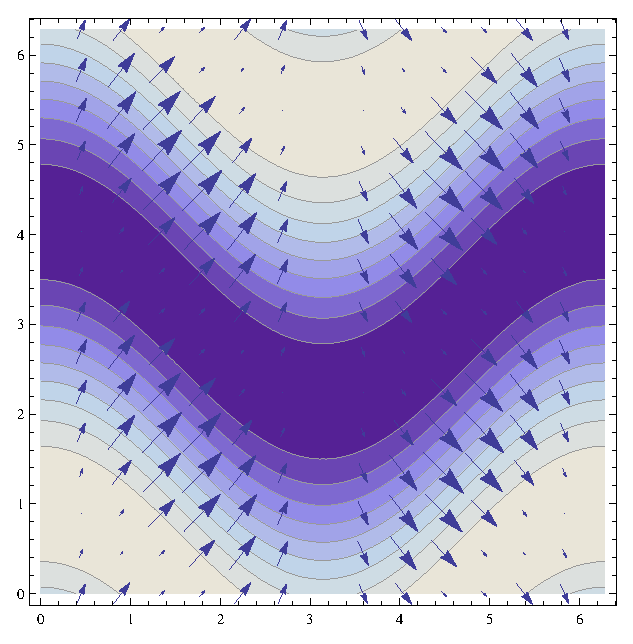
\includegraphics[scale=0.5]{figure-TM-field-components}
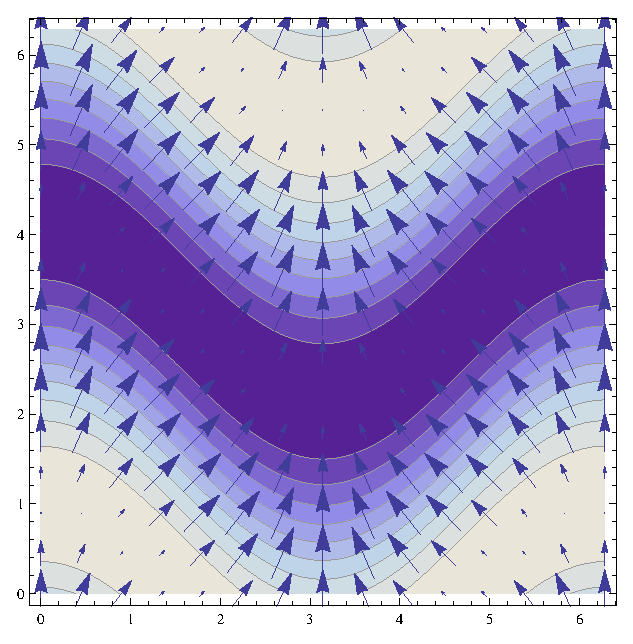
\includegraphics[scale=0.5]{figure-TE-field-components}
\end{center}
\caption{The surface normal components of electric field for (a) TM and (b) TE polarized light.}
\end{figure}
We can now examine the functional form of the allowed normal electric field in the propagation direction for a SPP. The components, $E_{TE}$ and $E_{TM}$, of the electric field normal to the surface, lying along the direction of propagation (the $\mathbf{\hat{x}}$ direction) and integrated over $\mathbf{y}$ for both polarization cases are,
\begin{align}
E_{TM}& = -\frac{4\pi \sin^2{(x)}}{\cos{(2x)-3}}\\
E_{TE} &= -\frac{4\pi \sin{(x)}}{\cos{(2x)-3}}
\end{align}
A plot of $E_{TM}$ and $E_{TE}$ are shown in figure \ref{fig:e-te-and-e-tm}. 
\begin{figure}
\begin{center}
% Created by tikzDevice version 0.6.2-92-0ad2792 on 2012-09-27 16:51:00
% !TEX encoding = UTF-8 Unicode
\begin{tikzpicture}[x=1pt,y=1pt]
\definecolor[named]{fillColor}{rgb}{1.00,1.00,1.00}
\path[use as bounding box,fill=fillColor,fill opacity=0.00] (0,0) rectangle (216.81,216.81);
\begin{scope}
\path[clip] (  0.00,  0.00) rectangle (216.81,216.81);
\definecolor[named]{drawColor}{rgb}{0.00,0.00,0.00}

\path[draw=drawColor,line width= 0.4pt,line join=round,line cap=round] ( 31.20, 49.20) --
	(185.61, 49.20) --
	(185.61,203.61) --
	( 31.20,203.61) --
	( 31.20, 49.20);
\end{scope}
\begin{scope}
\path[clip] (  0.00,  0.00) rectangle (216.81,216.81);
\definecolor[named]{drawColor}{rgb}{0.00,0.00,0.00}

\node[text=drawColor,anchor=base,inner sep=0pt, outer sep=0pt, scale=  1.00] at (108.41,  3.60) {$x$};
\end{scope}
\begin{scope}
\path[clip] (  0.00,  0.00) rectangle (216.81,216.81);
\definecolor[named]{drawColor}{rgb}{0.00,0.00,0.00}

\node[text=drawColor,rotate= 90.00,anchor=base,inner sep=0pt, outer sep=0pt, scale=  1.00] at ( 16.80,126.41) {$E$};
\end{scope}
\begin{scope}
\path[clip] ( 31.20, 49.20) rectangle (185.61,203.61);
\definecolor[named]{drawColor}{rgb}{0.00,0.00,0.00}

\path[draw=drawColor,line width= 0.8pt,line join=round,line cap=round] ( 31.20,126.41) --
	( 32.76,126.97) --
	( 34.32,128.62) --
	( 35.88,131.26) --
	( 37.44,134.73) --
	( 39.00,138.86) --
	( 40.56,143.44) --
	( 42.12,148.29) --
	( 43.68,153.24) --
	( 45.24,158.15) --
	( 46.80,162.92) --
	( 48.36,167.45) --
	( 49.92,171.69) --
	( 51.48,175.60) --
	( 53.04,179.18) --
	( 54.60,182.40) --
	( 56.16,185.26) --
	( 57.71,187.78) --
	( 59.27,189.96) --
	( 60.83,191.82) --
	( 62.39,193.35) --
	( 63.95,194.59) --
	( 65.51,195.52) --
	( 67.07,196.16) --
	( 68.63,196.51) --
	( 70.19,196.58) --
	( 71.75,196.37) --
	( 73.31,195.87) --
	( 74.87,195.09) --
	( 76.43,194.01) --
	( 77.99,192.63) --
	( 79.55,190.93) --
	( 81.11,188.91) --
	( 82.67,186.56) --
	( 84.23,183.87) --
	( 85.79,180.83) --
	( 87.35,177.43) --
	( 88.91,173.69) --
	( 90.47,169.61) --
	( 92.03,165.21) --
	( 93.59,160.56) --
	( 95.15,155.71) --
	( 96.71,150.76) --
	( 98.27,145.84) --
	( 99.83,141.11) --
	(101.39,136.73) --
	(102.95,132.90) --
	(104.51,129.82) --
	(106.07,127.66) --
	(107.63,126.55) --
	(109.18,126.55) --
	(110.74,127.66) --
	(112.30,129.82) --
	(113.86,132.90) --
	(115.42,136.73) --
	(116.98,141.11) --
	(118.54,145.84) --
	(120.10,150.76) --
	(121.66,155.71) --
	(123.22,160.56) --
	(124.78,165.21) --
	(126.34,169.61) --
	(127.90,173.69) --
	(129.46,177.43) --
	(131.02,180.83) --
	(132.58,183.87) --
	(134.14,186.56) --
	(135.70,188.91) --
	(137.26,190.93) --
	(138.82,192.63) --
	(140.38,194.01) --
	(141.94,195.09) --
	(143.50,195.87) --
	(145.06,196.37) --
	(146.62,196.58) --
	(148.18,196.51) --
	(149.74,196.16) --
	(151.30,195.52) --
	(152.86,194.59) --
	(154.42,193.35) --
	(155.98,191.82) --
	(157.54,189.96) --
	(159.10,187.78) --
	(160.65,185.26) --
	(162.21,182.40) --
	(163.77,179.18) --
	(165.33,175.60) --
	(166.89,171.69) --
	(168.45,167.45) --
	(170.01,162.92) --
	(171.57,158.15) --
	(173.13,153.24) --
	(174.69,148.29) --
	(176.25,143.44) --
	(177.81,138.86) --
	(179.37,134.73) --
	(180.93,131.26) --
	(182.49,128.62) --
	(184.05,126.97) --
	(185.61,126.41);
\definecolor[named]{drawColor}{rgb}{1.00,0.00,0.00}

\path[draw=drawColor,line width= 0.8pt,line join=round,line cap=round] ( 31.20,126.41) --
	( 32.76,135.27) --
	( 34.32,143.89) --
	( 35.88,152.05) --
	( 37.44,159.57) --
	( 39.00,166.32) --
	( 40.56,172.24) --
	( 42.12,177.33) --
	( 43.68,181.61) --
	( 45.24,185.13) --
	( 46.80,187.99) --
	( 48.36,190.25) --
	( 49.92,192.02) --
	( 51.48,193.38) --
	( 53.04,194.40) --
	( 54.60,195.14) --
	( 56.16,195.67) --
	( 57.71,196.04) --
	( 59.27,196.28) --
	( 60.83,196.43) --
	( 62.39,196.52) --
	( 63.95,196.56) --
	( 65.51,196.58) --
	( 67.07,196.59) --
	( 68.63,196.59) --
	( 70.19,196.59) --
	( 71.75,196.59) --
	( 73.31,196.59) --
	( 74.87,196.58) --
	( 76.43,196.54) --
	( 77.99,196.48) --
	( 79.55,196.36) --
	( 81.11,196.17) --
	( 82.67,195.87) --
	( 84.23,195.43) --
	( 85.79,194.80) --
	( 87.35,193.93) --
	( 88.91,192.75) --
	( 90.47,191.20) --
	( 92.03,189.19) --
	( 93.59,186.64) --
	( 95.15,183.46) --
	( 96.71,179.57) --
	( 98.27,174.89) --
	( 99.83,169.39) --
	(101.39,163.04) --
	(102.95,155.90) --
	(104.51,148.04) --
	(106.07,139.63) --
	(107.63,130.85) --
	(109.18,121.96) --
	(110.74,113.18) --
	(112.30,104.77) --
	(113.86, 96.91) --
	(115.42, 89.77) --
	(116.98, 83.42) --
	(118.54, 77.92) --
	(120.10, 73.24) --
	(121.66, 69.35) --
	(123.22, 66.17) --
	(124.78, 63.62) --
	(126.34, 61.61) --
	(127.90, 60.06) --
	(129.46, 58.88) --
	(131.02, 58.01) --
	(132.58, 57.38) --
	(134.14, 56.94) --
	(135.70, 56.64) --
	(137.26, 56.45) --
	(138.82, 56.33) --
	(140.38, 56.27) --
	(141.94, 56.23) --
	(143.50, 56.22) --
	(145.06, 56.22) --
	(146.62, 56.22) --
	(148.18, 56.22) --
	(149.74, 56.22) --
	(151.30, 56.23) --
	(152.86, 56.25) --
	(154.42, 56.29) --
	(155.98, 56.38) --
	(157.54, 56.53) --
	(159.10, 56.77) --
	(160.65, 57.14) --
	(162.21, 57.67) --
	(163.77, 58.41) --
	(165.33, 59.43) --
	(166.89, 60.79) --
	(168.45, 62.56) --
	(170.01, 64.82) --
	(171.57, 67.68) --
	(173.13, 71.20) --
	(174.69, 75.48) --
	(176.25, 80.57) --
	(177.81, 86.49) --
	(179.37, 93.24) --
	(180.93,100.76) --
	(182.49,108.92) --
	(184.05,117.54) --
	(185.61,126.40);
\definecolor[named]{drawColor}{rgb}{0.00,0.00,0.00}

\path[draw=drawColor,line width= 0.4pt,line join=round,line cap=round] ( 31.20,126.41) --
	( 32.76,126.41) --
	( 34.32,126.41) --
	( 35.88,126.41) --
	( 37.44,126.41) --
	( 39.00,126.41) --
	( 40.56,126.41) --
	( 42.12,126.41) --
	( 43.68,126.41) --
	( 45.24,126.41) --
	( 46.80,126.41) --
	( 48.36,126.41) --
	( 49.92,126.41) --
	( 51.48,126.41) --
	( 53.04,126.41) --
	( 54.60,126.41) --
	( 56.16,126.41) --
	( 57.71,126.41) --
	( 59.27,126.41) --
	( 60.83,126.41) --
	( 62.39,126.41) --
	( 63.95,126.41) --
	( 65.51,126.41) --
	( 67.07,126.41) --
	( 68.63,126.41) --
	( 70.19,126.41) --
	( 71.75,126.41) --
	( 73.31,126.41) --
	( 74.87,126.41) --
	( 76.43,126.41) --
	( 77.99,126.41) --
	( 79.55,126.41) --
	( 81.11,126.41) --
	( 82.67,126.41) --
	( 84.23,126.41) --
	( 85.79,126.41) --
	( 87.35,126.41) --
	( 88.91,126.41) --
	( 90.47,126.41) --
	( 92.03,126.41) --
	( 93.59,126.41) --
	( 95.15,126.41) --
	( 96.71,126.41) --
	( 98.27,126.41) --
	( 99.83,126.41) --
	(101.39,126.41) --
	(102.95,126.41) --
	(104.51,126.41) --
	(106.07,126.41) --
	(107.63,126.41) --
	(109.18,126.41) --
	(110.74,126.41) --
	(112.30,126.41) --
	(113.86,126.41) --
	(115.42,126.41) --
	(116.98,126.41) --
	(118.54,126.41) --
	(120.10,126.41) --
	(121.66,126.41) --
	(123.22,126.41) --
	(124.78,126.41) --
	(126.34,126.41) --
	(127.90,126.41) --
	(129.46,126.41) --
	(131.02,126.41) --
	(132.58,126.41) --
	(134.14,126.41) --
	(135.70,126.41) --
	(137.26,126.41) --
	(138.82,126.41) --
	(140.38,126.41) --
	(141.94,126.41) --
	(143.50,126.41) --
	(145.06,126.41) --
	(146.62,126.41) --
	(148.18,126.41) --
	(149.74,126.41) --
	(151.30,126.41) --
	(152.86,126.41) --
	(154.42,126.41) --
	(155.98,126.41) --
	(157.54,126.41) --
	(159.10,126.41) --
	(160.65,126.41) --
	(162.21,126.41) --
	(163.77,126.41) --
	(165.33,126.41) --
	(166.89,126.41) --
	(168.45,126.41) --
	(170.01,126.41) --
	(171.57,126.41) --
	(173.13,126.41) --
	(174.69,126.41) --
	(176.25,126.41) --
	(177.81,126.41) --
	(179.37,126.41) --
	(180.93,126.41) --
	(182.49,126.41) --
	(184.05,126.41) --
	(185.61,126.41);
\definecolor[named]{drawColor}{rgb}{1.00,0.00,0.00}

\node[text=drawColor,anchor=base west,inner sep=0pt, outer sep=0pt, scale=  1.00] at (120.76, 90.60) {$E_{TE}$};
\definecolor[named]{drawColor}{rgb}{0.00,0.00,0.00}

\node[text=drawColor,anchor=base east,inner sep=0pt, outer sep=0pt, scale=  1.00] at (160.85,168.79) {$E_{TM}$};
\end{scope}
\begin{scope}
\path[clip] (  0.00,  0.00) rectangle (216.81,216.81);
\definecolor[named]{drawColor}{rgb}{0.00,0.00,0.00}

\path[draw=drawColor,line width= 0.4pt,line join=round,line cap=round] ( 31.20, 49.20) -- (185.61, 49.20);

\path[draw=drawColor,line width= 0.4pt,line join=round,line cap=round] ( 31.20, 49.20) -- ( 31.20, 43.20);

\path[draw=drawColor,line width= 0.4pt,line join=round,line cap=round] (108.41, 49.20) -- (108.41, 43.20);

\path[draw=drawColor,line width= 0.4pt,line join=round,line cap=round] (185.61, 49.20) -- (185.61, 43.20);

\node[text=drawColor,anchor=base,inner sep=0pt, outer sep=0pt, scale=  1.00] at ( 31.20, 27.60) {0};

\node[text=drawColor,anchor=base,inner sep=0pt, outer sep=0pt, scale=  1.00] at (108.41, 27.60) {$\pi$};

\node[text=drawColor,anchor=base,inner sep=0pt, outer sep=0pt, scale=  1.00] at (185.61, 27.60) {$2\pi$};
\end{scope}
\end{tikzpicture}

\caption{The magnitude of the surface normal electric field in the x-directio for TM and TE polarisations.\label{fig:e-te-and-e-tm}}
\end{center}
\end{figure}
Both $E_{TE}$ and $E_{TM}$ are non-zero, so we may conclude that either polarization may induce surface charge and possibly excite SPPs. By expanding both these expressions as a Fourier sum in x, it is possible to find which in-plane wavevectors of incident light are required to match these field profiles. Doing so yields,
\begin{align}
E_{TM}=&\sum\limits_{n=1,3,5,...}^\infty a_n\cos{(nx)}\\
E_{TE}=&\;a_0+\displaystyle\sum\limits_{n=2,4,6,...}^\infty b_n\sin{(nx)}\label{eq:odd-even-fouriers}
\end{align}
Where $a_n$ and $b_n$ are the Fourier series coefficents. For incident light to match $E_{TE}$ requires a series of only odd-ordered terms, while $E_{TM}$ requires a series of only even-ordered terms. Diffracted fields at the surface will contain both odd distributive even wavevector components. Equations 2 and 3 predict that TE polarized light will provide a suitable electric field distribution to enable the excitation of SPPs via only odd-ordered diffracted orders, while TM polarized light will excite SPPs only via even-ordered diffracted orders.  This concept will be discussed again with reference to the experimental and modelled results in section 4.
We can visualise these coupling conditions in a simplistic diagrammatic way, shown in in figure \ref{fig:coupling-cartoon}.
\begin{figure}
\begin{center}
% Created by tikzDevice version 0.6.2-92-0ad2792 on 2012-12-18 10:42:07
% !TEX encoding = UTF-8 Unicode
\begin{tikzpicture}[x=1pt,y=1pt]
\definecolor[named]{fillColor}{rgb}{1.00,1.00,1.00}
\path[use as bounding box,fill=fillColor,fill opacity=0.00] (0,0) rectangle (433.62,361.35);
\begin{scope}
\path[clip] (  0.00,180.67) rectangle (216.81,361.35);
\definecolor[named]{drawColor}{rgb}{0.00,0.00,0.00}

\node[text=drawColor,anchor=base,inner sep=0pt, outer sep=0pt, scale=  0.83] at (108.41,152.79) {x};

\path[draw=drawColor,line width= 0.4pt,line join=round,line cap=round] ( 26.47,222.74) -- ( 31.30,227.56);

\path[draw=drawColor,line width= 0.4pt,line join=round,line cap=round] ( 26.47,215.92) -- ( 42.11,231.56);

\path[draw=drawColor,line width= 0.4pt,line join=round,line cap=round] ( 26.47,209.11) -- ( 52.92,235.56);

\path[draw=drawColor,line width= 0.4pt,line join=round,line cap=round] ( 26.47,202.30) -- ( 63.73,239.55);

\path[draw=drawColor,line width= 0.4pt,line join=round,line cap=round] ( 26.47,195.48) -- ( 74.54,243.55);

\path[draw=drawColor,line width= 0.4pt,line join=round,line cap=round] ( 37.29,199.48) -- ( 85.36,247.55);

\path[draw=drawColor,line width= 0.4pt,line join=round,line cap=round] ( 48.10,203.48) -- ( 96.17,251.55);

\path[draw=drawColor,line width= 0.4pt,line join=round,line cap=round] ( 58.91,207.48) -- (106.98,255.54);

\path[draw=drawColor,line width= 0.4pt,line join=round,line cap=round] ( 69.72,211.47) -- (112.72,254.48);

\path[draw=drawColor,line width= 0.4pt,line join=round,line cap=round] ( 80.53,215.47) -- (117.70,252.64);

\path[draw=drawColor,line width= 0.4pt,line join=round,line cap=round] ( 91.34,219.47) -- (122.67,250.80);

\path[draw=drawColor,line width= 0.4pt,line join=round,line cap=round] (102.15,223.47) -- (127.65,248.96);

\path[draw=drawColor,line width= 0.4pt,line join=round,line cap=round] (110.50,225.00) -- (132.62,247.12);

\path[draw=drawColor,line width= 0.4pt,line join=round,line cap=round] (115.48,223.16) -- (137.59,245.28);

\path[draw=drawColor,line width= 0.4pt,line join=round,line cap=round] (120.45,221.32) -- (142.57,243.44);

\path[draw=drawColor,line width= 0.4pt,line join=round,line cap=round] (125.43,219.48) -- (147.54,241.60);

\path[draw=drawColor,line width= 0.4pt,line join=round,line cap=round] (130.40,217.64) -- (152.52,239.76);

\path[draw=drawColor,line width= 0.4pt,line join=round,line cap=round] (135.37,215.80) -- (157.49,237.92);

\path[draw=drawColor,line width= 0.4pt,line join=round,line cap=round] (140.35,213.97) -- (162.47,236.08);

\path[draw=drawColor,line width= 0.4pt,line join=round,line cap=round] (145.32,212.13) -- (167.44,234.24);

\path[draw=drawColor,line width= 0.4pt,line join=round,line cap=round] (150.30,210.29) -- (172.41,232.40);

\path[draw=drawColor,line width= 0.4pt,line join=round,line cap=round] (155.27,208.45) -- (177.39,230.56);

\path[draw=drawColor,line width= 0.4pt,line join=round,line cap=round] (160.25,206.61) -- (182.36,228.73);

\path[draw=drawColor,line width= 0.4pt,line join=round,line cap=round] (165.22,204.77) -- (187.34,226.89);

\path[draw=drawColor,line width= 0.4pt,line join=round,line cap=round] (170.20,202.93) -- (190.34,223.07);

\path[draw=drawColor,line width= 0.4pt,line join=round,line cap=round] (175.17,201.09) -- (190.34,216.26);

\path[draw=drawColor,line width= 0.4pt,line join=round,line cap=round] (180.14,199.25) -- (190.34,209.44);

\path[draw=drawColor,line width= 0.4pt,line join=round,line cap=round] (185.12,197.41) -- (190.34,202.63);

\path[draw=drawColor,line width= 0.4pt,line join=round,line cap=round] (190.09,195.57) -- (190.34,195.81);

\path[draw=drawColor,line width= 0.4pt,line join=round,line cap=round] ( 26.47,195.48) --
	( 26.47,225.78) --
	(108.41,256.07) --
	(190.34,225.78) --
	(190.34,195.48) --
	(108.41,225.78) --
	( 26.47,195.48);

\path[draw=drawColor,line width= 0.4pt,line join=round,line cap=round] ( 26.47,284.06) -- ( 30.14,287.72);

\path[draw=drawColor,line width= 0.4pt,line join=round,line cap=round] ( 26.47,277.25) -- ( 40.95,291.72);

\path[draw=drawColor,line width= 0.4pt,line join=round,line cap=round] ( 26.47,270.43) -- ( 51.76,295.72);

\path[draw=drawColor,line width= 0.4pt,line join=round,line cap=round] ( 26.47,263.62) -- ( 62.57,299.71);

\path[draw=drawColor,line width= 0.4pt,line join=round,line cap=round] ( 26.47,256.81) -- ( 73.38,303.71);

\path[draw=drawColor,line width= 0.4pt,line join=round,line cap=round] ( 36.12,259.64) -- ( 84.19,307.71);

\path[draw=drawColor,line width= 0.4pt,line join=round,line cap=round] ( 46.93,263.64) -- ( 95.00,311.71);

\path[draw=drawColor,line width= 0.4pt,line join=round,line cap=round] ( 57.75,267.64) -- (105.82,315.71);

\path[draw=drawColor,line width= 0.4pt,line join=round,line cap=round] ( 68.56,271.63) -- (112.19,315.26);

\path[draw=drawColor,line width= 0.4pt,line join=round,line cap=round] ( 79.37,275.63) -- (117.16,313.42);

\path[draw=drawColor,line width= 0.4pt,line join=round,line cap=round] ( 90.18,279.63) -- (122.14,311.59);

\path[draw=drawColor,line width= 0.4pt,line join=round,line cap=round] (100.99,283.63) -- (127.11,309.75);

\path[draw=drawColor,line width= 0.4pt,line join=round,line cap=round] (109.97,285.79) -- (132.09,307.91);

\path[draw=drawColor,line width= 0.4pt,line join=round,line cap=round] (114.94,283.95) -- (137.06,306.07);

\path[draw=drawColor,line width= 0.4pt,line join=round,line cap=round] (119.92,282.11) -- (142.03,304.23);

\path[draw=drawColor,line width= 0.4pt,line join=round,line cap=round] (124.89,280.27) -- (147.01,302.39);

\path[draw=drawColor,line width= 0.4pt,line join=round,line cap=round] (129.87,278.43) -- (151.98,300.55);

\path[draw=drawColor,line width= 0.4pt,line join=round,line cap=round] (134.84,276.59) -- (156.96,298.71);

\path[draw=drawColor,line width= 0.4pt,line join=round,line cap=round] (139.81,274.75) -- (161.93,296.87);

\path[draw=drawColor,line width= 0.4pt,line join=round,line cap=round] (144.79,272.91) -- (166.91,295.03);

\path[draw=drawColor,line width= 0.4pt,line join=round,line cap=round] (149.76,271.07) -- (171.88,293.19);

\path[draw=drawColor,line width= 0.4pt,line join=round,line cap=round] (154.74,269.24) -- (176.85,291.35);

\path[draw=drawColor,line width= 0.4pt,line join=round,line cap=round] (159.71,267.40) -- (181.83,289.51);

\path[draw=drawColor,line width= 0.4pt,line join=round,line cap=round] (164.69,265.56) -- (186.80,287.67);

\path[draw=drawColor,line width= 0.4pt,line join=round,line cap=round] (169.66,263.72) -- (190.34,284.39);

\path[draw=drawColor,line width= 0.4pt,line join=round,line cap=round] (174.63,261.88) -- (190.34,277.58);

\path[draw=drawColor,line width= 0.4pt,line join=round,line cap=round] (179.61,260.04) -- (190.34,270.77);

\path[draw=drawColor,line width= 0.4pt,line join=round,line cap=round] (184.58,258.20) -- (190.34,263.95);

\path[draw=drawColor,line width= 0.4pt,line join=round,line cap=round] (189.56,256.36) -- (190.34,257.14);

\path[draw=drawColor,line width= 0.4pt,line join=round,line cap=round] ( 26.47,256.07) --
	( 26.47,286.37) --
	(108.41,316.66) --
	(190.34,286.37) --
	(190.34,256.07) --
	(108.41,286.37) --
	( 26.47,256.07);
\definecolor[named]{fillColor}{rgb}{1.00,1.00,1.00}

\path[fill=fillColor,fill opacity=0.75] ( 26.47,225.78) circle (  3.73);

\path[fill=fillColor,fill opacity=0.75] ( 46.96,233.45) circle (  3.73);

\path[fill=fillColor,fill opacity=0.75] ( 67.44,240.92) circle (  3.73);

\path[fill=fillColor,fill opacity=0.75] ( 87.92,248.40) circle (  3.73);

\path[fill=fillColor,fill opacity=0.75] (108.41,256.07) circle (  3.73);

\path[fill=fillColor,fill opacity=0.75] (128.89,248.40) circle (  3.73);

\path[fill=fillColor,fill opacity=0.75] (149.37,240.92) circle (  3.73);

\path[fill=fillColor,fill opacity=0.75] (169.85,233.45) circle (  3.73);

\path[fill=fillColor,fill opacity=0.75] (190.34,225.78) circle (  3.73);

\path[fill=fillColor,fill opacity=0.75] ( 26.47,256.07) circle (  3.73);

\path[fill=fillColor,fill opacity=0.75] ( 46.96,263.75) circle (  3.73);

\path[fill=fillColor,fill opacity=0.75] ( 67.44,271.22) circle (  3.73);

\path[fill=fillColor,fill opacity=0.75] ( 87.92,278.69) circle (  3.73);

\path[fill=fillColor,fill opacity=0.75] (108.41,286.37) circle (  3.73);

\path[fill=fillColor,fill opacity=0.75] (128.89,278.69) circle (  3.73);

\path[fill=fillColor,fill opacity=0.75] (149.37,271.22) circle (  3.73);

\path[fill=fillColor,fill opacity=0.75] (169.85,263.75) circle (  3.73);

\path[fill=fillColor,fill opacity=0.75] (190.34,256.07) circle (  3.73);

\path[fill=fillColor,fill opacity=0.75] ( 26.47,286.37) circle (  3.73);

\path[fill=fillColor,fill opacity=0.75] ( 46.96,294.04) circle (  3.73);

\path[fill=fillColor,fill opacity=0.75] ( 67.44,301.52) circle (  3.73);

\path[fill=fillColor,fill opacity=0.75] ( 87.92,308.99) circle (  3.73);

\path[fill=fillColor,fill opacity=0.75] (108.41,316.66) circle (  3.73);

\path[fill=fillColor,fill opacity=0.75] (128.89,308.99) circle (  3.73);

\path[fill=fillColor,fill opacity=0.75] (149.37,301.52) circle (  3.73);

\path[fill=fillColor,fill opacity=0.75] (169.85,294.04) circle (  3.73);

\path[fill=fillColor,fill opacity=0.75] (190.34,286.37) circle (  3.73);

\path[fill=fillColor,fill opacity=0.75] ( 26.47,195.48) circle (  3.73);

\path[fill=fillColor,fill opacity=0.75] ( 46.96,203.16) circle (  3.73);

\path[fill=fillColor,fill opacity=0.75] ( 67.44,210.63) circle (  3.73);

\path[fill=fillColor,fill opacity=0.75] ( 87.92,218.10) circle (  3.73);

\path[fill=fillColor,fill opacity=0.75] (108.41,225.78) circle (  3.73);

\path[fill=fillColor,fill opacity=0.75] (128.89,218.10) circle (  3.73);

\path[fill=fillColor,fill opacity=0.75] (149.37,210.63) circle (  3.73);

\path[fill=fillColor,fill opacity=0.75] (169.85,203.16) circle (  3.73);

\path[fill=fillColor,fill opacity=0.75] (190.34,195.48) circle (  3.73);

\node[text=drawColor,anchor=base,inner sep=0pt, outer sep=0pt, scale=  1.66] at ( 26.47,220.25) {$+$};

\node[text=drawColor,anchor=base,inner sep=0pt, outer sep=0pt, scale=  1.66] at ( 46.96,227.92) {$+$};

\node[text=drawColor,anchor=base,inner sep=0pt, outer sep=0pt, scale=  1.66] at ( 67.44,235.39) {$+$};

\node[text=drawColor,anchor=base,inner sep=0pt, outer sep=0pt, scale=  1.66] at ( 87.92,242.87) {$+$};

\node[text=drawColor,anchor=base,inner sep=0pt, outer sep=0pt, scale=  1.66] at (108.41,250.54) {$+$};

\node[text=drawColor,anchor=base,inner sep=0pt, outer sep=0pt, scale=  1.66] at (128.89,242.87) {$+$};

\node[text=drawColor,anchor=base,inner sep=0pt, outer sep=0pt, scale=  1.66] at (149.37,235.39) {$+$};

\node[text=drawColor,anchor=base,inner sep=0pt, outer sep=0pt, scale=  1.66] at (169.85,227.92) {$+$};

\node[text=drawColor,anchor=base,inner sep=0pt, outer sep=0pt, scale=  1.66] at (190.34,220.25) {$+$};

\node[text=drawColor,anchor=base,inner sep=0pt, outer sep=0pt, scale=  1.66] at ( 26.47,250.31) {$-$};

\node[text=drawColor,anchor=base,inner sep=0pt, outer sep=0pt, scale=  1.66] at ( 46.96,257.98) {$-$};

\node[text=drawColor,anchor=base,inner sep=0pt, outer sep=0pt, scale=  1.66] at ( 67.44,265.46) {$-$};

\node[text=drawColor,anchor=base,inner sep=0pt, outer sep=0pt, scale=  1.66] at ( 87.92,272.93) {$-$};

\node[text=drawColor,anchor=base,inner sep=0pt, outer sep=0pt, scale=  1.66] at (108.41,280.61) {$-$};

\node[text=drawColor,anchor=base,inner sep=0pt, outer sep=0pt, scale=  1.66] at (128.89,272.93) {$-$};

\node[text=drawColor,anchor=base,inner sep=0pt, outer sep=0pt, scale=  1.66] at (149.37,265.46) {$-$};

\node[text=drawColor,anchor=base,inner sep=0pt, outer sep=0pt, scale=  1.66] at (169.85,257.98) {$-$};

\node[text=drawColor,anchor=base,inner sep=0pt, outer sep=0pt, scale=  1.66] at (190.34,250.31) {$-$};

\node[text=drawColor,anchor=base,inner sep=0pt, outer sep=0pt, scale=  1.66] at ( 26.47,280.84) {$+$};

\node[text=drawColor,anchor=base,inner sep=0pt, outer sep=0pt, scale=  1.66] at ( 46.96,288.51) {$+$};

\node[text=drawColor,anchor=base,inner sep=0pt, outer sep=0pt, scale=  1.66] at ( 67.44,295.98) {$+$};

\node[text=drawColor,anchor=base,inner sep=0pt, outer sep=0pt, scale=  1.66] at ( 87.92,303.46) {$+$};

\node[text=drawColor,anchor=base,inner sep=0pt, outer sep=0pt, scale=  1.66] at (108.41,311.13) {$+$};

\node[text=drawColor,anchor=base,inner sep=0pt, outer sep=0pt, scale=  1.66] at (128.89,303.46) {$+$};

\node[text=drawColor,anchor=base,inner sep=0pt, outer sep=0pt, scale=  1.66] at (149.37,295.98) {$+$};

\node[text=drawColor,anchor=base,inner sep=0pt, outer sep=0pt, scale=  1.66] at (169.85,288.51) {$+$};

\node[text=drawColor,anchor=base,inner sep=0pt, outer sep=0pt, scale=  1.66] at (190.34,280.84) {$+$};

\node[text=drawColor,anchor=base,inner sep=0pt, outer sep=0pt, scale=  1.66] at ( 26.47,189.72) {$-$};

\node[text=drawColor,anchor=base,inner sep=0pt, outer sep=0pt, scale=  1.66] at ( 46.96,197.39) {$-$};

\node[text=drawColor,anchor=base,inner sep=0pt, outer sep=0pt, scale=  1.66] at ( 67.44,204.87) {$-$};

\node[text=drawColor,anchor=base,inner sep=0pt, outer sep=0pt, scale=  1.66] at ( 87.92,212.34) {$-$};

\node[text=drawColor,anchor=base,inner sep=0pt, outer sep=0pt, scale=  1.66] at (108.41,220.01) {$-$};

\node[text=drawColor,anchor=base,inner sep=0pt, outer sep=0pt, scale=  1.66] at (128.89,212.34) {$-$};

\node[text=drawColor,anchor=base,inner sep=0pt, outer sep=0pt, scale=  1.66] at (149.37,204.87) {$-$};

\node[text=drawColor,anchor=base,inner sep=0pt, outer sep=0pt, scale=  1.66] at (169.85,197.39) {$-$};

\node[text=drawColor,anchor=base,inner sep=0pt, outer sep=0pt, scale=  1.66] at (190.34,189.72) {$-$};

\path[draw=drawColor,line width= 1.2pt,line join=round,line cap=round] (163.03,324.74) -- (163.03,357.06);

\path[draw=drawColor,line width= 1.2pt,line join=round,line cap=round] (168.45,347.67) --
	(163.03,357.06) --
	(157.61,347.67);

\node[text=drawColor,anchor=base west,inner sep=0pt, outer sep=0pt, scale=  0.83] at (168.01,334.95) {$\mathbf{E}$};

\path[draw=drawColor,line width= 1.2pt,line join=round,line cap=round] ( 67.44,240.92) -- ( 57.88,263.75);

\path[draw=drawColor,line width= 1.2pt,line join=round,line cap=round] ( 66.51,257.18) --
	( 57.88,263.75) --
	( 56.51,252.99);

\path[draw=drawColor,line width= 1.2pt,line join=round,line cap=round] (149.37,240.92) -- (158.93,263.75);

\path[draw=drawColor,line width= 1.2pt,line join=round,line cap=round] (160.30,252.99) --
	(158.93,263.75) --
	(150.30,257.18);
\definecolor[named]{drawColor}{rgb}{1.00,0.00,0.00}

\path[draw=drawColor,line width= 1.2pt,line join=round,line cap=round] ( 67.44,240.92) -- ( 46.96,240.92);

\path[draw=drawColor,line width= 1.2pt,line join=round,line cap=round] ( 56.35,246.35) --
	( 46.96,240.92) --
	( 56.35,235.50);

\path[draw=drawColor,line width= 1.2pt,line join=round,line cap=round] (149.37,240.92) -- (169.85,240.92);

\path[draw=drawColor,line width= 1.2pt,line join=round,line cap=round] (160.46,235.50) --
	(169.85,240.92) --
	(160.46,246.35);
\definecolor[named]{fillColor}{rgb}{1.00,0.00,0.00}

\path[fill=fillColor] ( 26.47,240.92) circle (  1.87);

\path[fill=fillColor] (108.41,271.22) circle (  1.87);

\path[fill=fillColor] (190.34,240.92) circle (  1.87);
\definecolor[named]{drawColor}{rgb}{0.00,0.00,0.00}

\node[text=drawColor,anchor=base,inner sep=0pt, outer sep=0pt, scale=  1.00] at (108.41,337.99) {\bfseries TE};
\end{scope}
\begin{scope}
\path[clip] (216.81,180.67) rectangle (433.62,361.35);
\definecolor[named]{drawColor}{rgb}{0.00,0.00,0.00}

\path[draw=drawColor,line width= 0.4pt,line join=round,line cap=round] (243.28,222.74) -- (248.11,227.56);

\path[draw=drawColor,line width= 0.4pt,line join=round,line cap=round] (243.28,215.92) -- (258.92,231.56);

\path[draw=drawColor,line width= 0.4pt,line join=round,line cap=round] (243.28,209.11) -- (269.73,235.56);

\path[draw=drawColor,line width= 0.4pt,line join=round,line cap=round] (243.28,202.30) -- (280.54,239.55);

\path[draw=drawColor,line width= 0.4pt,line join=round,line cap=round] (243.28,195.48) -- (291.35,243.55);

\path[draw=drawColor,line width= 0.4pt,line join=round,line cap=round] (254.10,199.48) -- (302.17,247.55);

\path[draw=drawColor,line width= 0.4pt,line join=round,line cap=round] (264.91,203.48) -- (312.98,251.55);

\path[draw=drawColor,line width= 0.4pt,line join=round,line cap=round] (275.72,207.48) -- (323.79,255.54);

\path[draw=drawColor,line width= 0.4pt,line join=round,line cap=round] (286.53,211.47) -- (329.53,254.48);

\path[draw=drawColor,line width= 0.4pt,line join=round,line cap=round] (297.34,215.47) -- (334.51,252.64);

\path[draw=drawColor,line width= 0.4pt,line join=round,line cap=round] (308.15,219.47) -- (339.48,250.80);

\path[draw=drawColor,line width= 0.4pt,line join=round,line cap=round] (318.96,223.47) -- (344.46,248.96);

\path[draw=drawColor,line width= 0.4pt,line join=round,line cap=round] (327.31,225.00) -- (349.43,247.12);

\path[draw=drawColor,line width= 0.4pt,line join=round,line cap=round] (332.29,223.16) -- (354.40,245.28);

\path[draw=drawColor,line width= 0.4pt,line join=round,line cap=round] (337.26,221.32) -- (359.38,243.44);

\path[draw=drawColor,line width= 0.4pt,line join=round,line cap=round] (342.24,219.48) -- (364.35,241.60);

\path[draw=drawColor,line width= 0.4pt,line join=round,line cap=round] (347.21,217.64) -- (369.33,239.76);

\path[draw=drawColor,line width= 0.4pt,line join=round,line cap=round] (352.18,215.80) -- (374.30,237.92);

\path[draw=drawColor,line width= 0.4pt,line join=round,line cap=round] (357.16,213.97) -- (379.28,236.08);

\path[draw=drawColor,line width= 0.4pt,line join=round,line cap=round] (362.13,212.13) -- (384.25,234.24);

\path[draw=drawColor,line width= 0.4pt,line join=round,line cap=round] (367.11,210.29) -- (389.22,232.40);

\path[draw=drawColor,line width= 0.4pt,line join=round,line cap=round] (372.08,208.45) -- (394.20,230.56);

\path[draw=drawColor,line width= 0.4pt,line join=round,line cap=round] (377.06,206.61) -- (399.17,228.73);

\path[draw=drawColor,line width= 0.4pt,line join=round,line cap=round] (382.03,204.77) -- (404.15,226.89);

\path[draw=drawColor,line width= 0.4pt,line join=round,line cap=round] (387.01,202.93) -- (407.15,223.07);

\path[draw=drawColor,line width= 0.4pt,line join=round,line cap=round] (391.98,201.09) -- (407.15,216.26);

\path[draw=drawColor,line width= 0.4pt,line join=round,line cap=round] (396.95,199.25) -- (407.15,209.44);

\path[draw=drawColor,line width= 0.4pt,line join=round,line cap=round] (401.93,197.41) -- (407.15,202.63);

\path[draw=drawColor,line width= 0.4pt,line join=round,line cap=round] (406.90,195.57) -- (407.15,195.81);

\path[draw=drawColor,line width= 0.4pt,line join=round,line cap=round] (243.28,195.48) --
	(243.28,225.78) --
	(325.22,256.07) --
	(407.15,225.78) --
	(407.15,195.48) --
	(325.22,225.78) --
	(243.28,195.48);

\path[draw=drawColor,line width= 0.4pt,line join=round,line cap=round] (243.28,284.06) -- (246.95,287.72);

\path[draw=drawColor,line width= 0.4pt,line join=round,line cap=round] (243.28,277.25) -- (257.76,291.72);

\path[draw=drawColor,line width= 0.4pt,line join=round,line cap=round] (243.28,270.43) -- (268.57,295.72);

\path[draw=drawColor,line width= 0.4pt,line join=round,line cap=round] (243.28,263.62) -- (279.38,299.71);

\path[draw=drawColor,line width= 0.4pt,line join=round,line cap=round] (243.28,256.81) -- (290.19,303.71);

\path[draw=drawColor,line width= 0.4pt,line join=round,line cap=round] (252.93,259.64) -- (301.00,307.71);

\path[draw=drawColor,line width= 0.4pt,line join=round,line cap=round] (263.74,263.64) -- (311.81,311.71);

\path[draw=drawColor,line width= 0.4pt,line join=round,line cap=round] (274.56,267.64) -- (322.63,315.71);

\path[draw=drawColor,line width= 0.4pt,line join=round,line cap=round] (285.37,271.63) -- (329.00,315.26);

\path[draw=drawColor,line width= 0.4pt,line join=round,line cap=round] (296.18,275.63) -- (333.97,313.42);

\path[draw=drawColor,line width= 0.4pt,line join=round,line cap=round] (306.99,279.63) -- (338.95,311.59);

\path[draw=drawColor,line width= 0.4pt,line join=round,line cap=round] (317.80,283.63) -- (343.92,309.75);

\path[draw=drawColor,line width= 0.4pt,line join=round,line cap=round] (326.78,285.79) -- (348.90,307.91);

\path[draw=drawColor,line width= 0.4pt,line join=round,line cap=round] (331.75,283.95) -- (353.87,306.07);

\path[draw=drawColor,line width= 0.4pt,line join=round,line cap=round] (336.73,282.11) -- (358.84,304.23);

\path[draw=drawColor,line width= 0.4pt,line join=round,line cap=round] (341.70,280.27) -- (363.82,302.39);

\path[draw=drawColor,line width= 0.4pt,line join=round,line cap=round] (346.68,278.43) -- (368.79,300.55);

\path[draw=drawColor,line width= 0.4pt,line join=round,line cap=round] (351.65,276.59) -- (373.77,298.71);

\path[draw=drawColor,line width= 0.4pt,line join=round,line cap=round] (356.62,274.75) -- (378.74,296.87);

\path[draw=drawColor,line width= 0.4pt,line join=round,line cap=round] (361.60,272.91) -- (383.72,295.03);

\path[draw=drawColor,line width= 0.4pt,line join=round,line cap=round] (366.57,271.07) -- (388.69,293.19);

\path[draw=drawColor,line width= 0.4pt,line join=round,line cap=round] (371.55,269.24) -- (393.66,291.35);

\path[draw=drawColor,line width= 0.4pt,line join=round,line cap=round] (376.52,267.40) -- (398.64,289.51);

\path[draw=drawColor,line width= 0.4pt,line join=round,line cap=round] (381.50,265.56) -- (403.61,287.67);

\path[draw=drawColor,line width= 0.4pt,line join=round,line cap=round] (386.47,263.72) -- (407.15,284.39);

\path[draw=drawColor,line width= 0.4pt,line join=round,line cap=round] (391.44,261.88) -- (407.15,277.58);

\path[draw=drawColor,line width= 0.4pt,line join=round,line cap=round] (396.42,260.04) -- (407.15,270.77);

\path[draw=drawColor,line width= 0.4pt,line join=round,line cap=round] (401.39,258.20) -- (407.15,263.95);

\path[draw=drawColor,line width= 0.4pt,line join=round,line cap=round] (406.37,256.36) -- (407.15,257.14);

\path[draw=drawColor,line width= 0.4pt,line join=round,line cap=round] (243.28,256.07) --
	(243.28,286.37) --
	(325.22,316.66) --
	(407.15,286.37) --
	(407.15,256.07) --
	(325.22,286.37) --
	(243.28,256.07);
\definecolor[named]{fillColor}{rgb}{1.00,1.00,1.00}

\path[fill=fillColor,fill opacity=0.75] (263.77,233.45) circle (  3.73);

\path[fill=fillColor,fill opacity=0.75] (284.25,240.92) circle (  3.73);

\path[fill=fillColor,fill opacity=0.75] (304.73,248.40) circle (  3.73);

\path[fill=fillColor,fill opacity=0.75] (345.70,248.40) circle (  3.73);

\path[fill=fillColor,fill opacity=0.75] (366.18,240.92) circle (  3.73);

\path[fill=fillColor,fill opacity=0.75] (386.66,233.45) circle (  3.73);

\path[fill=fillColor,fill opacity=0.75] (263.77,263.75) circle (  3.73);

\path[fill=fillColor,fill opacity=0.75] (284.25,271.22) circle (  3.73);

\path[fill=fillColor,fill opacity=0.75] (304.73,278.69) circle (  3.73);

\path[fill=fillColor,fill opacity=0.75] (345.70,278.69) circle (  3.73);

\path[fill=fillColor,fill opacity=0.75] (366.18,271.22) circle (  3.73);

\path[fill=fillColor,fill opacity=0.75] (386.66,263.75) circle (  3.73);

\path[fill=fillColor,fill opacity=0.75] (263.77,294.04) circle (  3.73);

\path[fill=fillColor,fill opacity=0.75] (284.25,301.52) circle (  3.73);

\path[fill=fillColor,fill opacity=0.75] (304.73,308.99) circle (  3.73);

\path[fill=fillColor,fill opacity=0.75] (345.70,308.99) circle (  3.73);

\path[fill=fillColor,fill opacity=0.75] (366.18,301.52) circle (  3.73);

\path[fill=fillColor,fill opacity=0.75] (386.66,294.04) circle (  3.73);

\path[fill=fillColor,fill opacity=0.75] (263.77,203.16) circle (  3.73);

\path[fill=fillColor,fill opacity=0.75] (284.25,210.63) circle (  3.73);

\path[fill=fillColor,fill opacity=0.75] (304.73,218.10) circle (  3.73);

\path[fill=fillColor,fill opacity=0.75] (345.70,218.10) circle (  3.73);

\path[fill=fillColor,fill opacity=0.75] (366.18,210.63) circle (  3.73);

\path[fill=fillColor,fill opacity=0.75] (386.66,203.16) circle (  3.73);

\node[text=drawColor,anchor=base,inner sep=0pt, outer sep=0pt, scale=  1.66] at (263.77,227.92) {$+$};

\node[text=drawColor,anchor=base,inner sep=0pt, outer sep=0pt, scale=  1.66] at (284.25,235.39) {$+$};

\node[text=drawColor,anchor=base,inner sep=0pt, outer sep=0pt, scale=  1.66] at (304.73,242.87) {$+$};

\node[text=drawColor,anchor=base,inner sep=0pt, outer sep=0pt, scale=  1.66] at (345.70,242.64) {$-$};

\node[text=drawColor,anchor=base,inner sep=0pt, outer sep=0pt, scale=  1.66] at (366.18,235.16) {$-$};

\node[text=drawColor,anchor=base,inner sep=0pt, outer sep=0pt, scale=  1.66] at (386.66,227.69) {$-$};

\node[text=drawColor,anchor=base,inner sep=0pt, outer sep=0pt, scale=  1.66] at (263.77,257.98) {$-$};

\node[text=drawColor,anchor=base,inner sep=0pt, outer sep=0pt, scale=  1.66] at (284.25,265.46) {$-$};

\node[text=drawColor,anchor=base,inner sep=0pt, outer sep=0pt, scale=  1.66] at (304.73,272.93) {$-$};

\node[text=drawColor,anchor=base,inner sep=0pt, outer sep=0pt, scale=  1.66] at (345.70,273.16) {$+$};

\node[text=drawColor,anchor=base,inner sep=0pt, outer sep=0pt, scale=  1.66] at (366.18,265.69) {$+$};

\node[text=drawColor,anchor=base,inner sep=0pt, outer sep=0pt, scale=  1.66] at (386.66,258.22) {$+$};

\node[text=drawColor,anchor=base,inner sep=0pt, outer sep=0pt, scale=  1.66] at (263.77,288.51) {$+$};

\node[text=drawColor,anchor=base,inner sep=0pt, outer sep=0pt, scale=  1.66] at (284.25,295.98) {$+$};

\node[text=drawColor,anchor=base,inner sep=0pt, outer sep=0pt, scale=  1.66] at (304.73,303.46) {$+$};

\node[text=drawColor,anchor=base,inner sep=0pt, outer sep=0pt, scale=  1.66] at (345.70,303.23) {$-$};

\node[text=drawColor,anchor=base,inner sep=0pt, outer sep=0pt, scale=  1.66] at (366.18,295.75) {$-$};

\node[text=drawColor,anchor=base,inner sep=0pt, outer sep=0pt, scale=  1.66] at (386.66,288.28) {$-$};

\node[text=drawColor,anchor=base,inner sep=0pt, outer sep=0pt, scale=  1.66] at (263.77,197.39) {$-$};

\node[text=drawColor,anchor=base,inner sep=0pt, outer sep=0pt, scale=  1.66] at (284.25,204.87) {$-$};

\node[text=drawColor,anchor=base,inner sep=0pt, outer sep=0pt, scale=  1.66] at (304.73,212.34) {$-$};

\node[text=drawColor,anchor=base,inner sep=0pt, outer sep=0pt, scale=  1.66] at (345.70,212.57) {$+$};

\node[text=drawColor,anchor=base,inner sep=0pt, outer sep=0pt, scale=  1.66] at (366.18,205.10) {$+$};

\node[text=drawColor,anchor=base,inner sep=0pt, outer sep=0pt, scale=  1.66] at (386.66,197.63) {$+$};

\node[text=drawColor,anchor=base,inner sep=0pt, outer sep=0pt, scale=  1.00] at (325.21,337.99) {\bfseries TM};

\path[draw=drawColor,line width= 1.2pt,line join=round,line cap=round] (366.18,336.86) -- (393.49,336.86);

\path[draw=drawColor,line width= 1.2pt,line join=round,line cap=round] (384.10,331.44) --
	(393.49,336.86) --
	(384.10,342.28);

\node[text=drawColor,anchor=base,inner sep=0pt, outer sep=0pt, scale=  0.83] at (379.84,341.84) {$\mathbf{E}$};

\path[draw=drawColor,line width= 1.2pt,line join=round,line cap=round] (284.25,240.92) -- (274.69,263.75);

\path[draw=drawColor,line width= 1.2pt,line join=round,line cap=round] (283.32,257.18) --
	(274.69,263.75) --
	(273.32,252.99);

\path[draw=drawColor,line width= 1.2pt,line join=round,line cap=round] (366.18,271.22) -- (356.62,248.40);

\path[draw=drawColor,line width= 1.2pt,line join=round,line cap=round] (355.25,259.15) --
	(356.62,248.40) --
	(365.25,254.96);
\definecolor[named]{drawColor}{rgb}{1.00,0.00,0.00}

\path[draw=drawColor,line width= 1.2pt,line join=round,line cap=round] (284.25,240.92) -- (263.77,240.92);

\path[draw=drawColor,line width= 1.2pt,line join=round,line cap=round] (273.16,246.35) --
	(263.77,240.92) --
	(273.16,235.50);

\path[draw=drawColor,line width= 1.2pt,line join=round,line cap=round] (366.18,271.22) -- (345.70,271.22);

\path[draw=drawColor,line width= 1.2pt,line join=round,line cap=round] (355.09,276.64) --
	(345.70,271.22) --
	(355.09,265.80);
\definecolor[named]{fillColor}{rgb}{1.00,0.00,0.00}

\path[fill=fillColor] (243.28,240.92) circle (  1.87);

\path[fill=fillColor] (325.22,271.22) circle (  1.87);

\path[fill=fillColor] (407.15,240.92) circle (  1.87);
\end{scope}
\begin{scope}
\path[clip] (  0.00,  0.00) rectangle (216.81,180.67);
\definecolor[named]{drawColor}{rgb}{0.00,0.00,0.00}

\path[draw=drawColor,line width= 0.8pt,line join=round,line cap=round] ( 26.47, 85.36) --
	( 28.13, 93.38) --
	( 29.78,101.17) --
	( 31.44,108.55) --
	( 33.10,115.34) --
	( 34.75,121.45) --
	( 36.41,126.81) --
	( 38.06,131.41) --
	( 39.72,135.27) --
	( 41.37,138.46) --
	( 43.03,141.04) --
	( 44.68,143.09) --
	( 46.34,144.69) --
	( 47.99,145.92) --
	( 49.65,146.84) --
	( 51.30,147.51) --
	( 52.96,147.99) --
	( 54.61,148.32) --
	( 56.27,148.54) --
	( 57.92,148.68) --
	( 59.58,148.76) --
	( 61.23,148.80) --
	( 62.89,148.82) --
	( 64.54,148.82) --
	( 66.20,148.82) --
	( 67.85,148.82) --
	( 69.51,148.82) --
	( 71.16,148.82) --
	( 72.82,148.81) --
	( 74.47,148.78) --
	( 76.13,148.72) --
	( 77.78,148.62) --
	( 79.44,148.44) --
	( 81.09,148.17) --
	( 82.75,147.77) --
	( 84.41,147.20) --
	( 86.06,146.41) --
	( 87.72,145.35) --
	( 89.37,143.94) --
	( 91.03,142.13) --
	( 92.68,139.82) --
	( 94.34,136.95) --
	( 95.99,133.43) --
	( 97.65,129.20) --
	( 99.30,124.22) --
	(100.96,118.49) --
	(102.61,112.03) --
	(104.27,104.92) --
	(105.92, 97.32) --
	(107.58, 89.38) --
	(109.23, 81.33) --
	(110.89, 73.40) --
	(112.54, 65.79) --
	(114.20, 58.69) --
	(115.85, 52.23) --
	(117.51, 46.49) --
	(119.16, 41.51) --
	(120.82, 37.29) --
	(122.47, 33.77) --
	(124.13, 30.89) --
	(125.78, 28.59) --
	(127.44, 26.77) --
	(129.09, 25.37) --
	(130.75, 24.30) --
	(132.40, 23.51) --
	(134.06, 22.94) --
	(135.72, 22.54) --
	(137.37, 22.27) --
	(139.03, 22.10) --
	(140.68, 21.99) --
	(142.34, 21.93) --
	(143.99, 21.91) --
	(145.65, 21.89) --
	(147.30, 21.89) --
	(148.96, 21.89) --
	(150.61, 21.89) --
	(152.27, 21.89) --
	(153.92, 21.90) --
	(155.58, 21.92) --
	(157.23, 21.96) --
	(158.89, 22.04) --
	(160.54, 22.18) --
	(162.20, 22.39) --
	(163.85, 22.72) --
	(165.51, 23.20) --
	(167.16, 23.88) --
	(168.82, 24.80) --
	(170.47, 26.02) --
	(172.13, 27.62) --
	(173.78, 29.67) --
	(175.44, 32.25) --
	(177.09, 35.44) --
	(178.75, 39.31) --
	(180.40, 43.91) --
	(182.06, 49.26) --
	(183.71, 55.37) --
	(185.37, 62.17) --
	(187.03, 69.54) --
	(188.68, 77.34) --
	(190.34, 85.36);
\end{scope}
\begin{scope}
\path[clip] (  0.00,  0.00) rectangle (433.62,361.35);
\definecolor[named]{drawColor}{rgb}{0.00,0.00,0.00}

\path[draw=drawColor,line width= 0.4pt,line join=round,line cap=round] ( 26.47, 85.36) -- (190.34, 85.36);

\path[draw=drawColor,line width= 0.4pt,line join=round,line cap=round] ( 26.47, 85.36) -- ( 26.47, 80.38);

\path[draw=drawColor,line width= 0.4pt,line join=round,line cap=round] (108.40, 85.36) -- (108.40, 80.38);

\path[draw=drawColor,line width= 0.4pt,line join=round,line cap=round] (190.34, 85.36) -- (190.34, 80.38);

\node[text=drawColor,anchor=base,inner sep=0pt, outer sep=0pt, scale=  0.83] at (190.34, 67.43) {$\lambda_g$};

\path[draw=drawColor,line width= 0.4pt,line join=round,line cap=round] ( 26.47, 14.65) -- ( 26.47,156.06);

\path[draw=drawColor,line width= 0.4pt,line join=round,line cap=round] ( 26.47, 14.65) -- ( 21.49, 14.65);

\path[draw=drawColor,line width= 0.4pt,line join=round,line cap=round] ( 26.47, 85.36) -- ( 21.49, 85.36);

\path[draw=drawColor,line width= 0.4pt,line join=round,line cap=round] ( 26.47,156.06) -- ( 21.49,156.06);

\node[text=drawColor,rotate= 90.00,anchor=base,inner sep=0pt, outer sep=0pt, scale=  0.83] at ( 14.52, 14.65) {$+E_x$};

\node[text=drawColor,rotate= 90.00,anchor=base,inner sep=0pt, outer sep=0pt, scale=  0.83] at ( 14.52, 85.36) {0};

\node[text=drawColor,rotate= 90.00,anchor=base,inner sep=0pt, outer sep=0pt, scale=  0.83] at ( 14.52,156.06) {$-E_x$};
\end{scope}
\begin{scope}
\path[clip] (  0.00,  0.00) rectangle (216.81,180.67);
\definecolor[named]{fillColor}{rgb}{1.00,0.00,0.00}

\path[fill=fillColor] ( 26.47, 85.36) circle (  1.87);

\path[fill=fillColor] (108.40, 85.36) circle (  1.87);

\path[fill=fillColor] (190.34, 85.36) circle (  1.87);
\definecolor[named]{drawColor}{rgb}{1.00,0.00,0.00}

\path[draw=drawColor,line width= 1.2pt,line join=round,line cap=round] ( 67.44, 85.36) -- ( 67.44,145.96);

\path[draw=drawColor,line width= 1.2pt,line join=round,line cap=round] ( 72.86,136.57) --
	( 67.44,145.96) --
	( 62.02,136.57);

\path[draw=drawColor,line width= 1.2pt,line join=round,line cap=round] (149.37, 85.36) -- (149.37, 24.75);

\path[draw=drawColor,line width= 1.2pt,line join=round,line cap=round] (143.95, 34.14) --
	(149.37, 24.75) --
	(154.79, 34.14);
\end{scope}
\begin{scope}
\path[clip] (216.81,  0.00) rectangle (433.62,180.67);
\definecolor[named]{drawColor}{rgb}{0.00,0.00,0.00}

\path[draw=drawColor,line width= 0.8pt,line join=round,line cap=round] (243.28, 85.36) --
	(244.94, 85.87) --
	(246.59, 87.36) --
	(248.25, 89.75) --
	(249.91, 92.89) --
	(251.56, 96.62) --
	(253.22,100.76) --
	(254.87,105.15) --
	(256.53,109.63) --
	(258.18,114.07) --
	(259.84,118.37) --
	(261.49,122.47) --
	(263.15,126.30) --
	(264.80,129.85) --
	(266.46,133.08) --
	(268.11,135.99) --
	(269.77,138.58) --
	(271.42,140.86) --
	(273.08,142.83) --
	(274.73,144.51) --
	(276.39,145.90) --
	(278.04,147.01) --
	(279.70,147.85) --
	(281.35,148.43) --
	(283.01,148.75) --
	(284.66,148.82) --
	(286.32,148.62) --
	(287.97,148.17) --
	(289.63,147.46) --
	(291.28,146.49) --
	(292.94,145.24) --
	(294.59,143.70) --
	(296.25,141.88) --
	(297.90,139.76) --
	(299.56,137.32) --
	(301.22,134.57) --
	(302.87,131.50) --
	(304.53,128.11) --
	(306.18,124.42) --
	(307.84,120.45) --
	(309.49,116.24) --
	(311.15,111.86) --
	(312.80,107.38) --
	(314.46,102.94) --
	(316.11, 98.65) --
	(317.77, 94.69) --
	(319.42, 91.23) --
	(321.08, 88.45) --
	(322.73, 86.49) --
	(324.39, 85.49) --
	(326.04, 85.49) --
	(327.70, 86.49) --
	(329.35, 88.45) --
	(331.01, 91.23) --
	(332.66, 94.69) --
	(334.32, 98.65) --
	(335.97,102.94) --
	(337.63,107.38) --
	(339.28,111.86) --
	(340.94,116.24) --
	(342.59,120.45) --
	(344.25,124.42) --
	(345.90,128.11) --
	(347.56,131.50) --
	(349.21,134.57) --
	(350.87,137.32) --
	(352.53,139.76) --
	(354.18,141.88) --
	(355.84,143.70) --
	(357.49,145.24) --
	(359.15,146.49) --
	(360.80,147.46) --
	(362.46,148.17) --
	(364.11,148.62) --
	(365.77,148.82) --
	(367.42,148.75) --
	(369.08,148.43) --
	(370.73,147.85) --
	(372.39,147.01) --
	(374.04,145.90) --
	(375.70,144.51) --
	(377.35,142.83) --
	(379.01,140.86) --
	(380.66,138.58) --
	(382.32,135.99) --
	(383.97,133.08) --
	(385.63,129.85) --
	(387.28,126.30) --
	(388.94,122.47) --
	(390.59,118.37) --
	(392.25,114.07) --
	(393.90,109.63) --
	(395.56,105.15) --
	(397.21,100.76) --
	(398.87, 96.62) --
	(400.52, 92.89) --
	(402.18, 89.75) --
	(403.84, 87.36) --
	(405.49, 85.87) --
	(407.15, 85.36);
\end{scope}
\begin{scope}
\path[clip] (  0.00,  0.00) rectangle (433.62,361.35);
\definecolor[named]{drawColor}{rgb}{0.00,0.00,0.00}

\path[draw=drawColor,line width= 0.4pt,line join=round,line cap=round] (243.28, 85.36) -- (407.15, 85.36);

\path[draw=drawColor,line width= 0.4pt,line join=round,line cap=round] (243.28, 85.36) -- (243.28, 80.38);

\path[draw=drawColor,line width= 0.4pt,line join=round,line cap=round] (325.21, 85.36) -- (325.21, 80.38);

\path[draw=drawColor,line width= 0.4pt,line join=round,line cap=round] (407.15, 85.36) -- (407.15, 80.38);

\node[text=drawColor,anchor=base,inner sep=0pt, outer sep=0pt, scale=  0.83] at (325.21, 67.43) {$\frac{\lambda_g}{2}$};

\node[text=drawColor,anchor=base,inner sep=0pt, outer sep=0pt, scale=  0.83] at (407.15, 67.43) {$\lambda_g$};

\path[draw=drawColor,line width= 0.4pt,line join=round,line cap=round] (243.28, 14.65) -- (243.28,156.06);

\path[draw=drawColor,line width= 0.4pt,line join=round,line cap=round] (243.28, 14.65) -- (238.30, 14.65);

\path[draw=drawColor,line width= 0.4pt,line join=round,line cap=round] (243.28, 85.36) -- (238.30, 85.36);

\path[draw=drawColor,line width= 0.4pt,line join=round,line cap=round] (243.28,156.06) -- (238.30,156.06);

\node[text=drawColor,rotate= 90.00,anchor=base,inner sep=0pt, outer sep=0pt, scale=  0.83] at (231.33, 14.65) {$+E_x$};

\node[text=drawColor,rotate= 90.00,anchor=base,inner sep=0pt, outer sep=0pt, scale=  0.83] at (231.33, 85.36) {0};

\node[text=drawColor,rotate= 90.00,anchor=base,inner sep=0pt, outer sep=0pt, scale=  0.83] at (231.33,156.06) {$-E_x$};
\end{scope}
\begin{scope}
\path[clip] (216.81,  0.00) rectangle (433.62,180.67);
\definecolor[named]{fillColor}{rgb}{1.00,0.00,0.00}

\path[fill=fillColor] (243.28, 85.36) circle (  1.87);

\path[fill=fillColor] (325.21, 85.36) circle (  1.87);

\path[fill=fillColor] (407.15, 85.36) circle (  1.87);
\definecolor[named]{drawColor}{rgb}{1.00,0.00,0.00}

\path[draw=drawColor,line width= 1.2pt,line join=round,line cap=round] (284.25, 85.36) -- (284.25,145.96);

\path[draw=drawColor,line width= 1.2pt,line join=round,line cap=round] (289.67,136.57) --
	(284.25,145.96) --
	(278.83,136.57);

\path[draw=drawColor,line width= 1.2pt,line join=round,line cap=round] (366.18, 85.36) -- (366.18,145.96);

\path[draw=drawColor,line width= 1.2pt,line join=round,line cap=round] (371.60,136.57) --
	(366.18,145.96) --
	(360.76,136.57);
\end{scope}
\end{tikzpicture}

\caption{Schematic cartoon of light coupling to spp on a zigzag grating\label{fig:coupling-cartoon}}
\end{center}
\end{figure}
Choosing the electric vector to be at a maximum in phase, we consider the effect on the charge carriers under the influence of this (effectively DC) field. The arrangement of these charges are illustrated in figure \ref{fig:coupling-cartoon}. These arrangements lead to an electric potential across the width of the grooves, with zero field along the lines connecting the zig-zag apexes. The component of the respective electric fields along the plane of incidence is clearly different in both cases, with the TM field distribution varying twice as fast as the TE distribution in the plane of incidence. Crucially, neither solution the TE or TM field arrangement along the x-axis is zero, meaning that charge density may be induced by either TE and TM polarizations. Returning to the periodicity of the fields, it is clear that the TM case has a wavelength equal to $1/2 \lambda_g$, while the TE case has a wavelength equal to $\lambda_x$. To resonantly drive these fields with incident light, the impinging field must match the wavevector of these surface plasmon field distributions ($2k_g$ for the TM case, $k_g$ for the TE case). This is achieved with diffraction coupling, with first order diffraction $k_0\pm k_g$ matching the fields of the TE case, and the second order diffraction, $k_0 \pm 2k_g$ matching the field of the TM case. As such, the polarization selectivity of coupling diffracted light to the surface plasmons is demonstrated.

\subsection{fabrication}
A schematic of the experimental sample is shown in figure 1, comprising of a grating with a 600 nm zig-zag pitch (gx) to provide diffractive coupling to the SPPs. The periodicity of the non-diffracting surface-relief grooves (gy) is 150 nm.
A “master” of the zig-zag grating was produced in silicon using electron beam lithography. The pattern was exposed in PMMA using a write field of 400 μm and a write field stitching error on the order of 20 nm. The exposed pattern was developed and reactive ion etched to a depth of 70 ± 10 nm. This produced a 2.5 mm2 grating on a silicon wafer. The structure was then duplicated in UV-cured polymer. Scanning electron microscopy was used to image the surface of this zig-zag grating, shown in figure 1. From this micrograph, the mark-to-space ratio of the grating structure was determined to be 0.25 with gx = 600 ± 5 nm, and gy = 150 ± 5 nm. This pattern was

then transferred to another UV cured polymer (Norland Optical Adhesive 73) adhered to a glass substrate (n632.8nm = 1.518) using an embossing method.
Silver was thermally evaporated under high vacuum (5  10−6 mbar) with 50 nm depositions followed by 10 minutes relaxation time repeated until an optically thick layer of 200 nm was recorded on the quartz crystal thickness monitor. This stepped procedure was used to prevent the temperature rising on the substrate enough to damage the polymer.
The substrate was then adhered to the back of a prepared glass hemisphere of radius 21.75 mm and refractive index n = 1.518 using index matching fluid, the base of the hemisphere having been modified by removing 1 mm to account for the substrate thickness. This arrangement allows illumination of the embedded grating structure at the metal/glass interface at all angles of incidence. The mounting protects the surface of the silver from sulphur contamination [15], and preserves the fidelity of the grating profile, which would otherwise be shallowed by the addition of silver at the metal/air interface. SPPs excited in these experiments propagate along the metal-glass interface.
\subsection{Results}
The reflected intensity of light from a zig-zag grating illuminated with TE polarized light, at a wavelength of 632.8 nm, was recorded as a function of the polar angle of incidence,  (figure 2). 
\begin{figure}
\begin{center}
% Created by tikzDevice version 0.6.2-92-0ad2792 on 2012-10-09 17:04:50
% !TEX encoding = UTF-8 Unicode
\begin{tikzpicture}[x=1pt,y=1pt]
\definecolor[named]{fillColor}{rgb}{1.00,1.00,1.00}
\path[use as bounding box,fill=fillColor,fill opacity=0.00] (0,0) rectangle (289.08,289.08);
\begin{scope}
\path[clip] ( 67.20, 61.20) rectangle (245.88,239.88);
\definecolor[named]{drawColor}{rgb}{0.00,0.00,0.00}

\path[draw=drawColor,line width= 1.2pt,line join=round,line cap=round] (  1.01,225.70) --
	(  3.07,225.70) --
	(  5.13,225.70) --
	(  7.19,225.70) --
	(  9.25,225.73) --
	( 11.31,225.73) --
	( 13.38,225.73) --
	( 15.44,225.73) --
	( 17.51,225.73) --
	( 19.58,225.78) --
	( 21.65,225.78) --
	( 23.72,225.78) --
	( 25.80,225.78) --
	( 27.87,225.78) --
	( 29.95,225.84) --
	( 32.03,225.88) --
	( 34.11,225.88) --
	( 36.19,225.88) --
	( 38.27,225.88) --
	( 40.36,225.78) --
	( 42.45,225.78) --
	( 44.54,225.78) --
	( 46.63,225.95) --
	( 48.73,225.99) --
	( 50.83,226.22) --
	( 52.93,226.22) --
	( 55.03,226.22) --
	( 57.13,226.32) --
	( 59.24,226.32) --
	( 61.35,226.32) --
	( 63.47,226.47) --
	( 65.58,226.60) --
	( 67.70,226.60) --
	( 69.82,226.60) --
	( 71.95,226.78) --
	( 74.08,227.02) --
	( 76.21,227.16) --
	( 78.34,227.16) --
	( 80.48,227.16) --
	( 82.62,227.61) --
	( 84.76,228.01) --
	( 86.91,228.53) --
	( 89.06,228.67) --
	( 91.22,228.75) --
	( 93.38,228.75) --
	( 95.54,228.75) --
	( 97.71,228.75) --
	( 99.88,228.75) --
	(102.06,228.75) --
	(104.24,228.75) --
	(106.42,228.76) --
	(108.61,228.78) --
	(110.80,228.78) --
	(113.00,228.78) --
	(115.20,228.78) --
	(117.40,228.70) --
	(119.62,228.70) --
	(121.83,228.70) --
	(124.05,228.57) --
	(126.28,228.57) --
	(128.51,228.37) --
	(130.75,228.28) --
	(132.99,228.04) --
	(135.24,227.81) --
	(137.49,227.65) --
	(139.75,227.12) --
	(142.01,226.75) --
	(144.28,225.83) --
	(146.56,224.86) --
	(148.84,223.55) --
	(151.13,221.76) --
	(153.43,218.93) --
	(155.73,213.89) --
	(158.04,200.66) --
	(160.36,185.07) --
	(162.68,151.45) --
	(165.01,113.36) --
	(167.35,113.36) --
	(169.70,143.43) --
	(172.05,167.01) --
	(174.41,185.80) --
	(176.78,200.01) --
	(179.15,205.83) --
	(181.54,211.66) --
	(183.93,214.87) --
	(186.33,217.80) --
	(188.74,219.09) --
	(191.16,221.10) --
	(193.59,221.98) --
	(198.47,224.11) --
	(200.93,224.79) --
	(203.40,225.20) --
	(205.87,225.71) --
	(208.36,226.18) --
	(210.86,226.64) --
	(213.36,226.93) --
	(215.88,227.27) --
	(218.41,227.37) --
	(220.96,227.73) --
	(223.51,227.88) --
	(226.07,228.02) --
	(228.65,228.35) --
	(231.24,228.53) --
	(233.85,228.54) --
	(236.46,228.78) --
	(239.09,228.94) --
	(241.73,228.97) --
	(244.39,229.11) --
	(247.06,229.14) --
	(249.75,229.40) --
	(252.45,229.45) --
	(255.17,229.48) --
	(257.90,229.64) --
	(260.65,229.72) --
	(263.42,229.84) --
	(266.20,229.95) --
	(269.01,230.01) --
	(271.83,230.01) --
	(274.66,230.01) --
	(277.52,230.32) --
	(280.40,230.38) --
	(283.29,230.38) --
	(286.21,230.56) --
	(289.08,230.67);
\end{scope}
\begin{scope}
\path[clip] (  0.00,  0.00) rectangle (289.08,289.08);
\definecolor[named]{drawColor}{rgb}{0.00,0.00,0.00}
\definecolor[named]{fillColor}{rgb}{1.00,1.00,1.00}

\path[draw=drawColor,line width= 0.4pt,line join=round,line cap=round,fill=fillColor] ( 67.20, 61.20) -- (245.88, 61.20);

\path[draw=drawColor,line width= 0.4pt,line join=round,line cap=round,fill=fillColor] ( 67.20, 61.20) -- ( 67.20, 55.20);

\path[draw=drawColor,line width= 0.4pt,line join=round,line cap=round,fill=fillColor] (102.94, 61.20) -- (102.94, 55.20);

\path[draw=drawColor,line width= 0.4pt,line join=round,line cap=round,fill=fillColor] (138.67, 61.20) -- (138.67, 55.20);

\path[draw=drawColor,line width= 0.4pt,line join=round,line cap=round,fill=fillColor] (174.41, 61.20) -- (174.41, 55.20);

\path[draw=drawColor,line width= 0.4pt,line join=round,line cap=round,fill=fillColor] (210.14, 61.20) -- (210.14, 55.20);

\path[draw=drawColor,line width= 0.4pt,line join=round,line cap=round,fill=fillColor] (245.88, 61.20) -- (245.88, 55.20);

\node[text=drawColor,anchor=base,inner sep=0pt, outer sep=0pt, scale=  1.00] at ( 67.20, 39.60) {15};

\node[text=drawColor,anchor=base,inner sep=0pt, outer sep=0pt, scale=  1.00] at (102.94, 39.60) {20};

\node[text=drawColor,anchor=base,inner sep=0pt, outer sep=0pt, scale=  1.00] at (138.67, 39.60) {25};

\node[text=drawColor,anchor=base,inner sep=0pt, outer sep=0pt, scale=  1.00] at (174.41, 39.60) {30};

\node[text=drawColor,anchor=base,inner sep=0pt, outer sep=0pt, scale=  1.00] at (210.14, 39.60) {35};

\node[text=drawColor,anchor=base,inner sep=0pt, outer sep=0pt, scale=  1.00] at (245.88, 39.60) {40};

\path[draw=drawColor,line width= 0.4pt,line join=round,line cap=round,fill=fillColor] ( 67.20, 61.20) -- ( 67.20,239.88);

\path[draw=drawColor,line width= 0.4pt,line join=round,line cap=round,fill=fillColor] ( 67.20, 61.20) -- ( 61.20, 61.20);

\path[draw=drawColor,line width= 0.4pt,line join=round,line cap=round,fill=fillColor] ( 67.20, 90.98) -- ( 61.20, 90.98);

\path[draw=drawColor,line width= 0.4pt,line join=round,line cap=round,fill=fillColor] ( 67.20,120.76) -- ( 61.20,120.76);

\path[draw=drawColor,line width= 0.4pt,line join=round,line cap=round,fill=fillColor] ( 67.20,150.54) -- ( 61.20,150.54);

\path[draw=drawColor,line width= 0.4pt,line join=round,line cap=round,fill=fillColor] ( 67.20,180.32) -- ( 61.20,180.32);

\path[draw=drawColor,line width= 0.4pt,line join=round,line cap=round,fill=fillColor] ( 67.20,210.10) -- ( 61.20,210.10);

\path[draw=drawColor,line width= 0.4pt,line join=round,line cap=round,fill=fillColor] ( 67.20,239.88) -- ( 61.20,239.88);

\node[text=drawColor,rotate= 90.00,anchor=base,inner sep=0pt, outer sep=0pt, scale=  1.00] at ( 52.80, 61.20) {0.4};

\node[text=drawColor,rotate= 90.00,anchor=base,inner sep=0pt, outer sep=0pt, scale=  1.00] at ( 52.80, 90.98) {0.5};

\node[text=drawColor,rotate= 90.00,anchor=base,inner sep=0pt, outer sep=0pt, scale=  1.00] at ( 52.80,120.76) {0.6};

\node[text=drawColor,rotate= 90.00,anchor=base,inner sep=0pt, outer sep=0pt, scale=  1.00] at ( 52.80,150.54) {0.7};

\node[text=drawColor,rotate= 90.00,anchor=base,inner sep=0pt, outer sep=0pt, scale=  1.00] at ( 52.80,180.32) {0.8};

\node[text=drawColor,rotate= 90.00,anchor=base,inner sep=0pt, outer sep=0pt, scale=  1.00] at ( 52.80,210.10) {0.9};

\node[text=drawColor,rotate= 90.00,anchor=base,inner sep=0pt, outer sep=0pt, scale=  1.00] at ( 52.80,239.88) {1.0};

\path[draw=drawColor,line width= 0.4pt,line join=round,line cap=round] ( 67.20, 61.20) --
	(245.88, 61.20) --
	(245.88,239.88) --
	( 67.20,239.88) --
	( 67.20, 61.20);
\end{scope}
\begin{scope}
\path[clip] (  0.00,  0.00) rectangle (289.08,289.08);
\definecolor[named]{drawColor}{rgb}{0.00,0.00,0.00}

\node[text=drawColor,anchor=base,inner sep=0pt, outer sep=0pt, scale=  1.00] at (156.54, 15.60) {polar angle, $\theta$ ($^{\circ}$)};

\node[text=drawColor,rotate= 90.00,anchor=base,inner sep=0pt, outer sep=0pt, scale=  1.00] at ( 28.80,150.54) {Reflectivity};
\end{scope}
\begin{scope}
\path[clip] ( 67.20, 61.20) rectangle (245.88,239.88);
\definecolor[named]{drawColor}{rgb}{0.00,0.00,0.00}
\definecolor[named]{fillColor}{rgb}{1.00,1.00,1.00}

\path[draw=drawColor,line width= 0.4pt,line join=round,line cap=round,fill=fillColor] ( 36.11,221.75) -- ( 36.11,222.66);

\path[draw=drawColor,line width= 0.4pt,line join=round,line cap=round] ( 34.66,221.75) --
	( 36.11,221.75) --
	( 37.56,221.75);

\path[draw=drawColor,line width= 0.4pt,line join=round,line cap=round,fill=fillColor] ( 41.11,221.75) -- ( 41.11,222.66);

\path[draw=drawColor,line width= 0.4pt,line join=round,line cap=round] ( 39.67,221.75) --
	( 41.11,221.75) --
	( 42.56,221.75);

\path[draw=drawColor,line width= 0.4pt,line join=round,line cap=round,fill=fillColor] ( 46.12,221.90) -- ( 46.12,222.81);

\path[draw=drawColor,line width= 0.4pt,line join=round,line cap=round] ( 44.67,221.90) --
	( 46.12,221.90) --
	( 47.56,221.90);

\path[draw=drawColor,line width= 0.4pt,line join=round,line cap=round,fill=fillColor] ( 51.48,222.20) -- ( 51.48,223.11);

\path[draw=drawColor,line width= 0.4pt,line join=round,line cap=round] ( 50.03,222.20) --
	( 51.48,222.20) --
	( 52.92,222.20);

\path[draw=drawColor,line width= 0.4pt,line join=round,line cap=round,fill=fillColor] ( 56.48,222.20) -- ( 56.48,223.11);

\path[draw=drawColor,line width= 0.4pt,line join=round,line cap=round] ( 55.03,222.20) --
	( 56.48,222.20) --
	( 57.92,222.20);

\path[draw=drawColor,line width= 0.4pt,line join=round,line cap=round,fill=fillColor] ( 61.48,221.95) -- ( 61.48,222.86);

\path[draw=drawColor,line width= 0.4pt,line join=round,line cap=round] ( 60.04,221.95) --
	( 61.48,221.95) --
	( 62.93,221.95);

\path[draw=drawColor,line width= 0.4pt,line join=round,line cap=round,fill=fillColor] ( 66.49,221.51) -- ( 66.49,222.43);

\path[draw=drawColor,line width= 0.4pt,line join=round,line cap=round] ( 65.04,221.51) --
	( 66.49,221.51) --
	( 67.93,221.51);

\path[draw=drawColor,line width= 0.4pt,line join=round,line cap=round,fill=fillColor] ( 71.85,221.51) -- ( 71.85,222.43);

\path[draw=drawColor,line width= 0.4pt,line join=round,line cap=round] ( 70.40,221.51) --
	( 71.85,221.51) --
	( 73.29,221.51);

\path[draw=drawColor,line width= 0.4pt,line join=round,line cap=round,fill=fillColor] ( 76.85,221.51) -- ( 76.85,222.43);

\path[draw=drawColor,line width= 0.4pt,line join=round,line cap=round] ( 75.40,221.51) --
	( 76.85,221.51) --
	( 78.29,221.51);

\path[draw=drawColor,line width= 0.4pt,line join=round,line cap=round,fill=fillColor] ( 81.85,223.48) -- ( 81.85,224.39);

\path[draw=drawColor,line width= 0.4pt,line join=round,line cap=round] ( 80.41,223.48) --
	( 81.85,223.48) --
	( 83.30,223.48);

\path[draw=drawColor,line width= 0.4pt,line join=round,line cap=round,fill=fillColor] ( 86.85,223.97) -- ( 86.85,224.88);

\path[draw=drawColor,line width= 0.4pt,line join=round,line cap=round] ( 85.41,223.97) --
	( 86.85,223.97) --
	( 88.30,223.97);

\path[draw=drawColor,line width= 0.4pt,line join=round,line cap=round,fill=fillColor] ( 92.22,225.00) -- ( 92.22,225.91);

\path[draw=drawColor,line width= 0.4pt,line join=round,line cap=round] ( 90.77,225.00) --
	( 92.22,225.00) --
	( 93.66,225.00);

\path[draw=drawColor,line width= 0.4pt,line join=round,line cap=round,fill=fillColor] ( 97.22,226.78) -- ( 97.22,227.69);

\path[draw=drawColor,line width= 0.4pt,line join=round,line cap=round] ( 95.77,226.78) --
	( 97.22,226.78) --
	( 98.66,226.78);

\path[draw=drawColor,line width= 0.4pt,line join=round,line cap=round,fill=fillColor] (102.22,226.78) -- (102.22,227.69);

\path[draw=drawColor,line width= 0.4pt,line join=round,line cap=round] (100.78,226.78) --
	(102.22,226.78) --
	(103.67,226.78);

\path[draw=drawColor,line width= 0.4pt,line join=round,line cap=round,fill=fillColor] (107.22,226.35) -- (107.22,227.26);

\path[draw=drawColor,line width= 0.4pt,line join=round,line cap=round] (105.78,226.35) --
	(107.22,226.35) --
	(108.67,226.35);

\path[draw=drawColor,line width= 0.4pt,line join=round,line cap=round,fill=fillColor] (112.58,226.13) -- (112.58,227.05);

\path[draw=drawColor,line width= 0.4pt,line join=round,line cap=round] (111.14,226.13) --
	(112.58,226.13) --
	(114.03,226.13);

\path[draw=drawColor,line width= 0.4pt,line join=round,line cap=round,fill=fillColor] (117.59,226.13) -- (117.59,227.05);

\path[draw=drawColor,line width= 0.4pt,line join=round,line cap=round] (116.14,226.13) --
	(117.59,226.13) --
	(119.03,226.13);

\path[draw=drawColor,line width= 0.4pt,line join=round,line cap=round,fill=fillColor] (122.59,226.02) -- (122.59,226.93);

\path[draw=drawColor,line width= 0.4pt,line join=round,line cap=round] (121.15,226.02) --
	(122.59,226.02) --
	(124.04,226.02);

\path[draw=drawColor,line width= 0.4pt,line join=round,line cap=round,fill=fillColor] (127.59,226.02) -- (127.59,226.93);

\path[draw=drawColor,line width= 0.4pt,line join=round,line cap=round] (126.15,226.02) --
	(127.59,226.02) --
	(129.04,226.02);

\path[draw=drawColor,line width= 0.4pt,line join=round,line cap=round,fill=fillColor] (132.95,225.91) -- (132.95,226.82);

\path[draw=drawColor,line width= 0.4pt,line join=round,line cap=round] (131.51,225.91) --
	(132.95,225.91) --
	(134.40,225.91);

\path[draw=drawColor,line width= 0.4pt,line join=round,line cap=round,fill=fillColor] (137.96,223.62) -- (137.96,224.53);

\path[draw=drawColor,line width= 0.4pt,line join=round,line cap=round] (136.51,223.62) --
	(137.96,223.62) --
	(139.40,223.62);

\path[draw=drawColor,line width= 0.4pt,line join=round,line cap=round,fill=fillColor] (142.96,221.48) -- (142.96,222.39);

\path[draw=drawColor,line width= 0.4pt,line join=round,line cap=round] (141.51,221.48) --
	(142.96,221.48) --
	(144.41,221.48);

\path[draw=drawColor,line width= 0.4pt,line join=round,line cap=round,fill=fillColor] (147.96,219.02) -- (147.96,219.93);

\path[draw=drawColor,line width= 0.4pt,line join=round,line cap=round] (146.52,219.02) --
	(147.96,219.02) --
	(149.41,219.02);

\path[draw=drawColor,line width= 0.4pt,line join=round,line cap=round,fill=fillColor] (153.32,210.90) -- (153.32,211.81);

\path[draw=drawColor,line width= 0.4pt,line join=round,line cap=round] (151.88,210.90) --
	(153.32,210.90) --
	(154.77,210.90);

\path[draw=drawColor,line width= 0.4pt,line join=round,line cap=round,fill=fillColor] (156.18,202.40) -- (156.18,203.31);

\path[draw=drawColor,line width= 0.4pt,line join=round,line cap=round] (154.74,202.40) --
	(156.18,202.40) --
	(157.63,202.40);

\path[draw=drawColor,line width= 0.4pt,line join=round,line cap=round,fill=fillColor] (157.25,197.65) -- (157.25,198.56);

\path[draw=drawColor,line width= 0.4pt,line join=round,line cap=round] (155.81,197.65) --
	(157.25,197.65) --
	(158.70,197.65);

\path[draw=drawColor,line width= 0.4pt,line join=round,line cap=round,fill=fillColor] (158.68,188.51) -- (158.68,189.42);

\path[draw=drawColor,line width= 0.4pt,line join=round,line cap=round] (157.24,188.51) --
	(158.68,188.51) --
	(160.13,188.51);

\path[draw=drawColor,line width= 0.4pt,line join=round,line cap=round,fill=fillColor] (160.11,176.66) -- (160.11,177.57);

\path[draw=drawColor,line width= 0.4pt,line join=round,line cap=round] (158.67,176.66) --
	(160.11,176.66) --
	(161.56,176.66);

\path[draw=drawColor,line width= 0.4pt,line join=round,line cap=round,fill=fillColor] (161.19,165.67) -- (161.19,166.58);

\path[draw=drawColor,line width= 0.4pt,line join=round,line cap=round] (159.74,165.67) --
	(161.19,165.67) --
	(162.63,165.67);

\path[draw=drawColor,line width= 0.4pt,line join=round,line cap=round,fill=fillColor] (162.62,147.54) -- (162.62,148.45);

\path[draw=drawColor,line width= 0.4pt,line join=round,line cap=round] (161.17,147.54) --
	(162.62,147.54) --
	(164.06,147.54);

\path[draw=drawColor,line width= 0.4pt,line join=round,line cap=round,fill=fillColor] (164.04,130.22) -- (164.04,131.14);

\path[draw=drawColor,line width= 0.4pt,line join=round,line cap=round] (162.60,130.22) --
	(164.04,130.22) --
	(165.49,130.22);

\path[draw=drawColor,line width= 0.4pt,line join=round,line cap=round,fill=fillColor] (165.12,121.73) -- (165.12,122.64);

\path[draw=drawColor,line width= 0.4pt,line join=round,line cap=round] (163.67,121.73) --
	(165.12,121.73) --
	(166.56,121.73);

\path[draw=drawColor,line width= 0.4pt,line join=round,line cap=round,fill=fillColor] (166.55,119.62) -- (166.55,120.53);

\path[draw=drawColor,line width= 0.4pt,line join=round,line cap=round] (165.10,119.62) --
	(166.55,119.62) --
	(167.99,119.62);

\path[draw=drawColor,line width= 0.4pt,line join=round,line cap=round,fill=fillColor] (167.98,119.62) -- (167.98,120.53);

\path[draw=drawColor,line width= 0.4pt,line join=round,line cap=round] (166.53,119.62) --
	(167.98,119.62) --
	(169.42,119.62);

\path[draw=drawColor,line width= 0.4pt,line join=round,line cap=round,fill=fillColor] (169.05,126.89) -- (169.05,127.80);

\path[draw=drawColor,line width= 0.4pt,line join=round,line cap=round] (167.60,126.89) --
	(169.05,126.89) --
	(170.49,126.89);

\path[draw=drawColor,line width= 0.4pt,line join=round,line cap=round,fill=fillColor] (170.48,139.94) -- (170.48,140.85);

\path[draw=drawColor,line width= 0.4pt,line join=round,line cap=round] (169.03,139.94) --
	(170.48,139.94) --
	(171.92,139.94);

\path[draw=drawColor,line width= 0.4pt,line join=round,line cap=round,fill=fillColor] (171.91,154.05) -- (171.91,154.96);

\path[draw=drawColor,line width= 0.4pt,line join=round,line cap=round] (170.46,154.05) --
	(171.91,154.05) --
	(173.35,154.05);

\path[draw=drawColor,line width= 0.4pt,line join=round,line cap=round,fill=fillColor] (172.98,162.89) -- (172.98,163.80);

\path[draw=drawColor,line width= 0.4pt,line join=round,line cap=round] (171.53,162.89) --
	(172.98,162.89) --
	(174.42,162.89);

\path[draw=drawColor,line width= 0.4pt,line join=round,line cap=round,fill=fillColor] (174.41,174.30) -- (174.41,175.21);

\path[draw=drawColor,line width= 0.4pt,line join=round,line cap=round] (172.96,174.30) --
	(174.41,174.30) --
	(175.85,174.30);

\path[draw=drawColor,line width= 0.4pt,line join=round,line cap=round,fill=fillColor] (175.84,184.63) -- (175.84,185.54);

\path[draw=drawColor,line width= 0.4pt,line join=round,line cap=round] (174.39,184.63) --
	(175.84,184.63) --
	(177.28,184.63);

\path[draw=drawColor,line width= 0.4pt,line join=round,line cap=round,fill=fillColor] (176.91,190.08) -- (176.91,190.99);

\path[draw=drawColor,line width= 0.4pt,line join=round,line cap=round] (175.46,190.08) --
	(176.91,190.08) --
	(178.35,190.08);

\path[draw=drawColor,line width= 0.4pt,line join=round,line cap=round,fill=fillColor] (178.34,196.32) -- (178.34,197.23);

\path[draw=drawColor,line width= 0.4pt,line join=round,line cap=round] (176.89,196.32) --
	(178.34,196.32) --
	(179.78,196.32);

\path[draw=drawColor,line width= 0.4pt,line join=round,line cap=round,fill=fillColor] (179.77,200.83) -- (179.77,201.74);

\path[draw=drawColor,line width= 0.4pt,line join=round,line cap=round] (178.32,200.83) --
	(179.77,200.83) --
	(181.21,200.83);

\path[draw=drawColor,line width= 0.4pt,line join=round,line cap=round,fill=fillColor] (181.20,205.19) -- (181.20,206.10);

\path[draw=drawColor,line width= 0.4pt,line join=round,line cap=round] (179.75,205.19) --
	(181.20,205.19) --
	(182.64,205.19);

\path[draw=drawColor,line width= 0.4pt,line join=round,line cap=round,fill=fillColor] (185.13,211.60) -- (185.13,212.51);

\path[draw=drawColor,line width= 0.4pt,line join=round,line cap=round] (183.68,211.60) --
	(185.13,211.60) --
	(186.57,211.60);

\path[draw=drawColor,line width= 0.4pt,line join=round,line cap=round,fill=fillColor] (189.77,215.10) -- (189.77,216.01);

\path[draw=drawColor,line width= 0.4pt,line join=round,line cap=round] (188.33,215.10) --
	(189.77,215.10) --
	(191.22,215.10);

\path[draw=drawColor,line width= 0.4pt,line join=round,line cap=round,fill=fillColor] (194.78,217.93) -- (194.78,218.84);

\path[draw=drawColor,line width= 0.4pt,line join=round,line cap=round] (193.33,217.93) --
	(194.78,217.93) --
	(196.22,217.93);

\path[draw=drawColor,line width= 0.4pt,line join=round,line cap=round,fill=fillColor] (199.42,220.68) -- (199.42,221.59);

\path[draw=drawColor,line width= 0.4pt,line join=round,line cap=round] (197.98,220.68) --
	(199.42,220.68) --
	(200.87,220.68);

\path[draw=drawColor,line width= 0.4pt,line join=round,line cap=round,fill=fillColor] (204.43,222.57) -- (204.43,223.48);

\path[draw=drawColor,line width= 0.4pt,line join=round,line cap=round] (202.98,222.57) --
	(204.43,222.57) --
	(205.87,222.57);

\path[draw=drawColor,line width= 0.4pt,line join=round,line cap=round,fill=fillColor] (209.43,222.64) -- (209.43,223.55);

\path[draw=drawColor,line width= 0.4pt,line join=round,line cap=round] (207.98,222.64) --
	(209.43,222.64) --
	(210.87,222.64);

\path[draw=drawColor,line width= 0.4pt,line join=round,line cap=round,fill=fillColor] (214.07,223.05) -- (214.07,223.96);

\path[draw=drawColor,line width= 0.4pt,line join=round,line cap=round] (212.63,223.05) --
	(214.07,223.05) --
	(215.52,223.05);

\path[draw=drawColor,line width= 0.4pt,line join=round,line cap=round,fill=fillColor] (219.08,224.46) -- (219.08,225.37);

\path[draw=drawColor,line width= 0.4pt,line join=round,line cap=round] (217.63,224.46) --
	(219.08,224.46) --
	(220.52,224.46);

\path[draw=drawColor,line width= 0.4pt,line join=round,line cap=round,fill=fillColor] (224.08,224.90) -- (224.08,225.81);

\path[draw=drawColor,line width= 0.4pt,line join=round,line cap=round] (222.64,224.90) --
	(224.08,224.90) --
	(225.53,224.90);

\path[draw=drawColor,line width= 0.4pt,line join=round,line cap=round,fill=fillColor] (228.73,225.15) -- (228.73,226.06);

\path[draw=drawColor,line width= 0.4pt,line join=round,line cap=round] (227.28,225.15) --
	(228.73,225.15) --
	(230.17,225.15);

\path[draw=drawColor,line width= 0.4pt,line join=round,line cap=round,fill=fillColor] (233.73,225.15) -- (233.73,226.06);

\path[draw=drawColor,line width= 0.4pt,line join=round,line cap=round] (232.28,225.15) --
	(233.73,225.15) --
	(235.18,225.15);

\path[draw=drawColor,line width= 0.4pt,line join=round,line cap=round,fill=fillColor] (238.73,226.94) -- (238.73,227.86);

\path[draw=drawColor,line width= 0.4pt,line join=round,line cap=round] (237.29,226.94) --
	(238.73,226.94) --
	(240.18,226.94);

\path[draw=drawColor,line width= 0.4pt,line join=round,line cap=round,fill=fillColor] (243.38,227.45) -- (243.38,228.36);

\path[draw=drawColor,line width= 0.4pt,line join=round,line cap=round] (241.93,227.45) --
	(243.38,227.45) --
	(244.82,227.45);

\path[draw=drawColor,line width= 0.4pt,line join=round,line cap=round,fill=fillColor] (248.38,227.45) -- (248.38,228.36);

\path[draw=drawColor,line width= 0.4pt,line join=round,line cap=round] (246.94,227.45) --
	(248.38,227.45) --
	(249.83,227.45);

\path[draw=drawColor,line width= 0.4pt,line join=round,line cap=round,fill=fillColor] (253.38,227.45) -- (253.38,228.36);

\path[draw=drawColor,line width= 0.4pt,line join=round,line cap=round] (251.94,227.45) --
	(253.38,227.45) --
	(254.83,227.45);

\path[draw=drawColor,line width= 0.4pt,line join=round,line cap=round,fill=fillColor] (258.03,227.95) -- (258.03,228.86);

\path[draw=drawColor,line width= 0.4pt,line join=round,line cap=round] (256.58,227.95) --
	(258.03,227.95) --
	(259.48,227.95);

\path[draw=drawColor,line width= 0.4pt,line join=round,line cap=round,fill=fillColor] (263.03,228.27) -- (263.03,229.18);

\path[draw=drawColor,line width= 0.4pt,line join=round,line cap=round] (261.59,228.27) --
	(263.03,228.27) --
	(264.48,228.27);

\path[draw=drawColor,line width= 0.4pt,line join=round,line cap=round,fill=fillColor] (268.04,229.43) -- (268.04,230.34);

\path[draw=drawColor,line width= 0.4pt,line join=round,line cap=round] (266.59,229.43) --
	(268.04,229.43) --
	(269.48,229.43);

\path[draw=drawColor,line width= 0.4pt,line join=round,line cap=round,fill=fillColor] (272.68,229.43) -- (272.68,230.34);

\path[draw=drawColor,line width= 0.4pt,line join=round,line cap=round] (271.24,229.43) --
	(272.68,229.43) --
	(274.13,229.43);

\path[draw=drawColor,line width= 0.4pt,line join=round,line cap=round,fill=fillColor] (277.69,229.78) -- (277.69,230.70);

\path[draw=drawColor,line width= 0.4pt,line join=round,line cap=round] (276.24,229.78) --
	(277.69,229.78) --
	(279.13,229.78);

\path[draw=drawColor,line width= 0.4pt,line join=round,line cap=round,fill=fillColor] (282.69,229.78) -- (282.69,230.70);

\path[draw=drawColor,line width= 0.4pt,line join=round,line cap=round] (281.24,229.78) --
	(282.69,229.78) --
	(284.13,229.78);

\path[draw=drawColor,line width= 0.4pt,line join=round,line cap=round,fill=fillColor] (287.33,229.96) -- (287.33,230.87);

\path[draw=drawColor,line width= 0.4pt,line join=round,line cap=round] (285.89,229.96) --
	(287.33,229.96) --
	(288.78,229.96);

\path[draw=drawColor,line width= 0.4pt,line join=round,line cap=round,fill=fillColor] ( 36.11,227.70) -- ( 36.11,226.79);

\path[draw=drawColor,line width= 0.4pt,line join=round,line cap=round] ( 37.56,227.70) --
	( 36.11,227.70) --
	( 34.66,227.70);

\path[draw=drawColor,line width= 0.4pt,line join=round,line cap=round,fill=fillColor] ( 41.11,227.70) -- ( 41.11,226.79);

\path[draw=drawColor,line width= 0.4pt,line join=round,line cap=round] ( 42.56,227.70) --
	( 41.11,227.70) --
	( 39.67,227.70);

\path[draw=drawColor,line width= 0.4pt,line join=round,line cap=round,fill=fillColor] ( 46.12,227.85) -- ( 46.12,226.94);

\path[draw=drawColor,line width= 0.4pt,line join=round,line cap=round] ( 47.56,227.85) --
	( 46.12,227.85) --
	( 44.67,227.85);

\path[draw=drawColor,line width= 0.4pt,line join=round,line cap=round,fill=fillColor] ( 51.48,228.16) -- ( 51.48,227.25);

\path[draw=drawColor,line width= 0.4pt,line join=round,line cap=round] ( 52.92,228.16) --
	( 51.48,228.16) --
	( 50.03,228.16);

\path[draw=drawColor,line width= 0.4pt,line join=round,line cap=round,fill=fillColor] ( 56.48,228.16) -- ( 56.48,227.25);

\path[draw=drawColor,line width= 0.4pt,line join=round,line cap=round] ( 57.92,228.16) --
	( 56.48,228.16) --
	( 55.03,228.16);

\path[draw=drawColor,line width= 0.4pt,line join=round,line cap=round,fill=fillColor] ( 61.48,227.90) -- ( 61.48,226.99);

\path[draw=drawColor,line width= 0.4pt,line join=round,line cap=round] ( 62.93,227.90) --
	( 61.48,227.90) --
	( 60.04,227.90);

\path[draw=drawColor,line width= 0.4pt,line join=round,line cap=round,fill=fillColor] ( 66.49,227.47) -- ( 66.49,226.56);

\path[draw=drawColor,line width= 0.4pt,line join=round,line cap=round] ( 67.93,227.47) --
	( 66.49,227.47) --
	( 65.04,227.47);

\path[draw=drawColor,line width= 0.4pt,line join=round,line cap=round,fill=fillColor] ( 71.85,227.47) -- ( 71.85,226.56);

\path[draw=drawColor,line width= 0.4pt,line join=round,line cap=round] ( 73.29,227.47) --
	( 71.85,227.47) --
	( 70.40,227.47);

\path[draw=drawColor,line width= 0.4pt,line join=round,line cap=round,fill=fillColor] ( 76.85,227.47) -- ( 76.85,226.56);

\path[draw=drawColor,line width= 0.4pt,line join=round,line cap=round] ( 78.29,227.47) --
	( 76.85,227.47) --
	( 75.40,227.47);

\path[draw=drawColor,line width= 0.4pt,line join=round,line cap=round,fill=fillColor] ( 81.85,229.43) -- ( 81.85,228.52);

\path[draw=drawColor,line width= 0.4pt,line join=round,line cap=round] ( 83.30,229.43) --
	( 81.85,229.43) --
	( 80.41,229.43);

\path[draw=drawColor,line width= 0.4pt,line join=round,line cap=round,fill=fillColor] ( 86.85,229.93) -- ( 86.85,229.02);

\path[draw=drawColor,line width= 0.4pt,line join=round,line cap=round] ( 88.30,229.93) --
	( 86.85,229.93) --
	( 85.41,229.93);

\path[draw=drawColor,line width= 0.4pt,line join=round,line cap=round,fill=fillColor] ( 92.22,230.95) -- ( 92.22,230.04);

\path[draw=drawColor,line width= 0.4pt,line join=round,line cap=round] ( 93.66,230.95) --
	( 92.22,230.95) --
	( 90.77,230.95);

\path[draw=drawColor,line width= 0.4pt,line join=round,line cap=round,fill=fillColor] ( 97.22,232.73) -- ( 97.22,231.82);

\path[draw=drawColor,line width= 0.4pt,line join=round,line cap=round] ( 98.66,232.73) --
	( 97.22,232.73) --
	( 95.77,232.73);

\path[draw=drawColor,line width= 0.4pt,line join=round,line cap=round,fill=fillColor] (102.22,232.73) -- (102.22,231.82);

\path[draw=drawColor,line width= 0.4pt,line join=round,line cap=round] (103.67,232.73) --
	(102.22,232.73) --
	(100.78,232.73);

\path[draw=drawColor,line width= 0.4pt,line join=round,line cap=round,fill=fillColor] (107.22,232.30) -- (107.22,231.39);

\path[draw=drawColor,line width= 0.4pt,line join=round,line cap=round] (108.67,232.30) --
	(107.22,232.30) --
	(105.78,232.30);

\path[draw=drawColor,line width= 0.4pt,line join=round,line cap=round,fill=fillColor] (112.58,232.09) -- (112.58,231.18);

\path[draw=drawColor,line width= 0.4pt,line join=round,line cap=round] (114.03,232.09) --
	(112.58,232.09) --
	(111.14,232.09);

\path[draw=drawColor,line width= 0.4pt,line join=round,line cap=round,fill=fillColor] (117.59,232.09) -- (117.59,231.18);

\path[draw=drawColor,line width= 0.4pt,line join=round,line cap=round] (119.03,232.09) --
	(117.59,232.09) --
	(116.14,232.09);

\path[draw=drawColor,line width= 0.4pt,line join=round,line cap=round,fill=fillColor] (122.59,231.98) -- (122.59,231.06);

\path[draw=drawColor,line width= 0.4pt,line join=round,line cap=round] (124.04,231.98) --
	(122.59,231.98) --
	(121.15,231.98);

\path[draw=drawColor,line width= 0.4pt,line join=round,line cap=round,fill=fillColor] (127.59,231.98) -- (127.59,231.06);

\path[draw=drawColor,line width= 0.4pt,line join=round,line cap=round] (129.04,231.98) --
	(127.59,231.98) --
	(126.15,231.98);

\path[draw=drawColor,line width= 0.4pt,line join=round,line cap=round,fill=fillColor] (132.95,231.87) -- (132.95,230.95);

\path[draw=drawColor,line width= 0.4pt,line join=round,line cap=round] (134.40,231.87) --
	(132.95,231.87) --
	(131.51,231.87);

\path[draw=drawColor,line width= 0.4pt,line join=round,line cap=round,fill=fillColor] (137.96,229.57) -- (137.96,228.66);

\path[draw=drawColor,line width= 0.4pt,line join=round,line cap=round] (139.40,229.57) --
	(137.96,229.57) --
	(136.51,229.57);

\path[draw=drawColor,line width= 0.4pt,line join=round,line cap=round,fill=fillColor] (142.96,227.44) -- (142.96,226.53);

\path[draw=drawColor,line width= 0.4pt,line join=round,line cap=round] (144.41,227.44) --
	(142.96,227.44) --
	(141.51,227.44);

\path[draw=drawColor,line width= 0.4pt,line join=round,line cap=round,fill=fillColor] (147.96,224.98) -- (147.96,224.07);

\path[draw=drawColor,line width= 0.4pt,line join=round,line cap=round] (149.41,224.98) --
	(147.96,224.98) --
	(146.52,224.98);

\path[draw=drawColor,line width= 0.4pt,line join=round,line cap=round,fill=fillColor] (153.32,216.85) -- (153.32,215.94);

\path[draw=drawColor,line width= 0.4pt,line join=round,line cap=round] (154.77,216.85) --
	(153.32,216.85) --
	(151.88,216.85);

\path[draw=drawColor,line width= 0.4pt,line join=round,line cap=round,fill=fillColor] (156.18,208.35) -- (156.18,207.44);

\path[draw=drawColor,line width= 0.4pt,line join=round,line cap=round] (157.63,208.35) --
	(156.18,208.35) --
	(154.74,208.35);

\path[draw=drawColor,line width= 0.4pt,line join=round,line cap=round,fill=fillColor] (157.25,203.60) -- (157.25,202.69);

\path[draw=drawColor,line width= 0.4pt,line join=round,line cap=round] (158.70,203.60) --
	(157.25,203.60) --
	(155.81,203.60);

\path[draw=drawColor,line width= 0.4pt,line join=round,line cap=round,fill=fillColor] (158.68,194.47) -- (158.68,193.56);

\path[draw=drawColor,line width= 0.4pt,line join=round,line cap=round] (160.13,194.47) --
	(158.68,194.47) --
	(157.24,194.47);

\path[draw=drawColor,line width= 0.4pt,line join=round,line cap=round,fill=fillColor] (160.11,182.62) -- (160.11,181.71);

\path[draw=drawColor,line width= 0.4pt,line join=round,line cap=round] (161.56,182.62) --
	(160.11,182.62) --
	(158.67,182.62);

\path[draw=drawColor,line width= 0.4pt,line join=round,line cap=round,fill=fillColor] (161.19,171.62) -- (161.19,170.71);

\path[draw=drawColor,line width= 0.4pt,line join=round,line cap=round] (162.63,171.62) --
	(161.19,171.62) --
	(159.74,171.62);

\path[draw=drawColor,line width= 0.4pt,line join=round,line cap=round,fill=fillColor] (162.62,153.49) -- (162.62,152.58);

\path[draw=drawColor,line width= 0.4pt,line join=round,line cap=round] (164.06,153.49) --
	(162.62,153.49) --
	(161.17,153.49);

\path[draw=drawColor,line width= 0.4pt,line join=round,line cap=round,fill=fillColor] (164.04,136.18) -- (164.04,135.27);

\path[draw=drawColor,line width= 0.4pt,line join=round,line cap=round] (165.49,136.18) --
	(164.04,136.18) --
	(162.60,136.18);

\path[draw=drawColor,line width= 0.4pt,line join=round,line cap=round,fill=fillColor] (165.12,127.69) -- (165.12,126.77);

\path[draw=drawColor,line width= 0.4pt,line join=round,line cap=round] (166.56,127.69) --
	(165.12,127.69) --
	(163.67,127.69);

\path[draw=drawColor,line width= 0.4pt,line join=round,line cap=round,fill=fillColor] (166.55,125.57) -- (166.55,124.66);

\path[draw=drawColor,line width= 0.4pt,line join=round,line cap=round] (167.99,125.57) --
	(166.55,125.57) --
	(165.10,125.57);

\path[draw=drawColor,line width= 0.4pt,line join=round,line cap=round,fill=fillColor] (167.98,125.57) -- (167.98,124.66);

\path[draw=drawColor,line width= 0.4pt,line join=round,line cap=round] (169.42,125.57) --
	(167.98,125.57) --
	(166.53,125.57);

\path[draw=drawColor,line width= 0.4pt,line join=round,line cap=round,fill=fillColor] (169.05,132.84) -- (169.05,131.93);

\path[draw=drawColor,line width= 0.4pt,line join=round,line cap=round] (170.49,132.84) --
	(169.05,132.84) --
	(167.60,132.84);

\path[draw=drawColor,line width= 0.4pt,line join=round,line cap=round,fill=fillColor] (170.48,145.90) -- (170.48,144.99);

\path[draw=drawColor,line width= 0.4pt,line join=round,line cap=round] (171.92,145.90) --
	(170.48,145.90) --
	(169.03,145.90);

\path[draw=drawColor,line width= 0.4pt,line join=round,line cap=round,fill=fillColor] (171.91,160.00) -- (171.91,159.09);

\path[draw=drawColor,line width= 0.4pt,line join=round,line cap=round] (173.35,160.00) --
	(171.91,160.00) --
	(170.46,160.00);

\path[draw=drawColor,line width= 0.4pt,line join=round,line cap=round,fill=fillColor] (172.98,168.85) -- (172.98,167.93);

\path[draw=drawColor,line width= 0.4pt,line join=round,line cap=round] (174.42,168.85) --
	(172.98,168.85) --
	(171.53,168.85);

\path[draw=drawColor,line width= 0.4pt,line join=round,line cap=round,fill=fillColor] (174.41,180.25) -- (174.41,179.34);

\path[draw=drawColor,line width= 0.4pt,line join=round,line cap=round] (175.85,180.25) --
	(174.41,180.25) --
	(172.96,180.25);

\path[draw=drawColor,line width= 0.4pt,line join=round,line cap=round,fill=fillColor] (175.84,190.58) -- (175.84,189.67);

\path[draw=drawColor,line width= 0.4pt,line join=round,line cap=round] (177.28,190.58) --
	(175.84,190.58) --
	(174.39,190.58);

\path[draw=drawColor,line width= 0.4pt,line join=round,line cap=round,fill=fillColor] (176.91,196.04) -- (176.91,195.13);

\path[draw=drawColor,line width= 0.4pt,line join=round,line cap=round] (178.35,196.04) --
	(176.91,196.04) --
	(175.46,196.04);

\path[draw=drawColor,line width= 0.4pt,line join=round,line cap=round,fill=fillColor] (178.34,202.27) -- (178.34,201.36);

\path[draw=drawColor,line width= 0.4pt,line join=round,line cap=round] (179.78,202.27) --
	(178.34,202.27) --
	(176.89,202.27);

\path[draw=drawColor,line width= 0.4pt,line join=round,line cap=round,fill=fillColor] (179.77,206.79) -- (179.77,205.87);

\path[draw=drawColor,line width= 0.4pt,line join=round,line cap=round] (181.21,206.79) --
	(179.77,206.79) --
	(178.32,206.79);

\path[draw=drawColor,line width= 0.4pt,line join=round,line cap=round,fill=fillColor] (181.20,211.14) -- (181.20,210.23);

\path[draw=drawColor,line width= 0.4pt,line join=round,line cap=round] (182.64,211.14) --
	(181.20,211.14) --
	(179.75,211.14);

\path[draw=drawColor,line width= 0.4pt,line join=round,line cap=round,fill=fillColor] (185.13,217.56) -- (185.13,216.65);

\path[draw=drawColor,line width= 0.4pt,line join=round,line cap=round] (186.57,217.56) --
	(185.13,217.56) --
	(183.68,217.56);

\path[draw=drawColor,line width= 0.4pt,line join=round,line cap=round,fill=fillColor] (189.77,221.06) -- (189.77,220.14);

\path[draw=drawColor,line width= 0.4pt,line join=round,line cap=round] (191.22,221.06) --
	(189.77,221.06) --
	(188.33,221.06);

\path[draw=drawColor,line width= 0.4pt,line join=round,line cap=round,fill=fillColor] (194.78,223.88) -- (194.78,222.97);

\path[draw=drawColor,line width= 0.4pt,line join=round,line cap=round] (196.22,223.88) --
	(194.78,223.88) --
	(193.33,223.88);

\path[draw=drawColor,line width= 0.4pt,line join=round,line cap=round,fill=fillColor] (199.42,226.64) -- (199.42,225.72);

\path[draw=drawColor,line width= 0.4pt,line join=round,line cap=round] (200.87,226.64) --
	(199.42,226.64) --
	(197.98,226.64);

\path[draw=drawColor,line width= 0.4pt,line join=round,line cap=round,fill=fillColor] (204.43,228.52) -- (204.43,227.61);

\path[draw=drawColor,line width= 0.4pt,line join=round,line cap=round] (205.87,228.52) --
	(204.43,228.52) --
	(202.98,228.52);

\path[draw=drawColor,line width= 0.4pt,line join=round,line cap=round,fill=fillColor] (209.43,228.59) -- (209.43,227.68);

\path[draw=drawColor,line width= 0.4pt,line join=round,line cap=round] (210.87,228.59) --
	(209.43,228.59) --
	(207.98,228.59);

\path[draw=drawColor,line width= 0.4pt,line join=round,line cap=round,fill=fillColor] (214.07,229.01) -- (214.07,228.10);

\path[draw=drawColor,line width= 0.4pt,line join=round,line cap=round] (215.52,229.01) --
	(214.07,229.01) --
	(212.63,229.01);

\path[draw=drawColor,line width= 0.4pt,line join=round,line cap=round,fill=fillColor] (219.08,230.42) -- (219.08,229.50);

\path[draw=drawColor,line width= 0.4pt,line join=round,line cap=round] (220.52,230.42) --
	(219.08,230.42) --
	(217.63,230.42);

\path[draw=drawColor,line width= 0.4pt,line join=round,line cap=round,fill=fillColor] (224.08,230.86) -- (224.08,229.94);

\path[draw=drawColor,line width= 0.4pt,line join=round,line cap=round] (225.53,230.86) --
	(224.08,230.86) --
	(222.64,230.86);

\path[draw=drawColor,line width= 0.4pt,line join=round,line cap=round,fill=fillColor] (228.73,231.10) -- (228.73,230.19);

\path[draw=drawColor,line width= 0.4pt,line join=round,line cap=round] (230.17,231.10) --
	(228.73,231.10) --
	(227.28,231.10);

\path[draw=drawColor,line width= 0.4pt,line join=round,line cap=round,fill=fillColor] (233.73,231.10) -- (233.73,230.19);

\path[draw=drawColor,line width= 0.4pt,line join=round,line cap=round] (235.18,231.10) --
	(233.73,231.10) --
	(232.28,231.10);

\path[draw=drawColor,line width= 0.4pt,line join=round,line cap=round,fill=fillColor] (238.73,232.90) -- (238.73,231.99);

\path[draw=drawColor,line width= 0.4pt,line join=round,line cap=round] (240.18,232.90) --
	(238.73,232.90) --
	(237.29,232.90);

\path[draw=drawColor,line width= 0.4pt,line join=round,line cap=round,fill=fillColor] (243.38,233.41) -- (243.38,232.50);

\path[draw=drawColor,line width= 0.4pt,line join=round,line cap=round] (244.82,233.41) --
	(243.38,233.41) --
	(241.93,233.41);

\path[draw=drawColor,line width= 0.4pt,line join=round,line cap=round,fill=fillColor] (248.38,233.41) -- (248.38,232.50);

\path[draw=drawColor,line width= 0.4pt,line join=round,line cap=round] (249.83,233.41) --
	(248.38,233.41) --
	(246.94,233.41);

\path[draw=drawColor,line width= 0.4pt,line join=round,line cap=round,fill=fillColor] (253.38,233.41) -- (253.38,232.50);

\path[draw=drawColor,line width= 0.4pt,line join=round,line cap=round] (254.83,233.41) --
	(253.38,233.41) --
	(251.94,233.41);

\path[draw=drawColor,line width= 0.4pt,line join=round,line cap=round,fill=fillColor] (258.03,233.90) -- (258.03,232.99);

\path[draw=drawColor,line width= 0.4pt,line join=round,line cap=round] (259.48,233.90) --
	(258.03,233.90) --
	(256.58,233.90);

\path[draw=drawColor,line width= 0.4pt,line join=round,line cap=round,fill=fillColor] (263.03,234.22) -- (263.03,233.31);

\path[draw=drawColor,line width= 0.4pt,line join=round,line cap=round] (264.48,234.22) --
	(263.03,234.22) --
	(261.59,234.22);

\path[draw=drawColor,line width= 0.4pt,line join=round,line cap=round,fill=fillColor] (268.04,235.39) -- (268.04,234.47);

\path[draw=drawColor,line width= 0.4pt,line join=round,line cap=round] (269.48,235.39) --
	(268.04,235.39) --
	(266.59,235.39);

\path[draw=drawColor,line width= 0.4pt,line join=round,line cap=round,fill=fillColor] (272.68,235.39) -- (272.68,234.47);

\path[draw=drawColor,line width= 0.4pt,line join=round,line cap=round] (274.13,235.39) --
	(272.68,235.39) --
	(271.24,235.39);

\path[draw=drawColor,line width= 0.4pt,line join=round,line cap=round,fill=fillColor] (277.69,235.74) -- (277.69,234.83);

\path[draw=drawColor,line width= 0.4pt,line join=round,line cap=round] (279.13,235.74) --
	(277.69,235.74) --
	(276.24,235.74);

\path[draw=drawColor,line width= 0.4pt,line join=round,line cap=round,fill=fillColor] (282.69,235.74) -- (282.69,234.83);

\path[draw=drawColor,line width= 0.4pt,line join=round,line cap=round] (284.13,235.74) --
	(282.69,235.74) --
	(281.24,235.74);

\path[draw=drawColor,line width= 0.4pt,line join=round,line cap=round,fill=fillColor] (287.33,235.92) -- (287.33,235.00);

\path[draw=drawColor,line width= 0.4pt,line join=round,line cap=round] (288.78,235.92) --
	(287.33,235.92) --
	(285.89,235.92);

\path[draw=drawColor,line width= 0.4pt,line join=round,line cap=round] ( 36.11,224.72) circle (  2.25);

\path[draw=drawColor,line width= 0.4pt,line join=round,line cap=round] ( 41.11,224.72) circle (  2.25);

\path[draw=drawColor,line width= 0.4pt,line join=round,line cap=round] ( 46.12,224.88) circle (  2.25);

\path[draw=drawColor,line width= 0.4pt,line join=round,line cap=round] ( 51.48,225.18) circle (  2.25);

\path[draw=drawColor,line width= 0.4pt,line join=round,line cap=round] ( 56.48,225.18) circle (  2.25);

\path[draw=drawColor,line width= 0.4pt,line join=round,line cap=round] ( 61.48,224.92) circle (  2.25);

\path[draw=drawColor,line width= 0.4pt,line join=round,line cap=round] ( 66.49,224.49) circle (  2.25);

\path[draw=drawColor,line width= 0.4pt,line join=round,line cap=round] ( 71.85,224.49) circle (  2.25);

\path[draw=drawColor,line width= 0.4pt,line join=round,line cap=round] ( 76.85,224.49) circle (  2.25);

\path[draw=drawColor,line width= 0.4pt,line join=round,line cap=round] ( 81.85,226.46) circle (  2.25);

\path[draw=drawColor,line width= 0.4pt,line join=round,line cap=round] ( 86.85,226.95) circle (  2.25);

\path[draw=drawColor,line width= 0.4pt,line join=round,line cap=round] ( 92.22,227.98) circle (  2.25);

\path[draw=drawColor,line width= 0.4pt,line join=round,line cap=round] ( 97.22,229.75) circle (  2.25);

\path[draw=drawColor,line width= 0.4pt,line join=round,line cap=round] (102.22,229.75) circle (  2.25);

\path[draw=drawColor,line width= 0.4pt,line join=round,line cap=round] (107.22,229.33) circle (  2.25);

\path[draw=drawColor,line width= 0.4pt,line join=round,line cap=round] (112.58,229.11) circle (  2.25);

\path[draw=drawColor,line width= 0.4pt,line join=round,line cap=round] (117.59,229.11) circle (  2.25);

\path[draw=drawColor,line width= 0.4pt,line join=round,line cap=round] (122.59,229.00) circle (  2.25);

\path[draw=drawColor,line width= 0.4pt,line join=round,line cap=round] (127.59,229.00) circle (  2.25);

\path[draw=drawColor,line width= 0.4pt,line join=round,line cap=round] (132.95,228.89) circle (  2.25);

\path[draw=drawColor,line width= 0.4pt,line join=round,line cap=round] (137.96,226.60) circle (  2.25);

\path[draw=drawColor,line width= 0.4pt,line join=round,line cap=round] (142.96,224.46) circle (  2.25);

\path[draw=drawColor,line width= 0.4pt,line join=round,line cap=round] (147.96,222.00) circle (  2.25);

\path[draw=drawColor,line width= 0.4pt,line join=round,line cap=round] (153.32,213.88) circle (  2.25);

\path[draw=drawColor,line width= 0.4pt,line join=round,line cap=round] (156.18,205.37) circle (  2.25);

\path[draw=drawColor,line width= 0.4pt,line join=round,line cap=round] (157.25,200.63) circle (  2.25);

\path[draw=drawColor,line width= 0.4pt,line join=round,line cap=round] (158.68,191.49) circle (  2.25);

\path[draw=drawColor,line width= 0.4pt,line join=round,line cap=round] (160.11,179.64) circle (  2.25);

\path[draw=drawColor,line width= 0.4pt,line join=round,line cap=round] (161.19,168.65) circle (  2.25);

\path[draw=drawColor,line width= 0.4pt,line join=round,line cap=round] (162.62,150.52) circle (  2.25);

\path[draw=drawColor,line width= 0.4pt,line join=round,line cap=round] (164.04,133.20) circle (  2.25);

\path[draw=drawColor,line width= 0.4pt,line join=round,line cap=round] (165.12,124.71) circle (  2.25);

\path[draw=drawColor,line width= 0.4pt,line join=round,line cap=round] (166.55,122.59) circle (  2.25);

\path[draw=drawColor,line width= 0.4pt,line join=round,line cap=round] (167.98,122.59) circle (  2.25);

\path[draw=drawColor,line width= 0.4pt,line join=round,line cap=round] (169.05,129.87) circle (  2.25);

\path[draw=drawColor,line width= 0.4pt,line join=round,line cap=round] (170.48,142.92) circle (  2.25);

\path[draw=drawColor,line width= 0.4pt,line join=round,line cap=round] (171.91,157.02) circle (  2.25);

\path[draw=drawColor,line width= 0.4pt,line join=round,line cap=round] (172.98,165.87) circle (  2.25);

\path[draw=drawColor,line width= 0.4pt,line join=round,line cap=round] (174.41,177.28) circle (  2.25);

\path[draw=drawColor,line width= 0.4pt,line join=round,line cap=round] (175.84,187.60) circle (  2.25);

\path[draw=drawColor,line width= 0.4pt,line join=round,line cap=round] (176.91,193.06) circle (  2.25);

\path[draw=drawColor,line width= 0.4pt,line join=round,line cap=round] (178.34,199.30) circle (  2.25);

\path[draw=drawColor,line width= 0.4pt,line join=round,line cap=round] (179.77,203.81) circle (  2.25);

\path[draw=drawColor,line width= 0.4pt,line join=round,line cap=round] (181.20,208.16) circle (  2.25);

\path[draw=drawColor,line width= 0.4pt,line join=round,line cap=round] (185.13,214.58) circle (  2.25);

\path[draw=drawColor,line width= 0.4pt,line join=round,line cap=round] (189.77,218.08) circle (  2.25);

\path[draw=drawColor,line width= 0.4pt,line join=round,line cap=round] (194.78,220.90) circle (  2.25);

\path[draw=drawColor,line width= 0.4pt,line join=round,line cap=round] (199.42,223.66) circle (  2.25);

\path[draw=drawColor,line width= 0.4pt,line join=round,line cap=round] (204.43,225.54) circle (  2.25);

\path[draw=drawColor,line width= 0.4pt,line join=round,line cap=round] (209.43,225.62) circle (  2.25);

\path[draw=drawColor,line width= 0.4pt,line join=round,line cap=round] (214.07,226.03) circle (  2.25);

\path[draw=drawColor,line width= 0.4pt,line join=round,line cap=round] (219.08,227.44) circle (  2.25);

\path[draw=drawColor,line width= 0.4pt,line join=round,line cap=round] (224.08,227.88) circle (  2.25);

\path[draw=drawColor,line width= 0.4pt,line join=round,line cap=round] (228.73,228.13) circle (  2.25);

\path[draw=drawColor,line width= 0.4pt,line join=round,line cap=round] (233.73,228.13) circle (  2.25);

\path[draw=drawColor,line width= 0.4pt,line join=round,line cap=round] (238.73,229.92) circle (  2.25);

\path[draw=drawColor,line width= 0.4pt,line join=round,line cap=round] (243.38,230.43) circle (  2.25);

\path[draw=drawColor,line width= 0.4pt,line join=round,line cap=round] (248.38,230.43) circle (  2.25);

\path[draw=drawColor,line width= 0.4pt,line join=round,line cap=round] (253.38,230.43) circle (  2.25);

\path[draw=drawColor,line width= 0.4pt,line join=round,line cap=round] (258.03,230.93) circle (  2.25);

\path[draw=drawColor,line width= 0.4pt,line join=round,line cap=round] (263.03,231.25) circle (  2.25);

\path[draw=drawColor,line width= 0.4pt,line join=round,line cap=round] (268.04,232.41) circle (  2.25);

\path[draw=drawColor,line width= 0.4pt,line join=round,line cap=round] (272.68,232.41) circle (  2.25);

\path[draw=drawColor,line width= 0.4pt,line join=round,line cap=round] (277.69,232.76) circle (  2.25);

\path[draw=drawColor,line width= 0.4pt,line join=round,line cap=round] (282.69,232.76) circle (  2.25);

\path[draw=drawColor,line width= 0.4pt,line join=round,line cap=round] (287.33,232.94) circle (  2.25);
\definecolor[named]{drawColor}{rgb}{0.83,0.83,0.83}

\path[draw=drawColor,line width= 0.4pt,dash pattern=on 1pt off 3pt ,line join=round,line cap=round,fill=fillColor] ( 67.20, 61.20) -- ( 67.20,239.88);

\path[draw=drawColor,line width= 0.4pt,dash pattern=on 1pt off 3pt ,line join=round,line cap=round,fill=fillColor] (102.94, 61.20) -- (102.94,239.88);

\path[draw=drawColor,line width= 0.4pt,dash pattern=on 1pt off 3pt ,line join=round,line cap=round,fill=fillColor] (138.67, 61.20) -- (138.67,239.88);

\path[draw=drawColor,line width= 0.4pt,dash pattern=on 1pt off 3pt ,line join=round,line cap=round,fill=fillColor] (174.41, 61.20) -- (174.41,239.88);

\path[draw=drawColor,line width= 0.4pt,dash pattern=on 1pt off 3pt ,line join=round,line cap=round,fill=fillColor] (210.14, 61.20) -- (210.14,239.88);

\path[draw=drawColor,line width= 0.4pt,dash pattern=on 1pt off 3pt ,line join=round,line cap=round,fill=fillColor] (245.88, 61.20) -- (245.88,239.88);

\path[draw=drawColor,line width= 0.4pt,dash pattern=on 1pt off 3pt ,line join=round,line cap=round,fill=fillColor] ( 67.20, 61.20) -- (245.88, 61.20);

\path[draw=drawColor,line width= 0.4pt,dash pattern=on 1pt off 3pt ,line join=round,line cap=round,fill=fillColor] ( 67.20, 90.98) -- (245.88, 90.98);

\path[draw=drawColor,line width= 0.4pt,dash pattern=on 1pt off 3pt ,line join=round,line cap=round,fill=fillColor] ( 67.20,120.76) -- (245.88,120.76);

\path[draw=drawColor,line width= 0.4pt,dash pattern=on 1pt off 3pt ,line join=round,line cap=round,fill=fillColor] ( 67.20,150.54) -- (245.88,150.54);

\path[draw=drawColor,line width= 0.4pt,dash pattern=on 1pt off 3pt ,line join=round,line cap=round,fill=fillColor] ( 67.20,180.32) -- (245.88,180.32);

\path[draw=drawColor,line width= 0.4pt,dash pattern=on 1pt off 3pt ,line join=round,line cap=round,fill=fillColor] ( 67.20,210.10) -- (245.88,210.10);

\path[draw=drawColor,line width= 0.4pt,dash pattern=on 1pt off 3pt ,line join=round,line cap=round,fill=fillColor] ( 67.20,239.88) -- (245.88,239.88);

\path[] (188.70,135.65) rectangle (245.17, 99.65);
\definecolor[named]{drawColor}{rgb}{0.00,0.00,0.00}

\path[draw=drawColor,line width= 1.2pt,line join=round,line cap=round,fill=fillColor] (191.40,123.65) -- (209.40,123.65);
\definecolor[named]{drawColor}{rgb}{1.00,0.00,0.00}

\path[draw=drawColor,line width= 1.2pt,line join=round,line cap=round,fill=fillColor] (191.40,111.65) -- (209.40,111.65);
\definecolor[named]{drawColor}{rgb}{0.00,0.00,0.00}

\node[text=drawColor,anchor=base west,inner sep=0pt, outer sep=0pt, scale=  1.00] at (218.40,120.21) {$R_{TE}$};

\node[text=drawColor,anchor=base west,inner sep=0pt, outer sep=0pt, scale=  1.00] at (218.40,108.21) {$R_{TM}$};
\end{scope}
\begin{scope}
\path[clip] (  0.00,  0.00) rectangle (289.08,289.08);
\definecolor[named]{drawColor}{rgb}{0.00,0.00,0.00}

\path[draw=drawColor,line width= 0.4pt,line join=round,line cap=round] ( 67.20, 61.20) --
	(245.88, 61.20) --
	(245.88,239.88) --
	( 67.20,239.88) --
	( 67.20, 61.20);
\end{scope}
\begin{scope}
\path[clip] (  0.00,  0.00) rectangle (289.08,289.08);
\definecolor[named]{drawColor}{rgb}{0.00,0.00,0.00}

\path[draw=drawColor,line width= 0.4pt,line join=round,line cap=round] ( 92.56,109.69) --
	(145.36,109.69) --
	(145.36,162.48) --
	( 92.56,162.48) --
	( 92.56,109.69);
\end{scope}
\begin{scope}
\path[clip] ( 92.56,109.69) rectangle (145.36,162.48);
\definecolor[named]{drawColor}{rgb}{0.00,0.00,0.00}
\definecolor[named]{fillColor}{rgb}{1.00,1.00,1.00}

\path[draw=drawColor,line width= 0.4pt,line join=round,line cap=round,fill=fillColor] ( 92.56,109.69) rectangle (145.36,162.48);
\end{scope}
\begin{scope}
\path[clip] (  0.00,  0.00) rectangle (289.08,289.08);
\definecolor[named]{drawColor}{rgb}{0.00,0.00,0.00}
\definecolor[named]{fillColor}{rgb}{1.00,1.00,1.00}

\path[draw=drawColor,line width= 0.4pt,line join=round,line cap=round,fill=fillColor] ( 92.56,109.69) -- ( 92.56,162.48);

\path[draw=drawColor,line width= 0.4pt,line join=round,line cap=round,fill=fillColor] ( 92.56,109.69) -- ( 86.56,109.69);

\path[draw=drawColor,line width= 0.4pt,line join=round,line cap=round,fill=fillColor] ( 92.56,136.09) -- ( 86.56,136.09);

\path[draw=drawColor,line width= 0.4pt,line join=round,line cap=round,fill=fillColor] ( 92.56,162.48) -- ( 86.56,162.48);

\node[text=drawColor,rotate= 90.00,anchor=base,inner sep=0pt, outer sep=0pt, scale=  1.00] at ( 78.16,109.69) {0.8};

\node[text=drawColor,rotate= 90.00,anchor=base,inner sep=0pt, outer sep=0pt, scale=  1.00] at ( 78.16,136.09) {0.9};

\node[text=drawColor,rotate= 90.00,anchor=base,inner sep=0pt, outer sep=0pt, scale=  1.00] at ( 78.16,162.48) {1};

\path[draw=drawColor,line width= 0.4pt,line join=round,line cap=round,fill=fillColor] ( 92.56,109.69) -- (145.36,109.69);

\path[draw=drawColor,line width= 0.4pt,line join=round,line cap=round,fill=fillColor] ( 92.56,109.69) -- ( 92.56,103.69);

\path[draw=drawColor,line width= 0.4pt,line join=round,line cap=round,fill=fillColor] (145.36,109.69) -- (145.36,103.69);

\node[text=drawColor,anchor=base,inner sep=0pt, outer sep=0pt, scale=  1.00] at ( 92.56, 88.09) {15};

\node[text=drawColor,anchor=base,inner sep=0pt, outer sep=0pt, scale=  1.00] at (145.36, 88.09) {40};
\end{scope}
\begin{scope}
\path[clip] ( 92.56,109.69) rectangle (145.36,162.48);
\definecolor[named]{drawColor}{rgb}{1.00,0.00,0.00}

\path[draw=drawColor,line width= 1.2pt,line join=round,line cap=round] ( 79.10,154.30) --
	( 82.17,154.23) --
	( 85.25,154.24) --
	( 88.34,154.24) --
	( 91.46,154.16) --
	( 94.59,154.07) --
	( 97.75,154.12) --
	(100.94,154.03) --
	(104.15,153.86) --
	(107.40,153.59) --
	(110.68,153.34) --
	(114.00,153.15) --
	(117.36,152.92) --
	(120.77,152.84) --
	(124.24,152.51) --
	(124.94,152.46) --
	(125.64,152.40) --
	(126.35,152.31) --
	(127.05,152.26) --
	(127.76,152.24) --
	(128.47,152.14) --
	(129.19,152.10) --
	(129.91,152.01) --
	(130.63,151.91) --
	(131.35,151.92) --
	(132.08,151.84) --
	(132.80,151.76) --
	(133.54,151.70) --
	(134.27,151.67) --
	(135.01,151.56) --
	(135.75,151.48) --
	(136.49,151.44) --
	(137.24,151.42) --
	(137.99,151.36) --
	(138.75,151.23) --
	(139.51,151.21) --
	(140.27,151.13) --
	(141.03,151.13) --
	(141.80,151.00) --
	(142.57,150.96) --
	(143.35,150.89) --
	(144.13,150.88) --
	(144.92,150.80) --
	(145.71,150.66) --
	(146.50,150.63) --
	(147.30,150.62) --
	(148.10,150.54) --
	(148.91,150.49) --
	(149.72,150.41) --
	(150.54,150.32) --
	(151.36,150.30) --
	(152.19,150.24) --
	(153.02,150.18) --
	(153.86,150.09) --
	(154.71,150.08) --
	(159.02,149.76) --
	(163.50,149.38);
\definecolor[named]{fillColor}{rgb}{1.00,1.00,1.00}

\path[draw=drawColor,line width= 0.4pt,line join=round,line cap=round,fill=fillColor] ( 85.17,150.72) -- ( 85.17,151.30);

\path[draw=drawColor,line width= 0.4pt,line join=round,line cap=round] ( 83.58,150.72) --
	( 85.17,150.72) --
	( 86.76,150.72);

\path[draw=drawColor,line width= 0.4pt,line join=round,line cap=round,fill=fillColor] ( 88.87,150.72) -- ( 88.87,151.30);

\path[draw=drawColor,line width= 0.4pt,line join=round,line cap=round] ( 87.28,150.72) --
	( 88.87,150.72) --
	( 90.46,150.72);

\path[draw=drawColor,line width= 0.4pt,line join=round,line cap=round,fill=fillColor] ( 93.09,151.80) -- ( 93.09,152.38);

\path[draw=drawColor,line width= 0.4pt,line join=round,line cap=round] ( 91.50,151.80) --
	( 93.09,151.80) --
	( 94.68,151.80);

\path[draw=drawColor,line width= 0.4pt,line join=round,line cap=round,fill=fillColor] ( 96.79,151.80) -- ( 96.79,152.38);

\path[draw=drawColor,line width= 0.4pt,line join=round,line cap=round] ( 95.20,151.80) --
	( 96.79,151.80) --
	( 98.38,151.80);

\path[draw=drawColor,line width= 0.4pt,line join=round,line cap=round,fill=fillColor] (100.48,151.80) -- (100.48,152.38);

\path[draw=drawColor,line width= 0.4pt,line join=round,line cap=round] ( 98.89,151.80) --
	(100.48,151.80) --
	(102.07,151.80);

\path[draw=drawColor,line width= 0.4pt,line join=round,line cap=round,fill=fillColor] (104.70,152.17) -- (104.70,152.74);

\path[draw=drawColor,line width= 0.4pt,line join=round,line cap=round] (103.11,152.17) --
	(104.70,152.17) --
	(106.29,152.17);

\path[draw=drawColor,line width= 0.4pt,line join=round,line cap=round,fill=fillColor] (108.40,152.17) -- (108.40,152.74);

\path[draw=drawColor,line width= 0.4pt,line join=round,line cap=round] (106.81,152.17) --
	(108.40,152.17) --
	(109.99,152.17);

\path[draw=drawColor,line width= 0.4pt,line join=round,line cap=round,fill=fillColor] (112.10,151.54) -- (112.10,152.12);

\path[draw=drawColor,line width= 0.4pt,line join=round,line cap=round] (110.51,151.54) --
	(112.10,151.54) --
	(113.69,151.54);

\path[draw=drawColor,line width= 0.4pt,line join=round,line cap=round,fill=fillColor] (116.32,151.54) -- (116.32,152.12);

\path[draw=drawColor,line width= 0.4pt,line join=round,line cap=round] (114.73,151.54) --
	(116.32,151.54) --
	(117.91,151.54);

\path[draw=drawColor,line width= 0.4pt,line join=round,line cap=round,fill=fillColor] (120.02,151.01) -- (120.02,151.59);

\path[draw=drawColor,line width= 0.4pt,line join=round,line cap=round] (118.43,151.01) --
	(120.02,151.01) --
	(121.61,151.01);

\path[draw=drawColor,line width= 0.4pt,line join=round,line cap=round,fill=fillColor] (124.24,150.53) -- (124.24,151.10);

\path[draw=drawColor,line width= 0.4pt,line join=round,line cap=round] (122.65,150.53) --
	(124.24,150.53) --
	(125.83,150.53);

\path[draw=drawColor,line width= 0.4pt,line join=round,line cap=round,fill=fillColor] (127.93,150.53) -- (127.93,151.10);

\path[draw=drawColor,line width= 0.4pt,line join=round,line cap=round] (126.34,150.53) --
	(127.93,150.53) --
	(129.52,150.53);

\path[draw=drawColor,line width= 0.4pt,line join=round,line cap=round,fill=fillColor] (131.63,149.73) -- (131.63,150.31);

\path[draw=drawColor,line width= 0.4pt,line join=round,line cap=round] (130.04,149.73) --
	(131.63,149.73) --
	(133.22,149.73);

\path[draw=drawColor,line width= 0.4pt,line join=round,line cap=round,fill=fillColor] (135.85,149.41) -- (135.85,149.98);

\path[draw=drawColor,line width= 0.4pt,line join=round,line cap=round] (134.26,149.41) --
	(135.85,149.41) --
	(137.44,149.41);

\path[draw=drawColor,line width= 0.4pt,line join=round,line cap=round,fill=fillColor] (139.55,149.37) -- (139.55,149.94);

\path[draw=drawColor,line width= 0.4pt,line join=round,line cap=round] (137.96,149.37) --
	(139.55,149.37) --
	(141.14,149.37);

\path[draw=drawColor,line width= 0.4pt,line join=round,line cap=round,fill=fillColor] (143.25,149.26) -- (143.25,149.83);

\path[draw=drawColor,line width= 0.4pt,line join=round,line cap=round] (141.66,149.26) --
	(143.25,149.26) --
	(144.84,149.26);

\path[draw=drawColor,line width= 0.4pt,line join=round,line cap=round,fill=fillColor] (147.47,148.99) -- (147.47,149.56);

\path[draw=drawColor,line width= 0.4pt,line join=round,line cap=round] (145.88,148.99) --
	(147.47,148.99) --
	(149.06,148.99);

\path[draw=drawColor,line width= 0.4pt,line join=round,line cap=round,fill=fillColor] (151.16,148.37) -- (151.16,148.95);

\path[draw=drawColor,line width= 0.4pt,line join=round,line cap=round] (149.57,148.37) --
	(151.16,148.37) --
	(152.75,148.37);

\path[draw=drawColor,line width= 0.4pt,line join=round,line cap=round,fill=fillColor] (155.39,148.17) -- (155.39,148.75);

\path[draw=drawColor,line width= 0.4pt,line join=round,line cap=round] (153.80,148.17) --
	(155.39,148.17) --
	(156.98,148.17);

\path[draw=drawColor,line width= 0.4pt,line join=round,line cap=round,fill=fillColor] ( 85.17,156.00) -- ( 85.17,155.43);

\path[draw=drawColor,line width= 0.4pt,line join=round,line cap=round] ( 86.76,156.00) --
	( 85.17,156.00) --
	( 83.58,156.00);

\path[draw=drawColor,line width= 0.4pt,line join=round,line cap=round,fill=fillColor] ( 88.87,156.00) -- ( 88.87,155.43);

\path[draw=drawColor,line width= 0.4pt,line join=round,line cap=round] ( 90.46,156.00) --
	( 88.87,156.00) --
	( 87.28,156.00);

\path[draw=drawColor,line width= 0.4pt,line join=round,line cap=round,fill=fillColor] ( 93.09,157.08) -- ( 93.09,156.51);

\path[draw=drawColor,line width= 0.4pt,line join=round,line cap=round] ( 94.68,157.08) --
	( 93.09,157.08) --
	( 91.50,157.08);

\path[draw=drawColor,line width= 0.4pt,line join=round,line cap=round,fill=fillColor] ( 96.79,157.08) -- ( 96.79,156.51);

\path[draw=drawColor,line width= 0.4pt,line join=round,line cap=round] ( 98.38,157.08) --
	( 96.79,157.08) --
	( 95.20,157.08);

\path[draw=drawColor,line width= 0.4pt,line join=round,line cap=round,fill=fillColor] (100.48,157.08) -- (100.48,156.51);

\path[draw=drawColor,line width= 0.4pt,line join=round,line cap=round] (102.07,157.08) --
	(100.48,157.08) --
	( 98.89,157.08);

\path[draw=drawColor,line width= 0.4pt,line join=round,line cap=round,fill=fillColor] (104.70,157.45) -- (104.70,156.88);

\path[draw=drawColor,line width= 0.4pt,line join=round,line cap=round] (106.29,157.45) --
	(104.70,157.45) --
	(103.11,157.45);

\path[draw=drawColor,line width= 0.4pt,line join=round,line cap=round,fill=fillColor] (108.40,157.45) -- (108.40,156.88);

\path[draw=drawColor,line width= 0.4pt,line join=round,line cap=round] (109.99,157.45) --
	(108.40,157.45) --
	(106.81,157.45);

\path[draw=drawColor,line width= 0.4pt,line join=round,line cap=round,fill=fillColor] (112.10,156.82) -- (112.10,156.25);

\path[draw=drawColor,line width= 0.4pt,line join=round,line cap=round] (113.69,156.82) --
	(112.10,156.82) --
	(110.51,156.82);

\path[draw=drawColor,line width= 0.4pt,line join=round,line cap=round,fill=fillColor] (116.32,156.82) -- (116.32,156.25);

\path[draw=drawColor,line width= 0.4pt,line join=round,line cap=round] (117.91,156.82) --
	(116.32,156.82) --
	(114.73,156.82);

\path[draw=drawColor,line width= 0.4pt,line join=round,line cap=round,fill=fillColor] (120.02,156.29) -- (120.02,155.72);

\path[draw=drawColor,line width= 0.4pt,line join=round,line cap=round] (121.61,156.29) --
	(120.02,156.29) --
	(118.43,156.29);

\path[draw=drawColor,line width= 0.4pt,line join=round,line cap=round,fill=fillColor] (124.24,155.81) -- (124.24,155.24);

\path[draw=drawColor,line width= 0.4pt,line join=round,line cap=round] (125.83,155.81) --
	(124.24,155.81) --
	(122.65,155.81);

\path[draw=drawColor,line width= 0.4pt,line join=round,line cap=round,fill=fillColor] (127.93,155.81) -- (127.93,155.24);

\path[draw=drawColor,line width= 0.4pt,line join=round,line cap=round] (129.52,155.81) --
	(127.93,155.81) --
	(126.34,155.81);

\path[draw=drawColor,line width= 0.4pt,line join=round,line cap=round,fill=fillColor] (131.63,155.01) -- (131.63,154.44);

\path[draw=drawColor,line width= 0.4pt,line join=round,line cap=round] (133.22,155.01) --
	(131.63,155.01) --
	(130.04,155.01);

\path[draw=drawColor,line width= 0.4pt,line join=round,line cap=round,fill=fillColor] (135.85,154.69) -- (135.85,154.11);

\path[draw=drawColor,line width= 0.4pt,line join=round,line cap=round] (137.44,154.69) --
	(135.85,154.69) --
	(134.26,154.69);

\path[draw=drawColor,line width= 0.4pt,line join=round,line cap=round,fill=fillColor] (139.55,154.65) -- (139.55,154.07);

\path[draw=drawColor,line width= 0.4pt,line join=round,line cap=round] (141.14,154.65) --
	(139.55,154.65) --
	(137.96,154.65);

\path[draw=drawColor,line width= 0.4pt,line join=round,line cap=round,fill=fillColor] (143.25,154.54) -- (143.25,153.96);

\path[draw=drawColor,line width= 0.4pt,line join=round,line cap=round] (144.84,154.54) --
	(143.25,154.54) --
	(141.66,154.54);

\path[draw=drawColor,line width= 0.4pt,line join=round,line cap=round,fill=fillColor] (147.47,154.27) -- (147.47,153.69);

\path[draw=drawColor,line width= 0.4pt,line join=round,line cap=round] (149.06,154.27) --
	(147.47,154.27) --
	(145.88,154.27);

\path[draw=drawColor,line width= 0.4pt,line join=round,line cap=round,fill=fillColor] (151.16,153.65) -- (151.16,153.08);

\path[draw=drawColor,line width= 0.4pt,line join=round,line cap=round] (152.75,153.65) --
	(151.16,153.65) --
	(149.57,153.65);

\path[draw=drawColor,line width= 0.4pt,line join=round,line cap=round,fill=fillColor] (155.39,153.45) -- (155.39,152.88);

\path[draw=drawColor,line width= 0.4pt,line join=round,line cap=round] (156.98,153.45) --
	(155.39,153.45) --
	(153.80,153.45);

\path[draw=drawColor,line width= 0.4pt,line join=round,line cap=round] ( 85.17,153.36) circle (  2.25);

\path[draw=drawColor,line width= 0.4pt,line join=round,line cap=round] ( 88.87,153.36) circle (  2.25);

\path[draw=drawColor,line width= 0.4pt,line join=round,line cap=round] ( 93.09,154.44) circle (  2.25);

\path[draw=drawColor,line width= 0.4pt,line join=round,line cap=round] ( 96.79,154.44) circle (  2.25);

\path[draw=drawColor,line width= 0.4pt,line join=round,line cap=round] (100.48,154.44) circle (  2.25);

\path[draw=drawColor,line width= 0.4pt,line join=round,line cap=round] (104.70,154.81) circle (  2.25);

\path[draw=drawColor,line width= 0.4pt,line join=round,line cap=round] (108.40,154.81) circle (  2.25);

\path[draw=drawColor,line width= 0.4pt,line join=round,line cap=round] (112.10,154.18) circle (  2.25);

\path[draw=drawColor,line width= 0.4pt,line join=round,line cap=round] (116.32,154.18) circle (  2.25);

\path[draw=drawColor,line width= 0.4pt,line join=round,line cap=round] (120.02,153.65) circle (  2.25);

\path[draw=drawColor,line width= 0.4pt,line join=round,line cap=round] (124.24,153.17) circle (  2.25);

\path[draw=drawColor,line width= 0.4pt,line join=round,line cap=round] (127.93,153.17) circle (  2.25);

\path[draw=drawColor,line width= 0.4pt,line join=round,line cap=round] (131.63,152.37) circle (  2.25);

\path[draw=drawColor,line width= 0.4pt,line join=round,line cap=round] (135.85,152.05) circle (  2.25);

\path[draw=drawColor,line width= 0.4pt,line join=round,line cap=round] (139.55,152.01) circle (  2.25);

\path[draw=drawColor,line width= 0.4pt,line join=round,line cap=round] (143.25,151.90) circle (  2.25);

\path[draw=drawColor,line width= 0.4pt,line join=round,line cap=round] (147.47,151.63) circle (  2.25);

\path[draw=drawColor,line width= 0.4pt,line join=round,line cap=round] (151.16,151.01) circle (  2.25);

\path[draw=drawColor,line width= 0.4pt,line join=round,line cap=round] (155.39,150.81) circle (  2.25);
\definecolor[named]{drawColor}{rgb}{0.83,0.83,0.83}

\path[draw=drawColor,line width= 0.4pt,dash pattern=on 1pt off 3pt ,line join=round,line cap=round,fill=fillColor] ( 92.56,109.69) -- ( 92.56,162.48);

\path[draw=drawColor,line width= 0.4pt,dash pattern=on 1pt off 3pt ,line join=round,line cap=round,fill=fillColor] (103.12,109.69) -- (103.12,162.48);

\path[draw=drawColor,line width= 0.4pt,dash pattern=on 1pt off 3pt ,line join=round,line cap=round,fill=fillColor] (113.68,109.69) -- (113.68,162.48);

\path[draw=drawColor,line width= 0.4pt,dash pattern=on 1pt off 3pt ,line join=round,line cap=round,fill=fillColor] (124.24,109.69) -- (124.24,162.48);

\path[draw=drawColor,line width= 0.4pt,dash pattern=on 1pt off 3pt ,line join=round,line cap=round,fill=fillColor] (134.80,109.69) -- (134.80,162.48);

\path[draw=drawColor,line width= 0.4pt,dash pattern=on 1pt off 3pt ,line join=round,line cap=round,fill=fillColor] (145.36,109.69) -- (145.36,162.48);

\path[draw=drawColor,line width= 0.4pt,dash pattern=on 1pt off 3pt ,line join=round,line cap=round,fill=fillColor] ( 92.56,109.69) -- (145.36,109.69);

\path[draw=drawColor,line width= 0.4pt,dash pattern=on 1pt off 3pt ,line join=round,line cap=round,fill=fillColor] ( 92.56,122.89) -- (145.36,122.89);

\path[draw=drawColor,line width= 0.4pt,dash pattern=on 1pt off 3pt ,line join=round,line cap=round,fill=fillColor] ( 92.56,136.09) -- (145.36,136.09);

\path[draw=drawColor,line width= 0.4pt,dash pattern=on 1pt off 3pt ,line join=round,line cap=round,fill=fillColor] ( 92.56,149.28) -- (145.36,149.28);

\path[draw=drawColor,line width= 0.4pt,dash pattern=on 1pt off 3pt ,line join=round,line cap=round,fill=fillColor] ( 92.56,162.48) -- (145.36,162.48);
\end{scope}
\begin{scope}
\path[clip] (  0.00,  0.00) rectangle (289.08,289.08);
\definecolor[named]{drawColor}{rgb}{0.00,0.00,0.00}

\path[draw=drawColor,line width= 0.4pt,line join=round,line cap=round] ( 92.56,109.69) --
	(145.36,109.69) --
	(145.36,162.48) --
	( 92.56,162.48) --
	( 92.56,109.69);
\end{scope}
\end{tikzpicture}

\caption{Specular reflectivity of TE (black) and TM (\color{red}red\color{black}) polarized light as a function of polar angle, $\theta$, with a wavelength of 632.8 nm, $\phi$ = 0$^\circ$. Circles: recorded data with error bars of 1\%, line: fitted numerical model prediction.}
\end{center}
\end{figure}
At  = 28°, a minimum is observed in the TE reflectivity from the grating close to the first-order diffraction edge (calculated as 37°), indicative of the excitation of a SPP that has been scattered by one grating vector, kgx. Incident light resonantly couples to this diffracted SPP and is scattered back in to the specular order with  phase retardation [16]. Out of phase with the specular reflection, a dark band is observed with the missing energy being dissipated as Joule heating. For comparison, the excitation of an in-plane SPP such as this on a mono-grating or bi- grating would require the light to be TM polarized. However, on this zig-zag grating for a SPP Bragg scattered by kgx, excitation with TM polarized light is forbidden (see section II) and no minimum in the TM data is observed. The data agrees with theory from finite element method (FEM) modelling, also shown in figure 2, with fitting
parameters of 632.8 nm = −17.5 + 0.55i, a groove depth of 29.9 nm, and a mark-to- space ratio of 0.25. Surface roughness and small groove profile changes from the embossing method are not accounted for in the modelling.
The dispersion of the SPPs is mapped as a function of in plane wavevector, kx, by varying the polar angle  an angular frequency, , using a polarized, collimated, monochromatic beam, produced by a white light source together with a spectrometer, in the wavelength range 400 < 0 <850 nm (Intensity of reflected light is monitored with a photomultiplier.)
The reflectivity of incident TE polarized light at  = 0° is shown in figure 3. 
\begin{figure}
\begin{center}
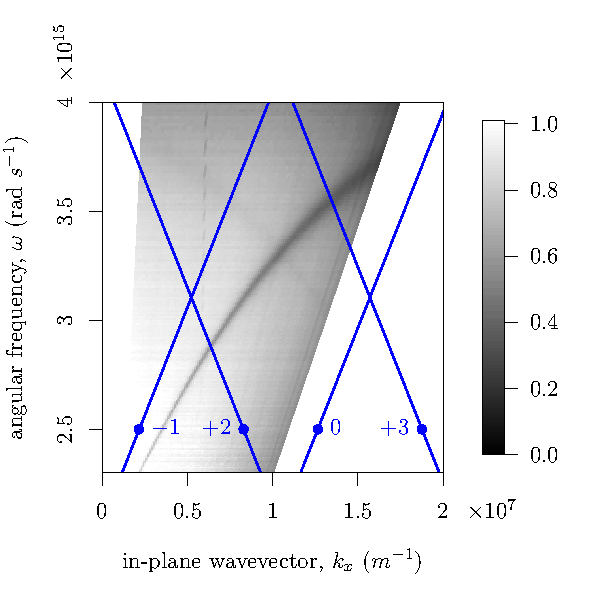
\includegraphics[scale=1]{figure-TEdispersion-symZZ-Exp}
\caption{Experimental data of TE polarized reflectivity as a function of in-plane wavevector and angular frequency, mapping the SPP dispersion on a zig-zag grating. \color{blue}Blue \color{black} lines show the positions of diffracted light lines scattered by $m\mathbf{k}_{gx}$, where $m = −1, +2, 0, +3$.}
\end{center}
\end{figure}

\begin{figure}
\begin{center}
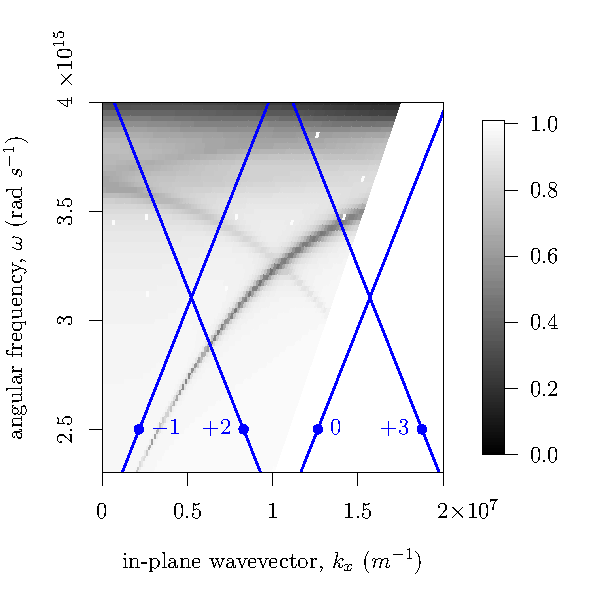
\includegraphics[scale=1]{figure-TEdispersion-symZZ-HFSS}
\caption{Numerical Prediction of the TE polarized reflectivity as a function of in-plane wavevector and angular frequency, mapping the SPP dispersion on a zig-zag grating.\color{blue}Blue \color{black}lines show the positions of diffracted light lines scattered by $m\mathbf{k}_{gx}$, where $m = −1, +2, 0, +3$.}
\end{center}
\end{figure}
Bands of low reflectivity are a result of a resonant excitation of SPPs mapping thereby the dispersion curves of the SPPs. Two Bragg-scattered SPP dispersion curves are observed for this polarization case, one originating at –kgx and one originating at +3kgx. These odd-order diffracted SPs are excited by TE polarized light. The SP dispersion curve from a +2kgx scattering is missing as, on a zig-zag grating, it is not excited by TE polarized light as predicted by equation 2. Using the fitted parameters from figure 2, the dispersion plots were reproduced from FEM modelling and found to be in good agreement and are shown in figure 3. The small difference between the model asymptotic limits of the SPs and experiment may be attributed to the differences between the dielectric function of silver used for the model [17] and our experimental sample. One anticipates that 2kgx diffracted SPPs may be excited by TM polarized light, however the zig-zag surface profile presented does not contain any 2kgx components. Thus for SPPs to gain 2kgx in wavevector they will require two scatterings by kgx a process which, while not forbidden, is inherently weak. To facilitate strong coupling by even-order scattered SPPs and TM polarized light, an even kgx component has to be added to the zig-zag profile, but this removes the mirror symmetry of the grating and the polarization selectivity would be destroyed.





\section{Anisotropic Propagation of SPP modes}

\section{Band-gap character}
\subsection{At normal incidence}
The formation of SPP band-gaps relies on the ability for a propagating SPP mode to Bragg scatter at the BZ boundary and successfully interfere with it's counter-propagating self. Since only diffracted SPPs are observed in the light-cone, the minimum momentum by which a SPP must scatter to meet itself and still be able to couple to light and be observed, is $2k_g$. A SPP scattering by $2k_g$ 
\subsection{At the first BZ}
Normally at Brillouin zone (BZ) boundaries, diffractive coupling results in two counter propagating SPPs, which establish a standing wave [2]. The two standing wave solutions correspond to different field distributions with respect to the grating profile, and between these two energy solutions no surface modes propagate: a SPP band gap forms. However, the dispersion relation shown in figure 3 and the predictions from FEM modelling shows no measurable SPP band gaps at the first BZ
boundaries for this zig-zag grating. Generally, the in-plane wavevector of a standing SPP wave is half that of the total Bragg vector by which the two counter propagating SPPs have been scattered. For the −kgx and +2kgx scattered SPPs, crossing at the first BZ, the SPP wavevector is 3kgx/2. Through symmetry, there are two possible solutions for this standing wave on a zig-zag grating, with the areas of high field of one solution shifted spatially by gx/4 with respect to the other solution. 
\begin{figure}
	\begin{subfigure}[b]{0.5\linewidth}
		\centering% Created by tikzDevice version 0.6.2-92-0ad2792 on 2012-12-18 15:38:44
% !TEX encoding = UTF-8 Unicode
\begin{tikzpicture}[x=1pt,y=1pt]
\definecolor[named]{fillColor}{rgb}{1.00,1.00,1.00}
\path[use as bounding box,fill=fillColor,fill opacity=0.00] (0,0) rectangle (169.83,169.83);
\begin{scope}
\path[clip] ( 30.00, 36.00) rectangle (139.83,145.83);
\definecolor[named]{drawColor}{rgb}{0.00,0.00,0.00}

\path[draw=drawColor,line width= 1.2pt,dash pattern=on 4pt off 4pt ,line join=round,line cap=round] (  0.00, 91.63) --
	(  0.17, 90.92) --
	(  3.25, 77.89) --
	(  6.33, 65.93) --
	(  9.41, 55.98) --
	( 12.50, 48.87) --
	( 15.58, 45.16) --
	( 18.66, 45.16) --
	( 21.74, 48.87) --
	( 24.82, 55.98) --
	( 27.90, 65.93) --
	( 30.99, 77.89) --
	( 34.07, 90.92) --
	( 37.15,103.94) --
	( 40.23,115.91) --
	( 43.31,125.85) --
	( 46.40,132.97) --
	( 49.48,136.67) --
	( 52.56,136.67) --
	( 55.64,132.97) --
	( 58.72,125.85) --
	( 61.80,115.91) --
	( 64.89,103.94) --
	( 67.97, 90.92) --
	( 71.05, 77.89) --
	( 74.13, 65.93) --
	( 77.21, 55.98) --
	( 80.29, 48.87) --
	( 83.38, 45.16) --
	( 86.46, 45.16) --
	( 89.54, 48.87) --
	( 92.62, 55.98) --
	( 95.70, 65.93) --
	( 98.79, 77.89) --
	(101.87, 90.92) --
	(104.95,103.94) --
	(108.03,115.91) --
	(111.11,125.85) --
	(114.19,132.97) --
	(117.28,136.67) --
	(120.36,136.67) --
	(123.44,132.97) --
	(126.52,125.85) --
	(129.60,115.91) --
	(132.68,103.94) --
	(135.77, 90.92) --
	(138.85, 77.89) --
	(141.93, 65.93) --
	(145.01, 55.98) --
	(148.09, 48.87) --
	(151.18, 45.16) --
	(154.26, 45.16) --
	(157.34, 48.87) --
	(160.42, 55.98) --
	(163.50, 65.93) --
	(166.58, 77.89) --
	(169.67, 90.92) --
	(169.83, 91.63);
\end{scope}
\begin{scope}
\path[clip] ( 30.00, 36.00) rectangle (139.83,145.83);
\definecolor[named]{drawColor}{rgb}{0.00,0.00,0.00}

\path[draw=drawColor,line width= 1.2pt,dash pattern=on 4pt off 4pt ,line join=round,line cap=round] (  0.00, 90.21) --
	(  0.17, 90.92) --
	(  3.25,103.94) --
	(  6.33,115.91) --
	(  9.41,125.85) --
	( 12.50,132.97) --
	( 15.58,136.67) --
	( 18.66,136.67) --
	( 21.74,132.97) --
	( 24.82,125.85) --
	( 27.90,115.91) --
	( 30.99,103.94) --
	( 34.07, 90.92) --
	( 37.15, 77.89) --
	( 40.23, 65.93) --
	( 43.31, 55.98) --
	( 46.40, 48.87) --
	( 49.48, 45.16) --
	( 52.56, 45.16) --
	( 55.64, 48.87) --
	( 58.72, 55.98) --
	( 61.80, 65.93) --
	( 64.89, 77.89) --
	( 67.97, 90.92) --
	( 71.05,103.94) --
	( 74.13,115.91) --
	( 77.21,125.85) --
	( 80.29,132.97) --
	( 83.38,136.67) --
	( 86.46,136.67) --
	( 89.54,132.97) --
	( 92.62,125.85) --
	( 95.70,115.91) --
	( 98.79,103.94) --
	(101.87, 90.92) --
	(104.95, 77.89) --
	(108.03, 65.93) --
	(111.11, 55.98) --
	(114.19, 48.87) --
	(117.28, 45.16) --
	(120.36, 45.16) --
	(123.44, 48.87) --
	(126.52, 55.98) --
	(129.60, 65.93) --
	(132.68, 77.89) --
	(135.77, 90.92) --
	(138.85,103.94) --
	(141.93,115.91) --
	(145.01,125.85) --
	(148.09,132.97) --
	(151.18,136.67) --
	(154.26,136.67) --
	(157.34,132.97) --
	(160.42,125.85) --
	(163.50,115.91) --
	(166.58,103.94) --
	(169.67, 90.92) --
	(169.83, 90.21);

\path[draw=drawColor,line width= 0.4pt,line join=round,line cap=round] ( 10.74,128.91) -- ( 18.50,136.67);

\path[draw=drawColor,line width= 0.4pt,line join=round,line cap=round] (  7.13,118.49) -- ( 21.68,133.04);

\path[draw=drawColor,line width= 0.4pt,line join=round,line cap=round] (  4.59,109.13) -- ( 23.76,128.31);

\path[draw=drawColor,line width= 0.4pt,line join=round,line cap=round] (  2.33,100.06) -- ( 25.60,123.33);

\path[draw=drawColor,line width= 0.4pt,line join=round,line cap=round] (  0.00, 90.92) -- (  0.14, 91.05);

\path[draw=drawColor,line width= 0.4pt,line join=round,line cap=round] (  0.22, 91.14) -- ( 27.22,118.13);

\path[draw=drawColor,line width= 0.4pt,line join=round,line cap=round] (  1.44, 85.54) -- (  6.81, 90.92);

\path[draw=drawColor,line width= 0.4pt,line join=round,line cap=round] (  6.81, 90.92) -- ( 28.70,112.81);

\path[draw=drawColor,line width= 0.4pt,line join=round,line cap=round] ( 44.51,128.61) -- ( 52.56,136.67);

\path[draw=drawColor,line width= 0.4pt,line join=round,line cap=round] (  2.74, 80.03) -- ( 13.63, 90.92);

\path[draw=drawColor,line width= 0.4pt,line join=round,line cap=round] ( 13.63, 90.92) -- ( 30.10,107.39);

\path[draw=drawColor,line width= 0.4pt,line join=round,line cap=round] ( 40.96,118.25) -- ( 55.65,132.94);

\path[draw=drawColor,line width= 0.4pt,line join=round,line cap=round] (  4.10, 74.58) -- ( 20.44, 90.92);

\path[draw=drawColor,line width= 0.4pt,line join=round,line cap=round] ( 20.44, 90.92) -- ( 31.46,101.94);

\path[draw=drawColor,line width= 0.4pt,line join=round,line cap=round] ( 38.43,108.90) -- ( 57.71,128.19);

\path[draw=drawColor,line width= 0.4pt,line join=round,line cap=round] (  5.50, 69.16) -- ( 27.25, 90.92);

\path[draw=drawColor,line width= 0.4pt,line join=round,line cap=round] ( 27.25, 90.92) -- ( 32.76, 96.43);

\path[draw=drawColor,line width= 0.4pt,line join=round,line cap=round] ( 36.18, 99.84) -- ( 59.54,123.21);

\path[draw=drawColor,line width= 0.4pt,line join=round,line cap=round] (  6.98, 63.83) -- ( 34.07, 90.92);

\path[draw=drawColor,line width= 0.4pt,line join=round,line cap=round] ( 34.07, 90.92) -- ( 34.07, 90.92);

\path[draw=drawColor,line width= 0.4pt,line join=round,line cap=round] ( 34.07, 90.92) -- ( 61.15,118.00);

\path[draw=drawColor,line width= 0.4pt,line join=round,line cap=round] (  8.59, 58.63) -- ( 31.96, 81.99);

\path[draw=drawColor,line width= 0.4pt,line join=round,line cap=round] ( 35.37, 85.41) -- ( 40.88, 90.92);

\path[draw=drawColor,line width= 0.4pt,line join=round,line cap=round] ( 40.88, 90.92) -- ( 62.64,112.67);

\path[draw=drawColor,line width= 0.4pt,line join=round,line cap=round] ( 78.28,128.32) -- ( 86.54,136.58);

\path[draw=drawColor,line width= 0.4pt,line join=round,line cap=round] ( 10.43, 53.65) -- ( 29.71, 72.93);

\path[draw=drawColor,line width= 0.4pt,line join=round,line cap=round] ( 36.68, 79.90) -- ( 47.70, 90.92);

\path[draw=drawColor,line width= 0.4pt,line join=round,line cap=round] ( 47.70, 90.92) -- ( 64.03,107.25);

\path[draw=drawColor,line width= 0.4pt,line join=round,line cap=round] ( 74.78,118.00) -- ( 89.60,132.82);

\path[draw=drawColor,line width= 0.4pt,line join=round,line cap=round] ( 12.48, 48.89) -- ( 27.18, 63.59);

\path[draw=drawColor,line width= 0.4pt,line join=round,line cap=round] ( 38.04, 74.45) -- ( 54.51, 90.92);

\path[draw=drawColor,line width= 0.4pt,line join=round,line cap=round] ( 54.51, 90.92) -- ( 65.39,101.80);

\path[draw=drawColor,line width= 0.4pt,line join=round,line cap=round] ( 72.27,108.68) -- ( 91.66,128.07);

\path[draw=drawColor,line width= 0.4pt,line join=round,line cap=round] ( 15.57, 45.17) -- ( 23.63, 53.22);

\path[draw=drawColor,line width= 0.4pt,line join=round,line cap=round] ( 39.43, 69.03) -- ( 61.32, 90.92);

\path[draw=drawColor,line width= 0.4pt,line join=round,line cap=round] ( 61.32, 90.92) -- ( 66.70, 96.29);

\path[draw=drawColor,line width= 0.4pt,line join=round,line cap=round] ( 70.03, 99.62) -- ( 93.48,123.08);

\path[draw=drawColor,line width= 0.4pt,line join=round,line cap=round] ( 40.92, 63.70) -- ( 67.92, 90.70);

\path[draw=drawColor,line width= 0.4pt,line join=round,line cap=round] ( 68.00, 90.78) -- ( 68.14, 90.92);

\path[draw=drawColor,line width= 0.4pt,line join=round,line cap=round] ( 68.14, 90.92) -- ( 95.09,117.88);

\path[draw=drawColor,line width= 0.4pt,line join=round,line cap=round] ( 42.53, 58.50) -- ( 65.80, 81.77);

\path[draw=drawColor,line width= 0.4pt,line join=round,line cap=round] ( 69.30, 85.27) -- ( 74.95, 90.92);

\path[draw=drawColor,line width= 0.4pt,line join=round,line cap=round] ( 74.95, 90.92) -- ( 96.57,112.54);

\path[draw=drawColor,line width= 0.4pt,line join=round,line cap=round] (112.05,128.02) -- (120.52,136.48);

\path[draw=drawColor,line width= 0.4pt,line join=round,line cap=round] ( 44.38, 53.53) -- ( 63.55, 72.70);

\path[draw=drawColor,line width= 0.4pt,line join=round,line cap=round] ( 70.61, 79.76) -- ( 81.76, 90.92);

\path[draw=drawColor,line width= 0.4pt,line join=round,line cap=round] ( 81.76, 90.92) -- ( 97.97,107.12);

\path[draw=drawColor,line width= 0.4pt,line join=round,line cap=round] (108.60,117.76) -- (123.55,132.71);

\path[draw=drawColor,line width= 0.4pt,line join=round,line cap=round] ( 46.46, 48.80) -- ( 61.00, 63.34);

\path[draw=drawColor,line width= 0.4pt,line join=round,line cap=round] ( 71.97, 74.31) -- ( 88.58, 90.92);

\path[draw=drawColor,line width= 0.4pt,line join=round,line cap=round] ( 88.58, 90.92) -- ( 99.32,101.66);

\path[draw=drawColor,line width= 0.4pt,line join=round,line cap=round] (106.11,108.45) -- (125.61,127.95);

\path[draw=drawColor,line width= 0.4pt,line join=round,line cap=round] ( 49.63, 45.16) -- ( 57.40, 52.92);

\path[draw=drawColor,line width= 0.4pt,line join=round,line cap=round] ( 73.37, 68.89) -- ( 95.39, 90.92);

\path[draw=drawColor,line width= 0.4pt,line join=round,line cap=round] ( 95.39, 90.92) -- (100.63, 96.15);

\path[draw=drawColor,line width= 0.4pt,line join=round,line cap=round] (103.87, 99.40) -- (127.42,122.95);

\path[draw=drawColor,line width= 0.4pt,line join=round,line cap=round] ( 74.86, 63.57) -- (101.76, 90.47);

\path[draw=drawColor,line width= 0.4pt,line join=round,line cap=round] (101.93, 90.64) -- (102.20, 90.92);

\path[draw=drawColor,line width= 0.4pt,line join=round,line cap=round] (102.20, 90.92) -- (129.03,117.75);

\path[draw=drawColor,line width= 0.4pt,line join=round,line cap=round] ( 76.47, 58.37) -- ( 99.65, 81.55);

\path[draw=drawColor,line width= 0.4pt,line join=round,line cap=round] (103.24, 85.13) -- (109.02, 90.92);

\path[draw=drawColor,line width= 0.4pt,line join=round,line cap=round] (109.02, 90.92) -- (130.51,112.40);

\path[draw=drawColor,line width= 0.4pt,line join=round,line cap=round] (145.82,127.72) -- (154.49,136.39);

\path[draw=drawColor,line width= 0.4pt,line join=round,line cap=round] ( 78.33, 53.41) -- ( 97.39, 72.48);

\path[draw=drawColor,line width= 0.4pt,line join=round,line cap=round] (104.54, 79.62) -- (115.83, 90.92);

\path[draw=drawColor,line width= 0.4pt,line join=round,line cap=round] (115.83, 90.92) -- (131.90,106.99);

\path[draw=drawColor,line width= 0.4pt,line join=round,line cap=round] (142.43,117.51) -- (157.50,132.59);

\path[draw=drawColor,line width= 0.4pt,line join=round,line cap=round] ( 80.43, 48.70) -- ( 94.83, 63.10);

\path[draw=drawColor,line width= 0.4pt,line join=round,line cap=round] (105.91, 74.18) -- (122.65, 90.92);

\path[draw=drawColor,line width= 0.4pt,line join=round,line cap=round] (122.65, 90.92) -- (133.26,101.53);

\path[draw=drawColor,line width= 0.4pt,line join=round,line cap=round] (139.95,108.22) -- (159.56,127.83);

\path[draw=drawColor,line width= 0.4pt,line join=round,line cap=round] ( 83.70, 45.16) -- ( 91.17, 52.63);

\path[draw=drawColor,line width= 0.4pt,line join=round,line cap=round] (107.30, 68.76) -- (129.46, 90.92);

\path[draw=drawColor,line width= 0.4pt,line join=round,line cap=round] (129.46, 90.92) -- (134.56, 96.02);

\path[draw=drawColor,line width= 0.4pt,line join=round,line cap=round] (137.72, 99.18) -- (161.36,122.82);

\path[draw=drawColor,line width= 0.4pt,line join=round,line cap=round] (108.80, 63.44) -- (135.61, 90.25);

\path[draw=drawColor,line width= 0.4pt,line join=round,line cap=round] (135.86, 90.51) -- (136.27, 90.92);

\path[draw=drawColor,line width= 0.4pt,line join=round,line cap=round] (136.27, 90.92) -- (162.97,117.62);

\path[draw=drawColor,line width= 0.4pt,line join=round,line cap=round] (110.41, 58.24) -- (133.50, 81.33);

\path[draw=drawColor,line width= 0.4pt,line join=round,line cap=round] (137.17, 85.00) -- (143.09, 90.92);

\path[draw=drawColor,line width= 0.4pt,line join=round,line cap=round] (143.09, 90.92) -- (164.44,112.27);

\path[draw=drawColor,line width= 0.4pt,line join=round,line cap=round] (112.28, 53.29) -- (131.23, 72.25);

\path[draw=drawColor,line width= 0.4pt,line join=round,line cap=round] (138.47, 79.49) -- (149.90, 90.92);

\path[draw=drawColor,line width= 0.4pt,line join=round,line cap=round] (149.90, 90.92) -- (165.83,106.85);

\path[draw=drawColor,line width= 0.4pt,line join=round,line cap=round] (114.41, 48.61) -- (128.65, 62.85);

\path[draw=drawColor,line width= 0.4pt,line join=round,line cap=round] (139.84, 74.04) -- (156.71, 90.92);

\path[draw=drawColor,line width= 0.4pt,line join=round,line cap=round] (156.71, 90.92) -- (167.19,101.39);

\path[draw=drawColor,line width= 0.4pt,line join=round,line cap=round] (117.77, 45.16) -- (124.94, 52.33);

\path[draw=drawColor,line width= 0.4pt,line join=round,line cap=round] (141.24, 68.62) -- (163.53, 90.92);

\path[draw=drawColor,line width= 0.4pt,line join=round,line cap=round] (163.53, 90.92) -- (168.49, 95.88);

\path[draw=drawColor,line width= 0.4pt,line join=round,line cap=round] (142.74, 63.31) -- (169.46, 90.03);

\path[draw=drawColor,line width= 0.4pt,line join=round,line cap=round] (169.80, 90.37) -- (169.83, 90.41);

\path[draw=drawColor,line width= 0.4pt,line join=round,line cap=round] (144.35, 58.11) -- (167.34, 81.11);

\path[draw=drawColor,line width= 0.4pt,line join=round,line cap=round] (146.23, 53.18) -- (165.07, 72.02);

\path[draw=drawColor,line width= 0.4pt,line join=round,line cap=round] (148.38, 48.52) -- (162.47, 62.61);

\path[draw=drawColor,line width= 0.4pt,line join=round,line cap=round] (151.84, 45.16) -- (158.71, 52.03);

\path[] (  0.00, 91.63) --
	(  0.17, 90.92) --
	(  3.25, 77.89) --
	(  6.33, 65.93) --
	(  9.41, 55.98) --
	( 12.50, 48.87) --
	( 15.58, 45.16) --
	( 18.66, 45.16) --
	( 21.74, 48.87) --
	( 24.82, 55.98) --
	( 27.90, 65.93) --
	( 30.99, 77.89) --
	( 34.07, 90.92) --
	( 37.15,103.94) --
	( 40.23,115.91) --
	( 43.31,125.85) --
	( 46.40,132.97) --
	( 49.48,136.67) --
	( 52.56,136.67) --
	( 55.64,132.97) --
	( 58.72,125.85) --
	( 61.80,115.91) --
	( 64.89,103.94) --
	( 67.97, 90.92) --
	( 71.05, 77.89) --
	( 74.13, 65.93) --
	( 77.21, 55.98) --
	( 80.29, 48.87) --
	( 83.38, 45.16) --
	( 86.46, 45.16) --
	( 89.54, 48.87) --
	( 92.62, 55.98) --
	( 95.70, 65.93) --
	( 98.79, 77.89) --
	(101.87, 90.92) --
	(104.95,103.94) --
	(108.03,115.91) --
	(111.11,125.85) --
	(114.19,132.97) --
	(117.28,136.67) --
	(120.36,136.67) --
	(123.44,132.97) --
	(126.52,125.85) --
	(129.60,115.91) --
	(132.68,103.94) --
	(135.77, 90.92) --
	(138.85, 77.89) --
	(141.93, 65.93) --
	(145.01, 55.98) --
	(148.09, 48.87) --
	(151.18, 45.16) --
	(154.26, 45.16) --
	(157.34, 48.87) --
	(160.42, 55.98) --
	(163.50, 65.93) --
	(166.58, 77.89) --
	(169.67, 90.92) --
	(169.83, 91.63);

\path[] (169.83, 90.92) --
	(  0.00, 90.92);

\path[] (  0.00, 90.21) --
	(  0.17, 90.92) --
	(  3.25,103.94) --
	(  6.33,115.91) --
	(  9.41,125.85) --
	( 12.50,132.97) --
	( 15.58,136.67) --
	( 18.66,136.67) --
	( 21.74,132.97) --
	( 24.82,125.85) --
	( 27.90,115.91) --
	( 30.99,103.94) --
	( 34.07, 90.92) --
	( 37.15, 77.89) --
	( 40.23, 65.93) --
	( 43.31, 55.98) --
	( 46.40, 48.87) --
	( 49.48, 45.16) --
	( 52.56, 45.16) --
	( 55.64, 48.87) --
	( 58.72, 55.98) --
	( 61.80, 65.93) --
	( 64.89, 77.89) --
	( 67.97, 90.92) --
	( 71.05,103.94) --
	( 74.13,115.91) --
	( 77.21,125.85) --
	( 80.29,132.97) --
	( 83.38,136.67) --
	( 86.46,136.67) --
	( 89.54,132.97) --
	( 92.62,125.85) --
	( 95.70,115.91) --
	( 98.79,103.94) --
	(101.87, 90.92) --
	(104.95, 77.89) --
	(108.03, 65.93) --
	(111.11, 55.98) --
	(114.19, 48.87) --
	(117.28, 45.16) --
	(120.36, 45.16) --
	(123.44, 48.87) --
	(126.52, 55.98) --
	(129.60, 65.93) --
	(132.68, 77.89) --
	(135.77, 90.92) --
	(138.85,103.94) --
	(141.93,115.91) --
	(145.01,125.85) --
	(148.09,132.97) --
	(151.18,136.67) --
	(154.26,136.67) --
	(157.34,132.97) --
	(160.42,125.85) --
	(163.50,115.91) --
	(166.58,103.94) --
	(169.67, 90.92) --
	(169.83, 90.21);

\path[] (169.83, 90.92) --
	(  0.00, 90.92);
\definecolor[named]{fillColor}{rgb}{1.00,1.00,1.00}

\path[draw=drawColor,line width= 1.2pt,line join=round,line cap=round,fill=fillColor] ( 34.07, 79.36) --
	(  0.00, 87.10) --
	(  0.00,110.22) --
	( 34.07,102.47) --
	( 84.92,114.03) --
	(135.77,102.47) --
	(169.83,110.22) --
	(169.83, 94.85) --
	(135.77, 79.36) --
	( 84.92, 90.92) --
	cycle;
\end{scope}
\begin{scope}
\path[clip] (  0.00,  0.00) rectangle (169.83,169.83);
\definecolor[named]{drawColor}{rgb}{0.00,0.00,0.00}

\path[draw=drawColor,line width= 0.4pt,line join=round,line cap=round] ( 34.07, 36.00) -- (135.77, 36.00);

\path[draw=drawColor,line width= 0.4pt,line join=round,line cap=round] ( 34.07, 36.00) -- ( 34.07, 30.00);

\path[draw=drawColor,line width= 0.4pt,line join=round,line cap=round] ( 84.92, 36.00) -- ( 84.92, 30.00);

\path[draw=drawColor,line width= 0.4pt,line join=round,line cap=round] (135.77, 36.00) -- (135.77, 30.00);

\node[text=drawColor,anchor=base,inner sep=0pt, outer sep=0pt, scale=  1.00] at ( 34.07, 14.40) {$-\frac{\lambda_{gx}}{2}$};

\node[text=drawColor,anchor=base,inner sep=0pt, outer sep=0pt, scale=  1.00] at ( 84.92, 14.40) {$0$};

\node[text=drawColor,anchor=base,inner sep=0pt, outer sep=0pt, scale=  1.00] at (135.77, 14.40) {$+\frac{\lambda_{gx}}{2}$};

\path[draw=drawColor,line width= 0.4pt,line join=round,line cap=round] ( 34.07,145.83) -- (135.77,145.83);

\path[draw=drawColor,line width= 0.4pt,line join=round,line cap=round] ( 34.07,145.83) -- ( 34.07,151.83);

\path[draw=drawColor,line width= 0.4pt,line join=round,line cap=round] ( 84.92,145.83) -- ( 84.92,151.83);

\path[draw=drawColor,line width= 0.4pt,line join=round,line cap=round] (135.77,145.83) -- (135.77,151.83);
\end{scope}
\begin{scope}
\path[clip] ( 30.00, 36.00) rectangle (139.83,145.83);
\definecolor[named]{drawColor}{rgb}{0.00,0.00,0.00}

\path[draw=drawColor,line width= 0.8pt,dash pattern=on 4pt off 4pt ,line join=round,line cap=round] ( 34.07,  0.00) --
	( 34.07,169.83);

\path[draw=drawColor,line width= 0.8pt,dash pattern=on 4pt off 4pt ,line join=round,line cap=round] (135.77,  0.00) --
	(135.77,169.83);

\path[draw=drawColor,line width= 0.8pt,dash pattern=on 4pt off 4pt ,line join=round,line cap=round] ( 84.92,  0.00) --
	( 84.92,169.83);
\end{scope}
\end{tikzpicture}

		\centering\subcaption{}
	\end{subfigure}
	%
	\begin{subfigure}[b]{0.5\linewidth}
		\centering% Created by tikzDevice version 0.6.2-92-0ad2792 on 2012-12-18 15:38:44
% !TEX encoding = UTF-8 Unicode
\begin{tikzpicture}[x=1pt,y=1pt]
\definecolor[named]{fillColor}{rgb}{1.00,1.00,1.00}
\path[use as bounding box,fill=fillColor,fill opacity=0.00] (0,0) rectangle (169.83,169.83);
\begin{scope}
\path[clip] ( 30.00, 36.00) rectangle (139.83,145.83);
\definecolor[named]{drawColor}{rgb}{0.00,0.00,0.00}

\path[draw=drawColor,line width= 1.2pt,dash pattern=on 4pt off 4pt ,line join=round,line cap=round] (  0.00, 44.79) --
	(  0.17, 44.69) --
	(  3.25, 46.56) --
	(  6.33, 52.03) --
	(  9.41, 60.65) --
	( 12.50, 71.71) --
	( 15.58, 84.34) --
	( 18.66, 97.50) --
	( 21.74,110.12) --
	( 24.82,121.19) --
	( 27.90,129.81) --
	( 30.99,135.27) --
	( 34.07,137.14) --
	( 37.15,135.27) --
	( 40.23,129.81) --
	( 43.31,121.19) --
	( 46.40,110.12) --
	( 49.48, 97.50) --
	( 52.56, 84.34) --
	( 55.64, 71.71) --
	( 58.72, 60.65) --
	( 61.80, 52.03) --
	( 64.89, 46.56) --
	( 67.97, 44.69) --
	( 71.05, 46.56) --
	( 74.13, 52.03) --
	( 77.21, 60.65) --
	( 80.29, 71.71) --
	( 83.38, 84.34) --
	( 86.46, 97.50) --
	( 89.54,110.12) --
	( 92.62,121.19) --
	( 95.70,129.81) --
	( 98.79,135.27) --
	(101.87,137.14) --
	(104.95,135.27) --
	(108.03,129.81) --
	(111.11,121.19) --
	(114.19,110.12) --
	(117.28, 97.50) --
	(120.36, 84.34) --
	(123.44, 71.71) --
	(126.52, 60.65) --
	(129.60, 52.03) --
	(132.68, 46.56) --
	(135.77, 44.69) --
	(138.85, 46.56) --
	(141.93, 52.03) --
	(145.01, 60.65) --
	(148.09, 71.71) --
	(151.18, 84.34) --
	(154.26, 97.50) --
	(157.34,110.12) --
	(160.42,121.19) --
	(163.50,129.81) --
	(166.58,135.27) --
	(169.67,137.14) --
	(169.83,137.04);
\end{scope}
\begin{scope}
\path[clip] ( 30.00, 36.00) rectangle (139.83,145.83);
\definecolor[named]{drawColor}{rgb}{0.00,0.00,0.00}

\path[draw=drawColor,line width= 1.2pt,dash pattern=on 4pt off 4pt ,line join=round,line cap=round] (  0.00,137.04) --
	(  0.17,137.14) --
	(  3.25,135.27) --
	(  6.33,129.81) --
	(  9.41,121.19) --
	( 12.50,110.12) --
	( 15.58, 97.50) --
	( 18.66, 84.34) --
	( 21.74, 71.71) --
	( 24.82, 60.65) --
	( 27.90, 52.03) --
	( 30.99, 46.56) --
	( 34.07, 44.69) --
	( 37.15, 46.56) --
	( 40.23, 52.03) --
	( 43.31, 60.65) --
	( 46.40, 71.71) --
	( 49.48, 84.34) --
	( 52.56, 97.50) --
	( 55.64,110.12) --
	( 58.72,121.19) --
	( 61.80,129.81) --
	( 64.89,135.27) --
	( 67.97,137.14) --
	( 71.05,135.27) --
	( 74.13,129.81) --
	( 77.21,121.19) --
	( 80.29,110.12) --
	( 83.38, 97.50) --
	( 86.46, 84.34) --
	( 89.54, 71.71) --
	( 92.62, 60.65) --
	( 95.70, 52.03) --
	( 98.79, 46.56) --
	(101.87, 44.69) --
	(104.95, 46.56) --
	(108.03, 52.03) --
	(111.11, 60.65) --
	(114.19, 71.71) --
	(117.28, 84.34) --
	(120.36, 97.50) --
	(123.44,110.12) --
	(126.52,121.19) --
	(129.60,129.81) --
	(132.68,135.27) --
	(135.77,137.14) --
	(138.85,135.27) --
	(141.93,129.81) --
	(145.01,121.19) --
	(148.09,110.12) --
	(151.18, 97.50) --
	(154.26, 84.34) --
	(157.34, 71.71) --
	(160.42, 60.65) --
	(163.50, 52.03) --
	(166.58, 46.56) --
	(169.67, 44.69) --
	(169.83, 44.79);

\path[draw=drawColor,line width= 0.4pt,line join=round,line cap=round] (  0.00,131.80) -- (  3.15,134.95);

\path[draw=drawColor,line width= 0.4pt,line join=round,line cap=round] (  0.00,124.99) -- (  5.76,130.74);

\path[draw=drawColor,line width= 0.4pt,line join=round,line cap=round] (  0.00,118.17) -- (  7.81,125.99);

\path[draw=drawColor,line width= 0.4pt,line join=round,line cap=round] (  0.00,111.36) -- (  9.44,120.80);

\path[draw=drawColor,line width= 0.4pt,line join=round,line cap=round] (  0.00,104.55) -- ( 11.04,115.58);

\path[draw=drawColor,line width= 0.4pt,line join=round,line cap=round] (  0.00, 97.73) -- ( 12.43,110.17);

\path[draw=drawColor,line width= 0.4pt,line join=round,line cap=round] ( 25.57,123.31) -- ( 37.12,134.85);

\path[draw=drawColor,line width= 0.4pt,line join=round,line cap=round] (  0.00, 90.92) -- ( 13.83,104.75);

\path[draw=drawColor,line width= 0.4pt,line join=round,line cap=round] ( 22.69,113.61) -- ( 39.71,130.62);

\path[draw=drawColor,line width= 0.4pt,line join=round,line cap=round] (  0.00, 84.10) -- (  6.81, 90.92);

\path[draw=drawColor,line width= 0.4pt,line join=round,line cap=round] (  6.81, 90.92) -- ( 15.15, 99.25);

\path[draw=drawColor,line width= 0.4pt,line join=round,line cap=round] ( 20.33,104.43) -- ( 41.77,125.87);

\path[draw=drawColor,line width= 0.4pt,line join=round,line cap=round] (  0.00, 77.29) -- ( 13.63, 90.92);

\path[draw=drawColor,line width= 0.4pt,line join=round,line cap=round] ( 13.63, 90.92) -- ( 16.45, 93.74);

\path[draw=drawColor,line width= 0.4pt,line join=round,line cap=round] ( 18.20, 95.49) -- ( 43.38,120.67);

\path[draw=drawColor,line width= 0.4pt,line join=round,line cap=round] (  0.00, 70.48) -- ( 16.09, 86.56);

\path[draw=drawColor,line width= 0.4pt,line join=round,line cap=round] ( 17.75, 88.23) -- ( 20.44, 90.92);

\path[draw=drawColor,line width= 0.4pt,line join=round,line cap=round] ( 20.44, 90.92) -- ( 44.97,115.45);

\path[draw=drawColor,line width= 0.4pt,line join=round,line cap=round] (  0.00, 63.66) -- ( 13.97, 77.63);

\path[draw=drawColor,line width= 0.4pt,line join=round,line cap=round] ( 19.06, 82.72) -- ( 27.25, 90.92);

\path[draw=drawColor,line width= 0.4pt,line join=round,line cap=round] ( 27.25, 90.92) -- ( 46.37,110.03);

\path[draw=drawColor,line width= 0.4pt,line join=round,line cap=round] ( 59.40,123.06) -- ( 71.10,134.76);

\path[draw=drawColor,line width= 0.4pt,line join=round,line cap=round] (  0.00, 56.85) -- ( 11.61, 68.46);

\path[draw=drawColor,line width= 0.4pt,line join=round,line cap=round] ( 20.37, 77.22) -- ( 34.07, 90.92);

\path[draw=drawColor,line width= 0.4pt,line join=round,line cap=round] ( 34.07, 90.92) -- ( 47.76,104.61);

\path[draw=drawColor,line width= 0.4pt,line join=round,line cap=round] ( 56.53,113.38) -- ( 73.66,130.51);

\path[draw=drawColor,line width= 0.4pt,line join=round,line cap=round] (  0.00, 50.04) -- (  8.74, 58.77);

\path[draw=drawColor,line width= 0.4pt,line join=round,line cap=round] ( 21.77, 71.80) -- ( 40.88, 90.92);

\path[draw=drawColor,line width= 0.4pt,line join=round,line cap=round] ( 40.88, 90.92) -- ( 49.08, 99.11);

\path[draw=drawColor,line width= 0.4pt,line join=round,line cap=round] ( 54.17,104.20) -- ( 75.71,125.74);

\path[draw=drawColor,line width= 0.4pt,line join=round,line cap=round] ( 23.16, 66.39) -- ( 47.70, 90.92);

\path[draw=drawColor,line width= 0.4pt,line join=round,line cap=round] ( 47.70, 90.92) -- ( 50.38, 93.60);

\path[draw=drawColor,line width= 0.4pt,line join=round,line cap=round] ( 52.05, 95.27) -- ( 77.32,120.54);

\path[draw=drawColor,line width= 0.4pt,line join=round,line cap=round] ( 24.76, 61.17) -- ( 49.94, 86.34);

\path[draw=drawColor,line width= 0.4pt,line join=round,line cap=round] ( 51.69, 88.09) -- ( 54.51, 90.92);

\path[draw=drawColor,line width= 0.4pt,line join=round,line cap=round] ( 54.51, 90.92) -- ( 78.91,115.31);

\path[draw=drawColor,line width= 0.4pt,line join=round,line cap=round] ( 26.37, 55.97) -- ( 47.81, 77.40);

\path[draw=drawColor,line width= 0.4pt,line join=round,line cap=round] ( 52.99, 82.58) -- ( 61.32, 90.92);

\path[draw=drawColor,line width= 0.4pt,line join=round,line cap=round] ( 61.32, 90.92) -- ( 80.30,109.90);

\path[draw=drawColor,line width= 0.4pt,line join=round,line cap=round] ( 93.22,122.82) -- (105.07,134.67);

\path[draw=drawColor,line width= 0.4pt,line join=round,line cap=round] ( 28.43, 51.21) -- ( 45.45, 68.23);

\path[draw=drawColor,line width= 0.4pt,line join=round,line cap=round] ( 54.31, 77.09) -- ( 68.14, 90.92);

\path[draw=drawColor,line width= 0.4pt,line join=round,line cap=round] ( 68.14, 90.92) -- ( 81.70,104.48);

\path[draw=drawColor,line width= 0.4pt,line join=round,line cap=round] ( 90.37,113.15) -- (107.61,130.39);

\path[draw=drawColor,line width= 0.4pt,line join=round,line cap=round] ( 31.01, 46.98) -- ( 42.56, 58.53);

\path[draw=drawColor,line width= 0.4pt,line join=round,line cap=round] ( 55.70, 71.67) -- ( 74.95, 90.92);

\path[draw=drawColor,line width= 0.4pt,line join=round,line cap=round] ( 74.95, 90.92) -- ( 83.01, 98.98);

\path[draw=drawColor,line width= 0.4pt,line join=round,line cap=round] ( 88.01,103.98) -- (109.65,125.61);

\path[draw=drawColor,line width= 0.4pt,line join=round,line cap=round] ( 57.10, 66.25) -- ( 81.76, 90.92);

\path[draw=drawColor,line width= 0.4pt,line join=round,line cap=round] ( 81.76, 90.92) -- ( 84.31, 93.47);

\path[draw=drawColor,line width= 0.4pt,line join=round,line cap=round] ( 85.89, 95.05) -- (111.26,120.41);

\path[draw=drawColor,line width= 0.4pt,line join=round,line cap=round] ( 58.70, 61.04) -- ( 83.78, 86.12);

\path[draw=drawColor,line width= 0.4pt,line join=round,line cap=round] ( 85.62, 87.96) -- ( 88.58, 90.92);

\path[draw=drawColor,line width= 0.4pt,line join=round,line cap=round] ( 88.58, 90.92) -- (112.84,115.18);

\path[draw=drawColor,line width= 0.4pt,line join=round,line cap=round] (133.69,136.03) -- (134.33,136.67);

\path[draw=drawColor,line width= 0.4pt,line join=round,line cap=round] ( 60.32, 55.85) -- ( 81.65, 77.18);

\path[draw=drawColor,line width= 0.4pt,line join=round,line cap=round] ( 86.92, 82.45) -- ( 95.39, 90.92);

\path[draw=drawColor,line width= 0.4pt,line join=round,line cap=round] ( 95.39, 90.92) -- (114.24,109.76);

\path[draw=drawColor,line width= 0.4pt,line join=round,line cap=round] (127.05,122.57) -- (139.05,134.58);

\path[draw=drawColor,line width= 0.4pt,line join=round,line cap=round] ( 62.38, 51.09) -- ( 79.29, 68.00);

\path[draw=drawColor,line width= 0.4pt,line join=round,line cap=round] ( 88.24, 76.95) -- (102.20, 90.92);

\path[draw=drawColor,line width= 0.4pt,line join=round,line cap=round] (102.20, 90.92) -- (115.63,104.34);

\path[draw=drawColor,line width= 0.4pt,line join=round,line cap=round] (124.21,112.92) -- (141.56,130.27);

\path[draw=drawColor,line width= 0.4pt,line join=round,line cap=round] ( 64.99, 46.89) -- ( 76.39, 58.28);

\path[draw=drawColor,line width= 0.4pt,line join=round,line cap=round] ( 89.64, 71.54) -- (109.02, 90.92);

\path[draw=drawColor,line width= 0.4pt,line join=round,line cap=round] (109.02, 90.92) -- (116.94, 98.84);

\path[draw=drawColor,line width= 0.4pt,line join=round,line cap=round] (121.85,103.75) -- (143.59,125.48);

\path[draw=drawColor,line width= 0.4pt,line join=round,line cap=round] ( 91.03, 66.12) -- (115.83, 90.92);

\path[draw=drawColor,line width= 0.4pt,line join=round,line cap=round] (115.83, 90.92) -- (118.25, 93.33);

\path[draw=drawColor,line width= 0.4pt,line join=round,line cap=round] (119.74, 94.83) -- (145.20,120.28);

\path[draw=drawColor,line width= 0.4pt,line join=round,line cap=round] ( 92.64, 60.91) -- (117.63, 85.90);

\path[draw=drawColor,line width= 0.4pt,line join=round,line cap=round] (119.55, 87.82) -- (122.65, 90.92);

\path[draw=drawColor,line width= 0.4pt,line join=round,line cap=round] (122.65, 90.92) -- (146.77,115.05);

\path[draw=drawColor,line width= 0.4pt,line join=round,line cap=round] (166.76,135.03) -- (168.40,136.67);

\path[draw=drawColor,line width= 0.4pt,line join=round,line cap=round] ( 94.27, 55.73) -- (115.49, 76.95);

\path[draw=drawColor,line width= 0.4pt,line join=round,line cap=round] (120.85, 82.31) -- (129.46, 90.92);

\path[draw=drawColor,line width= 0.4pt,line join=round,line cap=round] (129.46, 90.92) -- (148.17,109.63);

\path[draw=drawColor,line width= 0.4pt,line join=round,line cap=round] (160.87,122.33) -- (169.83,131.29);

\path[draw=drawColor,line width= 0.4pt,line join=round,line cap=round] ( 96.33, 50.98) -- (113.13, 67.77);

\path[draw=drawColor,line width= 0.4pt,line join=round,line cap=round] (122.18, 76.82) -- (136.27, 90.92);

\path[draw=drawColor,line width= 0.4pt,line join=round,line cap=round] (136.27, 90.92) -- (149.57,104.21);

\path[draw=drawColor,line width= 0.4pt,line join=round,line cap=round] (158.05,112.70) -- (169.83,124.48);

\path[draw=drawColor,line width= 0.4pt,line join=round,line cap=round] ( 98.97, 46.80) -- (110.21, 58.04);

\path[draw=drawColor,line width= 0.4pt,line join=round,line cap=round] (123.57, 71.40) -- (143.09, 90.92);

\path[draw=drawColor,line width= 0.4pt,line join=round,line cap=round] (143.09, 90.92) -- (150.87, 98.70);

\path[draw=drawColor,line width= 0.4pt,line join=round,line cap=round] (155.70,103.53) -- (169.83,117.66);

\path[draw=drawColor,line width= 0.4pt,line join=round,line cap=round] (124.97, 65.98) -- (149.90, 90.92);

\path[draw=drawColor,line width= 0.4pt,line join=round,line cap=round] (149.90, 90.92) -- (152.18, 93.19);

\path[draw=drawColor,line width= 0.4pt,line join=round,line cap=round] (153.59, 94.61) -- (169.83,110.85);

\path[draw=drawColor,line width= 0.4pt,line join=round,line cap=round] (126.58, 60.78) -- (151.48, 85.68);

\path[draw=drawColor,line width= 0.4pt,line join=round,line cap=round] (153.48, 87.68) -- (156.71, 90.92);

\path[draw=drawColor,line width= 0.4pt,line join=round,line cap=round] (156.71, 90.92) -- (169.83,104.04);

\path[draw=drawColor,line width= 0.4pt,line join=round,line cap=round] (128.22, 55.61) -- (149.33, 76.72);

\path[draw=drawColor,line width= 0.4pt,line join=round,line cap=round] (154.79, 82.17) -- (163.53, 90.92);

\path[draw=drawColor,line width= 0.4pt,line join=round,line cap=round] (163.53, 90.92) -- (169.83, 97.22);

\path[draw=drawColor,line width= 0.4pt,line join=round,line cap=round] (130.28, 50.86) -- (146.97, 67.55);

\path[draw=drawColor,line width= 0.4pt,line join=round,line cap=round] (156.11, 76.69) -- (169.83, 90.41);

\path[draw=drawColor,line width= 0.4pt,line join=round,line cap=round] (132.94, 46.70) -- (144.03, 57.80);

\path[draw=drawColor,line width= 0.4pt,line join=round,line cap=round] (157.50, 71.27) -- (169.83, 83.60);

\path[draw=drawColor,line width= 0.4pt,line join=round,line cap=round] (158.90, 65.85) -- (169.83, 76.78);

\path[draw=drawColor,line width= 0.4pt,line join=round,line cap=round] (160.51, 60.65) -- (169.83, 69.97);

\path[draw=drawColor,line width= 0.4pt,line join=round,line cap=round] (162.17, 55.49) -- (169.83, 63.16);

\path[draw=drawColor,line width= 0.4pt,line join=round,line cap=round] (164.23, 50.74) -- (169.83, 56.34);

\path[draw=drawColor,line width= 0.4pt,line join=round,line cap=round] (166.92, 46.61) -- (169.83, 49.53);

\path[] (  0.00, 45.16) --
	(  1.71, 45.16) --
	(  4.79, 48.87) --
	(  7.87, 55.98) --
	( 10.95, 65.93) --
	( 14.04, 77.89) --
	( 17.12, 90.92) --
	( 20.20,103.94) --
	( 23.28,115.91) --
	( 26.36,125.85) --
	( 29.45,132.97) --
	( 32.53,136.67) --
	( 35.61,136.67) --
	( 38.69,132.97) --
	( 41.77,125.85) --
	( 44.85,115.91) --
	( 47.94,103.94) --
	( 51.02, 90.92) --
	( 54.10, 77.89) --
	( 57.18, 65.93) --
	( 60.26, 55.98) --
	( 63.34, 48.87) --
	( 66.43, 45.16) --
	( 69.51, 45.16) --
	( 72.59, 48.87) --
	( 75.67, 55.98) --
	( 78.75, 65.93) --
	( 81.84, 77.89) --
	( 84.92, 90.92) --
	( 88.00,103.94) --
	( 91.08,115.91) --
	( 94.16,125.85) --
	( 97.24,132.97) --
	(100.33,136.67) --
	(103.41,136.67) --
	(106.49,132.97) --
	(109.57,125.85) --
	(112.65,115.91) --
	(115.74,103.94) --
	(118.82, 90.92) --
	(121.90, 77.89) --
	(124.98, 65.93) --
	(128.06, 55.98) --
	(131.14, 48.87) --
	(134.23, 45.16) --
	(137.31, 45.16) --
	(140.39, 48.87) --
	(143.47, 55.98) --
	(146.55, 65.93) --
	(149.63, 77.89) --
	(152.72, 90.92) --
	(155.80,103.94) --
	(158.88,115.91) --
	(161.96,125.85) --
	(165.04,132.97) --
	(168.13,136.67) --
	(169.83,136.67);

\path[] (169.83, 90.92) --
	(  0.00, 90.92);

\path[] (  0.00,136.67) --
	(  1.71,136.67) --
	(  4.79,132.97) --
	(  7.87,125.85) --
	( 10.95,115.91) --
	( 14.04,103.94) --
	( 17.12, 90.92) --
	( 20.20, 77.89) --
	( 23.28, 65.93) --
	( 26.36, 55.98) --
	( 29.45, 48.87) --
	( 32.53, 45.16) --
	( 35.61, 45.16) --
	( 38.69, 48.87) --
	( 41.77, 55.98) --
	( 44.85, 65.93) --
	( 47.94, 77.89) --
	( 51.02, 90.92) --
	( 54.10,103.94) --
	( 57.18,115.91) --
	( 60.26,125.85) --
	( 63.34,132.97) --
	( 66.43,136.67) --
	( 69.51,136.67) --
	( 72.59,132.97) --
	( 75.67,125.85) --
	( 78.75,115.91) --
	( 81.84,103.94) --
	( 84.92, 90.92) --
	( 88.00, 77.89) --
	( 91.08, 65.93) --
	( 94.16, 55.98) --
	( 97.24, 48.87) --
	(100.33, 45.16) --
	(103.41, 45.16) --
	(106.49, 48.87) --
	(109.57, 55.98) --
	(112.65, 65.93) --
	(115.74, 77.89) --
	(118.82, 90.92) --
	(121.90,103.94) --
	(124.98,115.91) --
	(128.06,125.85) --
	(131.14,132.97) --
	(134.23,136.67) --
	(137.31,136.67) --
	(140.39,132.97) --
	(143.47,125.85) --
	(146.55,115.91) --
	(149.63,103.94) --
	(152.72, 90.92) --
	(155.80, 77.89) --
	(158.88, 65.93) --
	(161.96, 55.98) --
	(165.04, 48.87) --
	(168.13, 45.16) --
	(169.83, 45.16);

\path[] (169.83, 90.92) --
	(  0.00, 90.92);
\definecolor[named]{fillColor}{rgb}{1.00,1.00,1.00}

\path[draw=drawColor,line width= 1.2pt,line join=round,line cap=round,fill=fillColor] ( 34.07, 79.36) --
	(  0.00, 87.10) --
	(  0.00,110.22) --
	( 34.07,102.47) --
	( 84.92,114.03) --
	(135.77,102.47) --
	(169.83,110.22) --
	(169.83, 94.85) --
	(135.77, 79.36) --
	( 84.92, 90.92) --
	cycle;
\end{scope}
\begin{scope}
\path[clip] (  0.00,  0.00) rectangle (169.83,169.83);
\definecolor[named]{drawColor}{rgb}{0.00,0.00,0.00}

\path[draw=drawColor,line width= 0.4pt,line join=round,line cap=round] ( 34.07, 36.00) -- (135.77, 36.00);

\path[draw=drawColor,line width= 0.4pt,line join=round,line cap=round] ( 34.07, 36.00) -- ( 34.07, 30.00);

\path[draw=drawColor,line width= 0.4pt,line join=round,line cap=round] ( 84.92, 36.00) -- ( 84.92, 30.00);

\path[draw=drawColor,line width= 0.4pt,line join=round,line cap=round] (135.77, 36.00) -- (135.77, 30.00);

\node[text=drawColor,anchor=base,inner sep=0pt, outer sep=0pt, scale=  1.00] at ( 34.07, 14.40) {$-\frac{\lambda_{gx}}{2}$};

\node[text=drawColor,anchor=base,inner sep=0pt, outer sep=0pt, scale=  1.00] at ( 84.92, 14.40) {$0$};

\node[text=drawColor,anchor=base,inner sep=0pt, outer sep=0pt, scale=  1.00] at (135.77, 14.40) {$+\frac{\lambda_{gx}}{2}$};

\path[draw=drawColor,line width= 0.4pt,line join=round,line cap=round] ( 34.07,145.83) -- (135.77,145.83);

\path[draw=drawColor,line width= 0.4pt,line join=round,line cap=round] ( 34.07,145.83) -- ( 34.07,151.83);

\path[draw=drawColor,line width= 0.4pt,line join=round,line cap=round] ( 84.92,145.83) -- ( 84.92,151.83);

\path[draw=drawColor,line width= 0.4pt,line join=round,line cap=round] (135.77,145.83) -- (135.77,151.83);
\end{scope}
\begin{scope}
\path[clip] ( 30.00, 36.00) rectangle (139.83,145.83);
\definecolor[named]{drawColor}{rgb}{0.00,0.00,0.00}

\path[draw=drawColor,line width= 0.8pt,dash pattern=on 4pt off 4pt ,line join=round,line cap=round] ( 34.07,  0.00) --
	( 34.07,169.83);

\path[draw=drawColor,line width= 0.8pt,dash pattern=on 4pt off 4pt ,line join=round,line cap=round] (135.77,  0.00) --
	(135.77,169.83);

\path[draw=drawColor,line width= 0.8pt,dash pattern=on 4pt off 4pt ,line join=round,line cap=round] ( 84.92,  0.00) --
	( 84.92,169.83);
\end{scope}
\end{tikzpicture}

		\centering\subcaption{}
	\end{subfigure}
\caption{Cartoon of the two standing wave solutions for SPPs at the $1^{st}$ BZ. Since the peaks and troughs of the zigzag exist equivalent electromagnetic environments, the solutions are degenerate in energy, and no bad-gap forms.}
\end{figure}
Because of the zig-zag reflection symmetry, the arrangements of these two field solutions on the zig-zag surface are equivalent. The solutions are degenerate in energy and therefore no band gaps at the first BZ are observed.
The induced charge sits along the zig-zag. Unlike band-gaps on surface-relief gratings, the charge density for both standing wave solutions sits at potentials that are indistinguishable from one another. The electromagnetic environments for both solutions are indistinguishable and so there can be no energy difference between the two eignestates. For this reason, no band-gap is possible for the $-1$ and $+2$ SPP mode crossing at the first Brillioun Zone.

The equivalence in energy of these two standing wave solutions can be broken by the removal of the zig-zag grating's mirror plane. By asymmetrizing the zig-zag, the electric field arrangements for both possible standing waves differ in energy and a bandgap may form. This is demonstrated in figure \ref{fig:bandgaps}, where finite element method modelling has been used to extract the eigenmodes at the first BZ boundary for three possible unit cell variations of the zig-zag grating. 
Additionally, the removal of the mirror plane nullifies the finding of equation \ref{eq:odd-even-fouriers}, as now the surface pertubation contains both odd and even Fourier components. This allows the excitation of  SPPs with either polarization, as shown in figure \ref{fig:?}. 
\begin{figure}
\centering
\begin{subfigure}[b]{0.3\linewidth}
\centering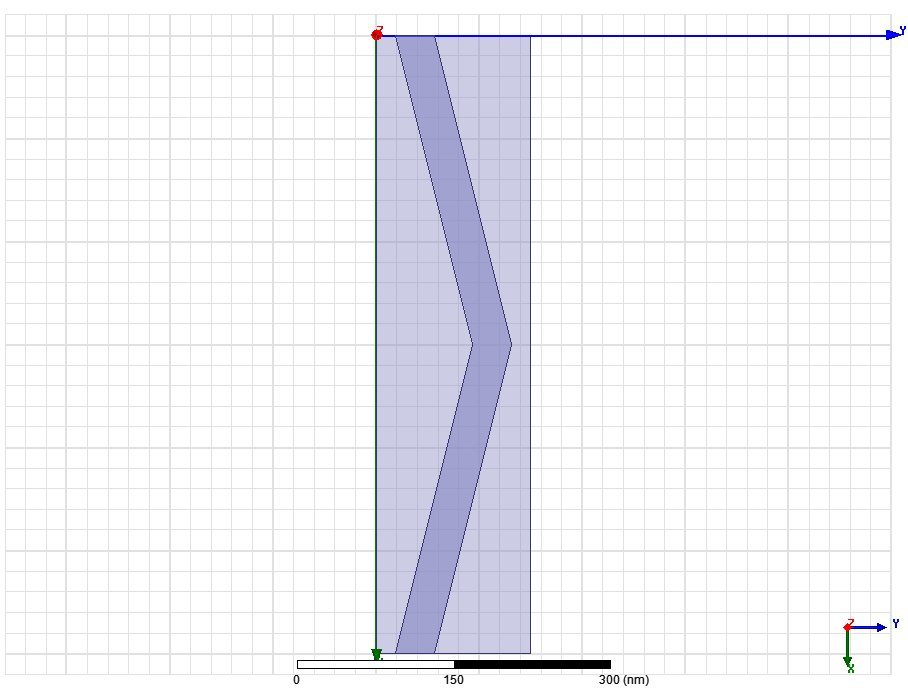
\includegraphics[width=\linewidth]{temp-bandgaps/noOffset.jpg}
\caption{}
\end{subfigure}
\begin{subfigure}[b]{0.3\linewidth}
\centering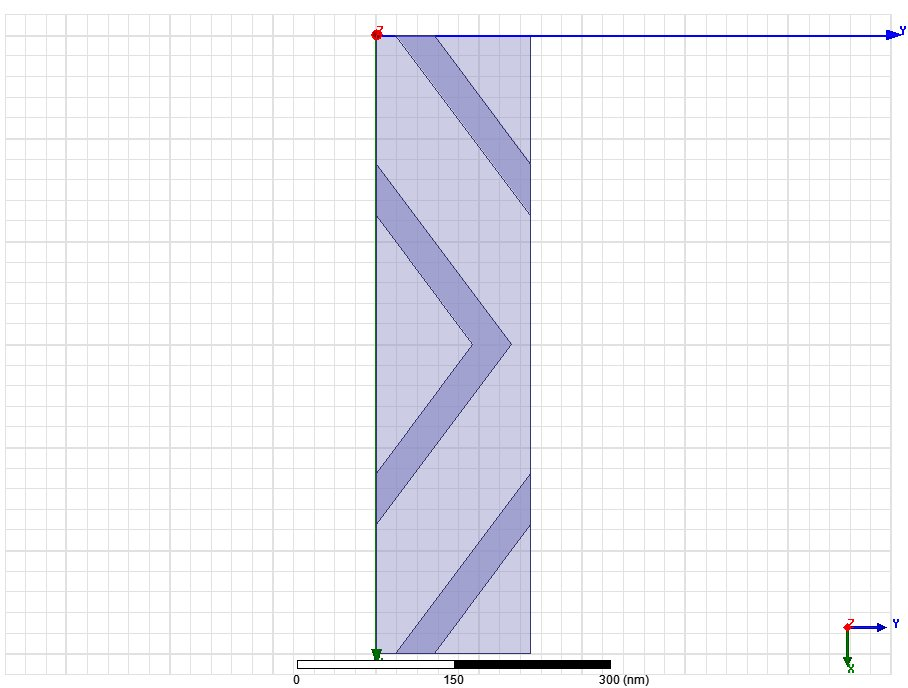
\includegraphics[width=\linewidth]{temp-bandgaps/150yOffset.jpg}
\caption{}
\end{subfigure}
\begin{subfigure}[b]{0.3\linewidth}
\centering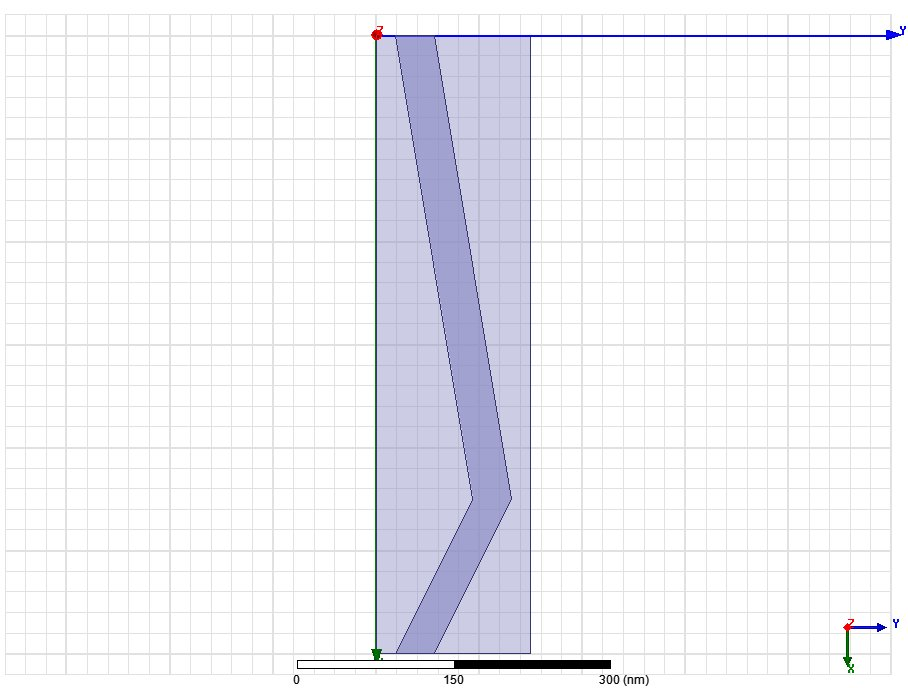
\includegraphics[width=\linewidth]{temp-bandgaps/150xOffset.jpg}
\caption{}
\end{subfigure}

\begin{subfigure}[b]{0.3\linewidth}
\centering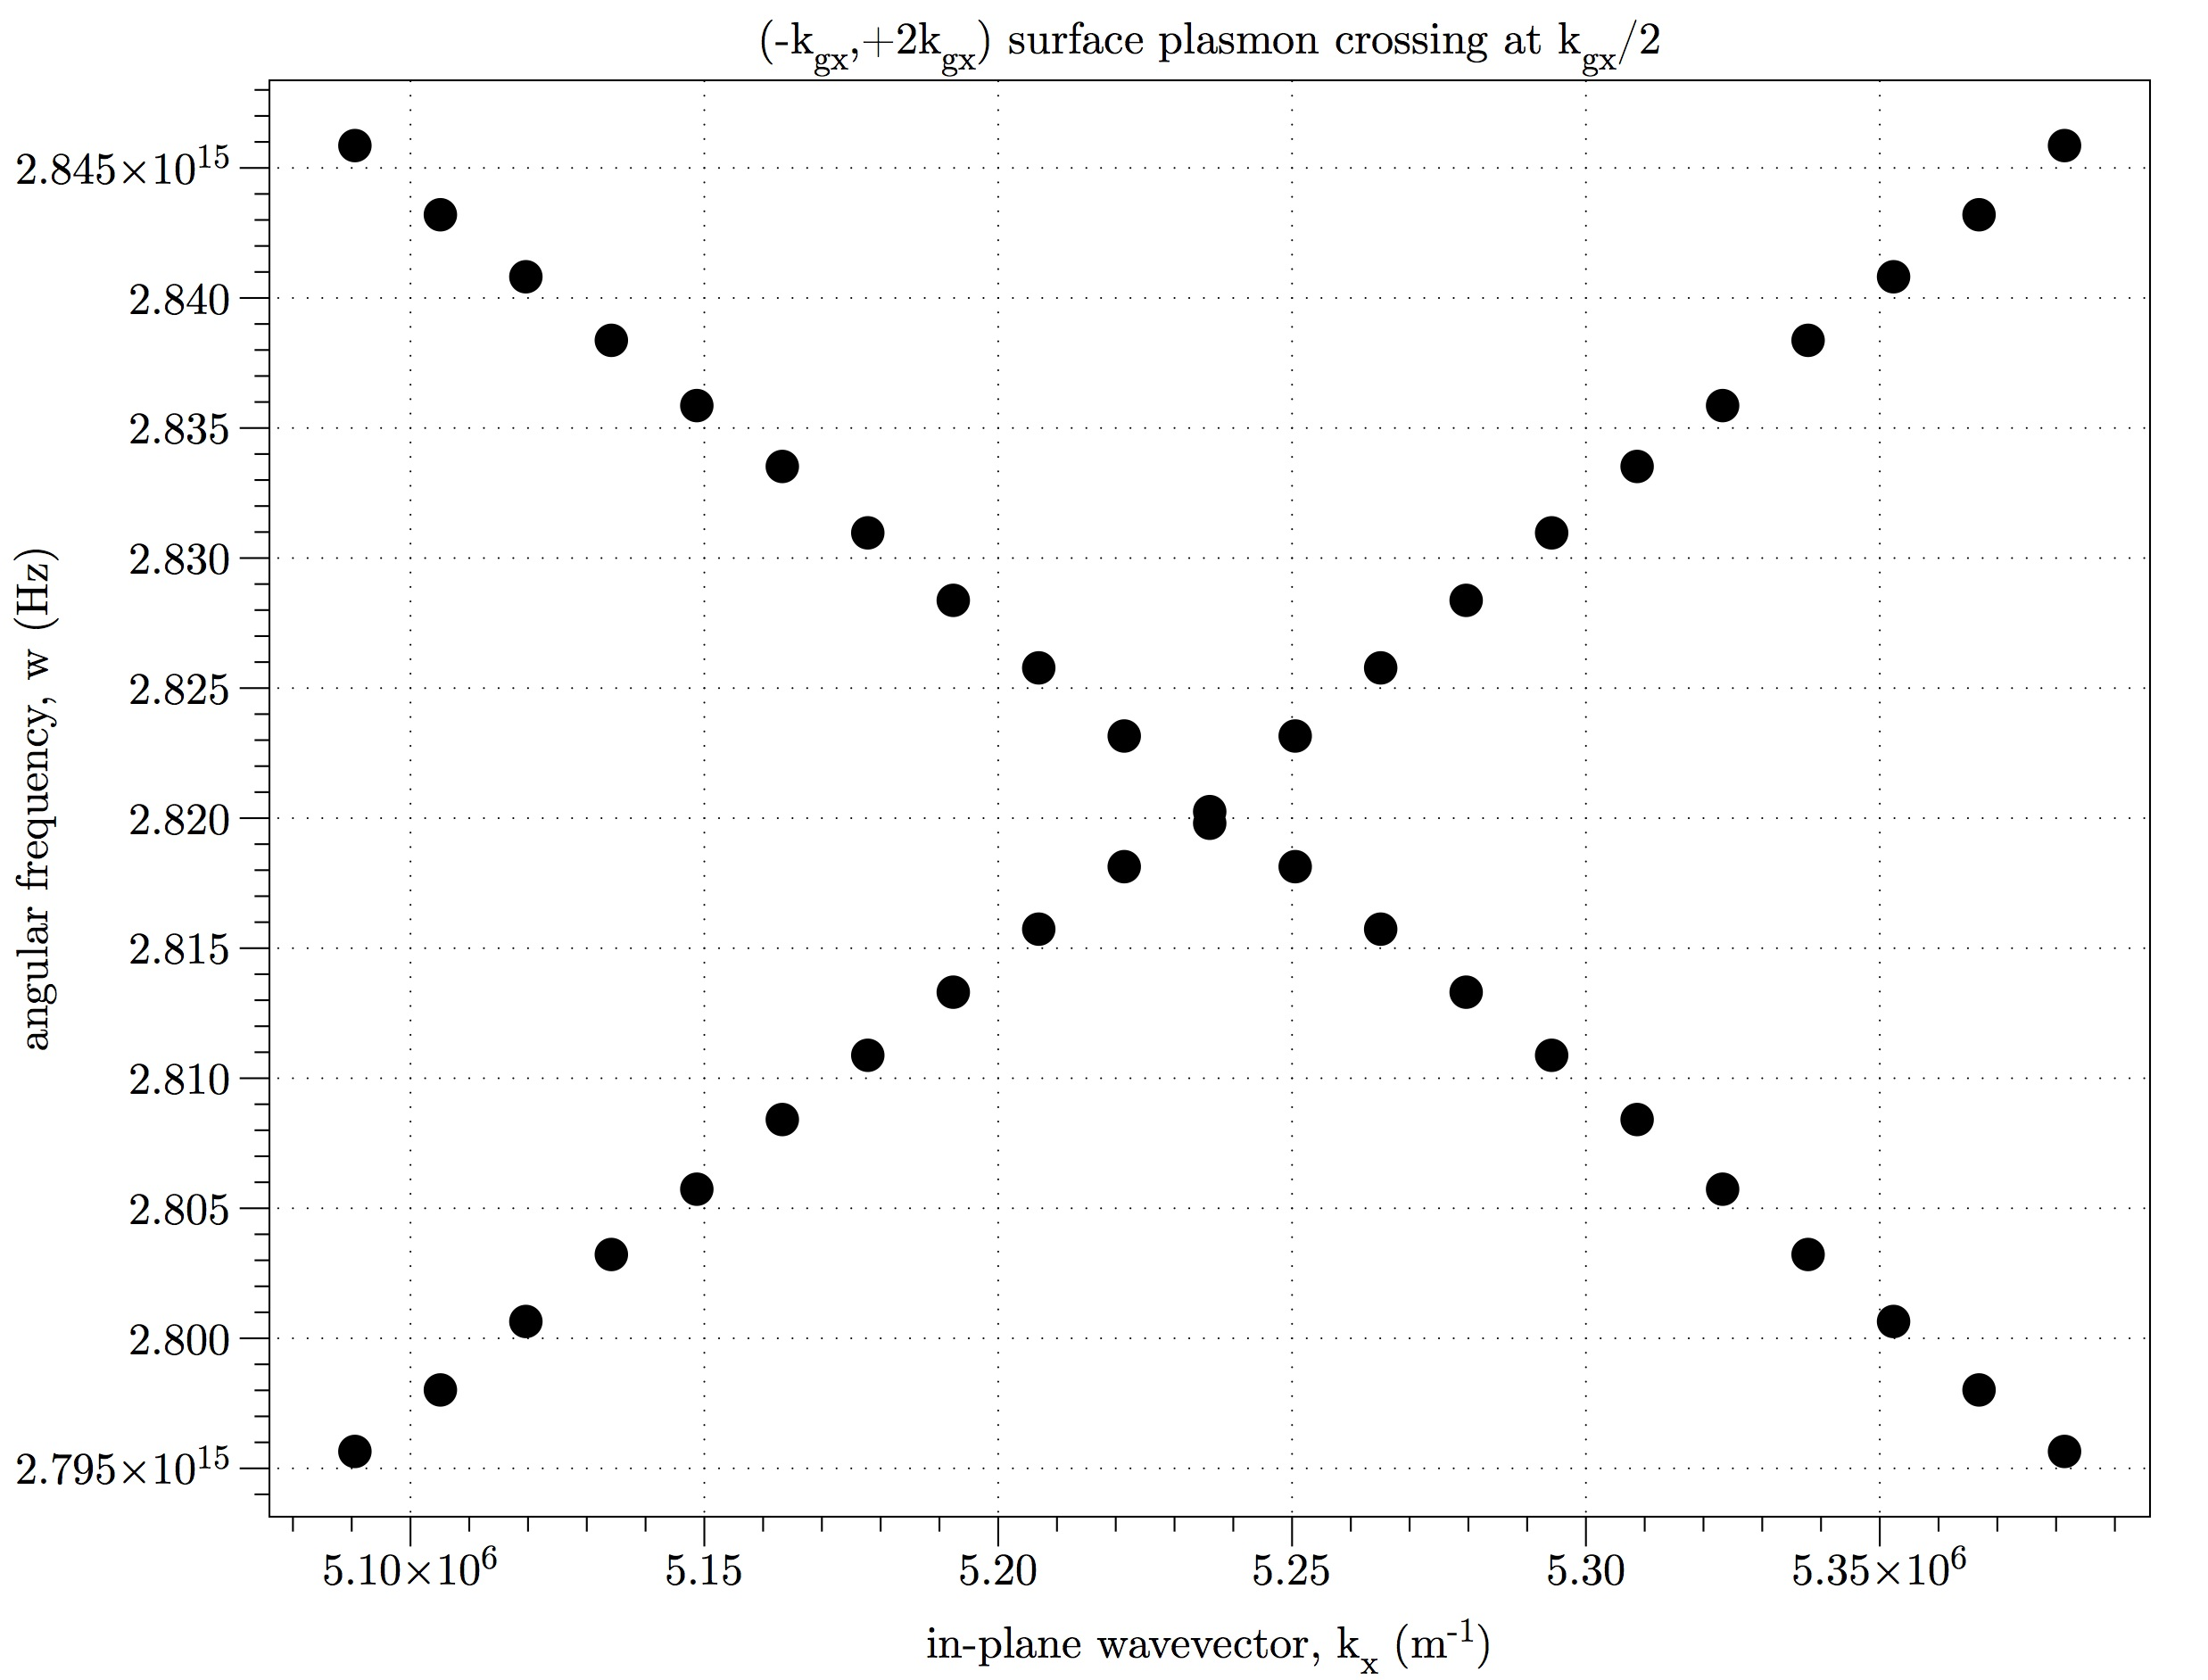
\includegraphics[width=\linewidth]{temp-bandgaps/2kg-kg-0nm-offset.jpg}
\caption{}
\end{subfigure}
\begin{subfigure}[b]{0.3\linewidth}
\centering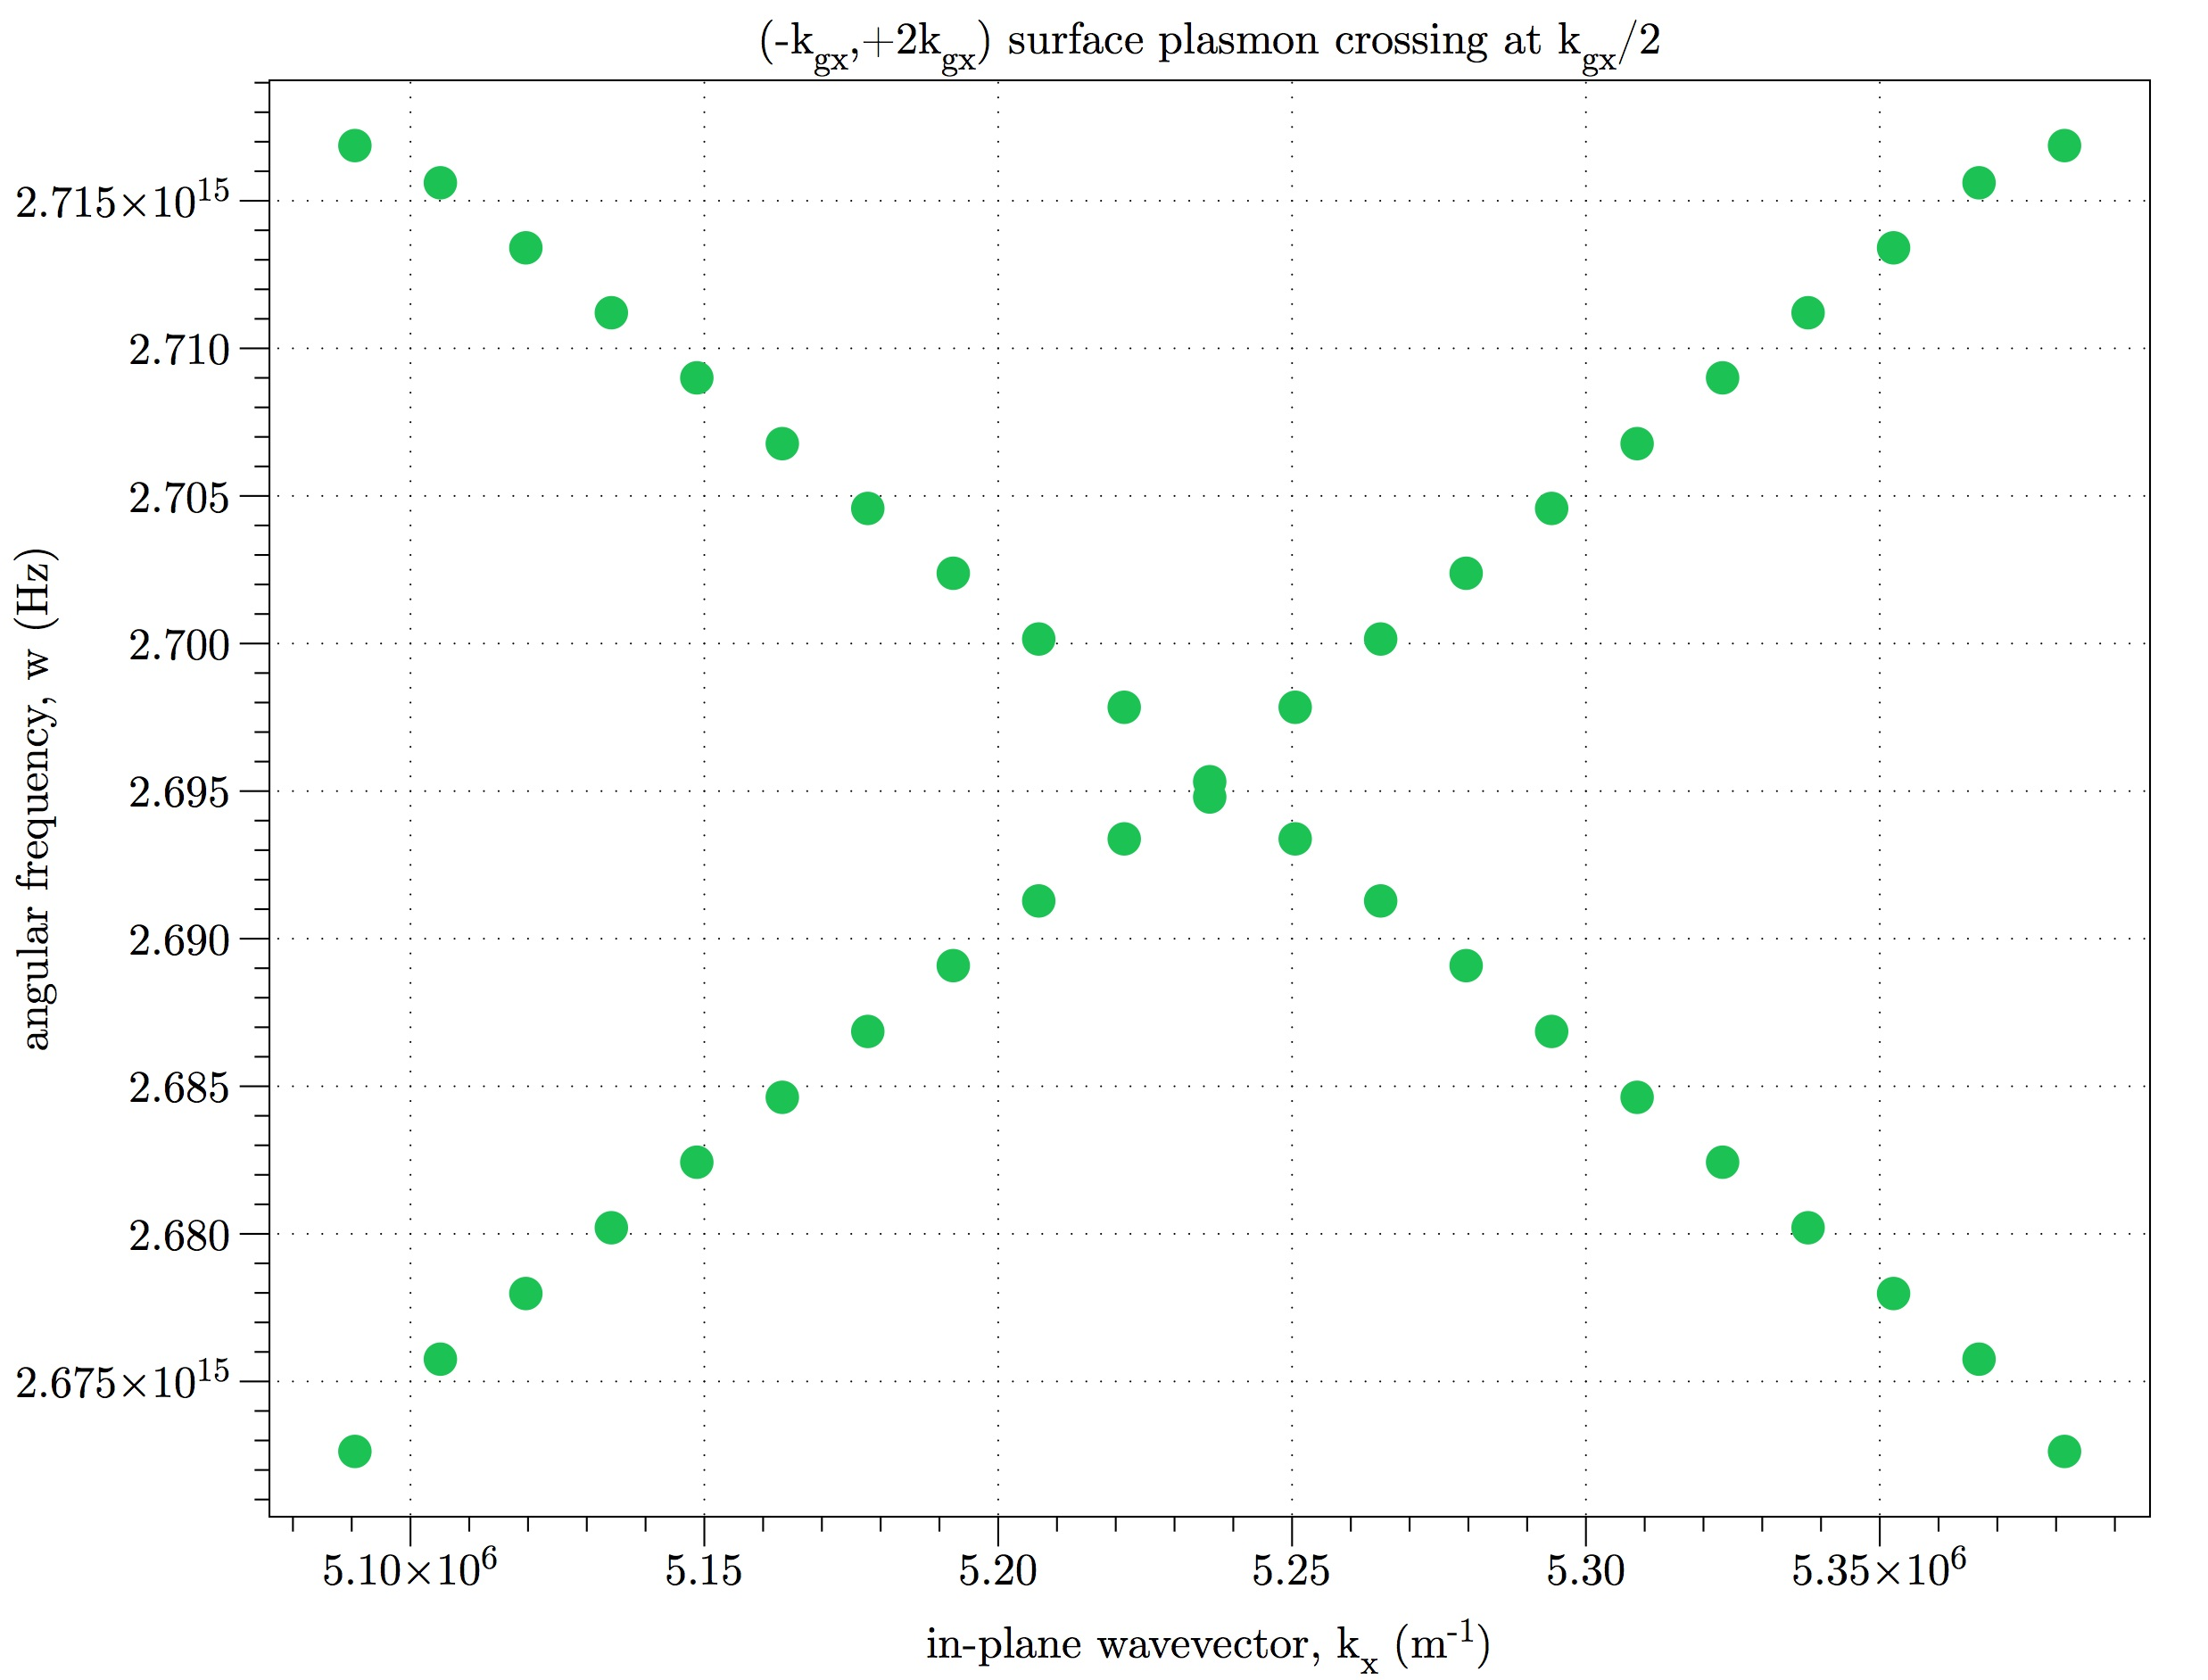
\includegraphics[width=\linewidth]{temp-bandgaps/2kgkg-150nm-yoffset.jpg}
\caption{}
\end{subfigure}
\begin{subfigure}[b]{0.3\linewidth}
\centering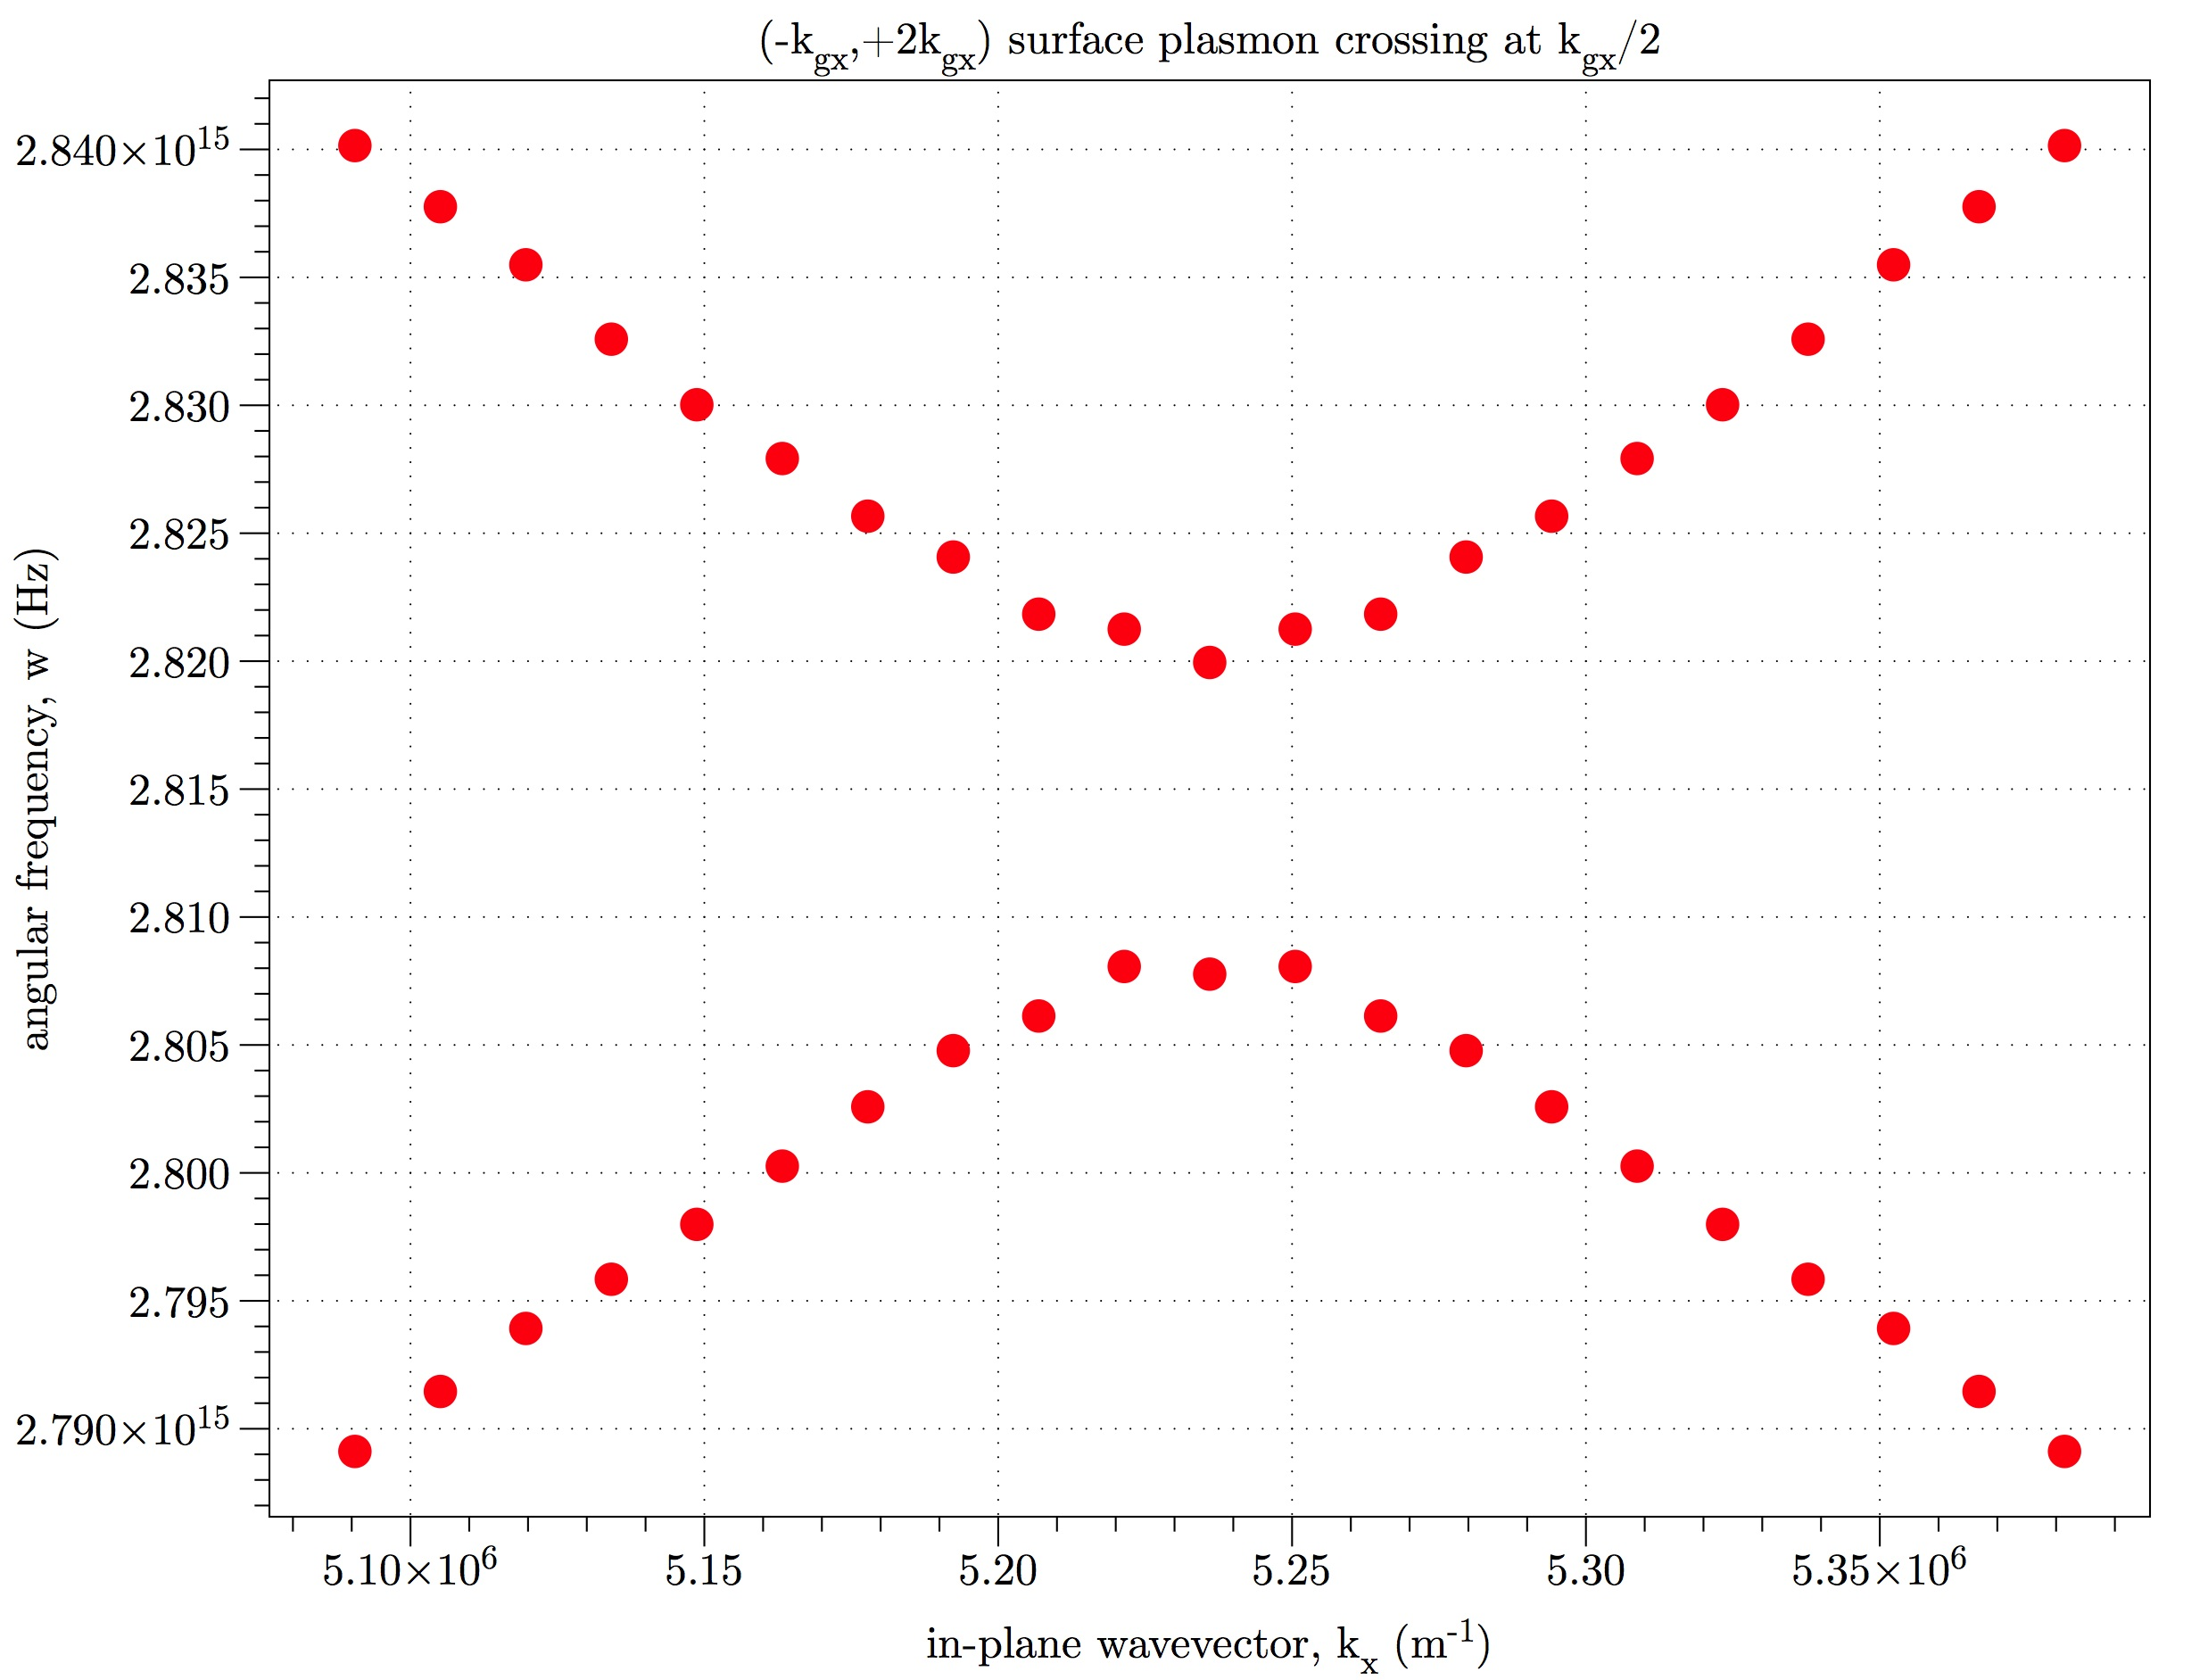
\includegraphics[width=\linewidth]{temp-bandgaps/2kg-kg-150nm-offset.jpg}
\caption{}
\end{subfigure}
\caption{Asymmetrizing the zig-zag causes bandgaos to open}
\end{figure}

With additional Fourier components present, direct scattering of SPP modes by values of $2k_g$ or greater are now possible, causing the SPP modes at normal incidence to couple strongly and form a larger bandgap than they might have using weak $k_g$-$k_g$ scattering. This is demonstrated in figure \ref:{?} which shows the equi-energy contours for SPPs on a symmetric and asymmetric zig-zag grating. It is clear that, at normal incidence, band gaps now form in the asymmetric case.

It is possible that the discussion about equivilent standing waves and 'no 2kg components' are the same discussion from different perspectives.
\section{Conclusions}
We have demonstrated experimentally and with FEM modeling the coupling of plane polarized light to SPPs on a metallic zig-zag grating. We have found that when the plane of incidence contains the zig-zag grating vector, odd-order diffracted SPPs couple only to TE polarized light and coupling to TM light is forbidden. At the first BZ boundary in this orientation, photonic band-gaps do not form because the two possible standing wave solutions along the zig-zag surface are equivalent in energy. Changing the zig-zag symmetry will allow control of the polarization selectivity of SPP coupling on such gratings, with asymmetric zig-zag gratings providing a route to polarization independent excitation of SPPs which propagate in the plane of diffraction.

\end{document}
